% This is the Reed College LaTeX thesis template. Most of the work
% for the document class was done by Sam Noble (SN), as well as this
% template. Later comments etc. by Ben Salzberg (BTS). Additional
% restructuring and APA support by Jess Youngberg (JY).
% Your comments and suggestions are more than welcome; please email
% them to cus@reed.edu
%
% See http://web.reed.edu/cis/help/latex.html for help. There are a
% great bunch of help pages there, with notes on
% getting started, bibtex, etc. Go there and read it if you're not
% already familiar with LaTeX.
%
% Any line that starts with a percent symbol is a comment.
% They won't show up in the document, and are useful for notes
% to yourself and explaining commands.
% Commenting also removes a line from the document;
% very handy for troubleshooting problems. -BTS

% As far as I know, this follows the requirements laid out in
% the 2002-2003 Senior Handbook. Ask a librarian to check the
% document before binding. -SN

%%
%% Preamble
%%
% \documentclass{<something>} must begin each LaTeX document
\documentclass[12pt,twoside]{reedthesis}
% Packages are extensions to the basic LaTeX functions. Whatever you
% want to typeset, there is probably a package out there for it.
% Chemistry (chemtex), screenplays, you name it.
% Check out CTAN to see: http://www.ctan.org/
%%
\usepackage{graphicx,latexsym}
\usepackage{amsmath}
\usepackage{amssymb,amsthm}
\usepackage{longtable,booktabs,setspace}
\usepackage{chemarr} %% Useful for one reaction arrow, useless if you're not a chem major
\usepackage[hyphens]{url}
% Added by CII
\usepackage{hyperref}
\usepackage{lmodern}
\usepackage{float}
\floatplacement{figure}{H}
% End of CII addition
\usepackage{rotating}

% Next line commented out by CII
%%% \usepackage{natbib}
% Comment out the natbib line above and uncomment the following two lines to use the new
% biblatex-chicago style, for Chicago A. Also make some changes at the end where the
% bibliography is included.
%\usepackage{biblatex-chicago}
%\bibliography{thesis}


% Added by CII (Thanks, Hadley!)
% Use ref for internal links
\renewcommand{\hyperref}[2][???]{\autoref{#1}}
\def\chapterautorefname{Chapter}
\def\sectionautorefname{Section}
\def\subsectionautorefname{Subsection}
% End of CII addition

% Added by CII
\usepackage{caption}
\captionsetup{width=5in}
% End of CII addition

% \usepackage{times} % other fonts are available like times, bookman, charter, palatino

% Syntax highlighting #22
  \usepackage{color}
  \usepackage{fancyvrb}
  \newcommand{\VerbBar}{|}
  \newcommand{\VERB}{\Verb[commandchars=\\\{\}]}
  \DefineVerbatimEnvironment{Highlighting}{Verbatim}{commandchars=\\\{\}}
  % Add ',fontsize=\small' for more characters per line
  \usepackage{framed}
  \definecolor{shadecolor}{RGB}{248,248,248}
  \newenvironment{Shaded}{\begin{snugshade}}{\end{snugshade}}
  \newcommand{\KeywordTok}[1]{\textcolor[rgb]{0.13,0.29,0.53}{\textbf{#1}}}
  \newcommand{\DataTypeTok}[1]{\textcolor[rgb]{0.13,0.29,0.53}{#1}}
  \newcommand{\DecValTok}[1]{\textcolor[rgb]{0.00,0.00,0.81}{#1}}
  \newcommand{\BaseNTok}[1]{\textcolor[rgb]{0.00,0.00,0.81}{#1}}
  \newcommand{\FloatTok}[1]{\textcolor[rgb]{0.00,0.00,0.81}{#1}}
  \newcommand{\ConstantTok}[1]{\textcolor[rgb]{0.00,0.00,0.00}{#1}}
  \newcommand{\CharTok}[1]{\textcolor[rgb]{0.31,0.60,0.02}{#1}}
  \newcommand{\SpecialCharTok}[1]{\textcolor[rgb]{0.00,0.00,0.00}{#1}}
  \newcommand{\StringTok}[1]{\textcolor[rgb]{0.31,0.60,0.02}{#1}}
  \newcommand{\VerbatimStringTok}[1]{\textcolor[rgb]{0.31,0.60,0.02}{#1}}
  \newcommand{\SpecialStringTok}[1]{\textcolor[rgb]{0.31,0.60,0.02}{#1}}
  \newcommand{\ImportTok}[1]{#1}
  \newcommand{\CommentTok}[1]{\textcolor[rgb]{0.56,0.35,0.01}{\textit{#1}}}
  \newcommand{\DocumentationTok}[1]{\textcolor[rgb]{0.56,0.35,0.01}{\textbf{\textit{#1}}}}
  \newcommand{\AnnotationTok}[1]{\textcolor[rgb]{0.56,0.35,0.01}{\textbf{\textit{#1}}}}
  \newcommand{\CommentVarTok}[1]{\textcolor[rgb]{0.56,0.35,0.01}{\textbf{\textit{#1}}}}
  \newcommand{\OtherTok}[1]{\textcolor[rgb]{0.56,0.35,0.01}{#1}}
  \newcommand{\FunctionTok}[1]{\textcolor[rgb]{0.00,0.00,0.00}{#1}}
  \newcommand{\VariableTok}[1]{\textcolor[rgb]{0.00,0.00,0.00}{#1}}
  \newcommand{\ControlFlowTok}[1]{\textcolor[rgb]{0.13,0.29,0.53}{\textbf{#1}}}
  \newcommand{\OperatorTok}[1]{\textcolor[rgb]{0.81,0.36,0.00}{\textbf{#1}}}
  \newcommand{\BuiltInTok}[1]{#1}
  \newcommand{\ExtensionTok}[1]{#1}
  \newcommand{\PreprocessorTok}[1]{\textcolor[rgb]{0.56,0.35,0.01}{\textit{#1}}}
  \newcommand{\AttributeTok}[1]{\textcolor[rgb]{0.77,0.63,0.00}{#1}}
  \newcommand{\RegionMarkerTok}[1]{#1}
  \newcommand{\InformationTok}[1]{\textcolor[rgb]{0.56,0.35,0.01}{\textbf{\textit{#1}}}}
  \newcommand{\WarningTok}[1]{\textcolor[rgb]{0.56,0.35,0.01}{\textbf{\textit{#1}}}}
  \newcommand{\AlertTok}[1]{\textcolor[rgb]{0.94,0.16,0.16}{#1}}
  \newcommand{\ErrorTok}[1]{\textcolor[rgb]{0.64,0.00,0.00}{\textbf{#1}}}
  \newcommand{\NormalTok}[1]{#1}

% To pass between YAML and LaTeX the dollar signs are added by CII
\title{Modeling Racially Disproportionate Language on Twitter during NFL Game
Play}
\author{Julianna Alvord}
% The month and year that you submit your FINAL draft TO THE LIBRARY (May or December)
\date{May 13, 2019}
\division{Statistical \& Data Sciences}
\advisor{Ben Baumer}
\institution{Smith College}
\degree{Bachelor of Arts}
%If you have two advisors for some reason, you can use the following
% Uncommented out by CII
\altadvisor{Randi Garcia}
% End of CII addition

%%% Remember to use the correct department!
\department{Statistical \& Data Sciences}
% if you're writing a thesis in an interdisciplinary major,
% uncomment the line below and change the text as appropriate.
% check the Senior Handbook if unsure.
%\thedivisionof{The Established Interdisciplinary Committee for}
% if you want the approval page to say "Approved for the Committee",
% uncomment the next line
%\approvedforthe{Committee}

% Added by CII
%%% Copied from knitr
%% maxwidth is the original width if it's less than linewidth
%% otherwise use linewidth (to make sure the graphics do not exceed the margin)
\makeatletter
\def\maxwidth{ %
  \ifdim\Gin@nat@width>\linewidth
    \linewidth
  \else
    \Gin@nat@width
  \fi
}
\makeatother

\renewcommand{\contentsname}{Table of Contents}
% End of CII addition

\setlength{\parskip}{0pt}

% Added by CII
  %\setlength{\parskip}{\baselineskip}
  \usepackage[parfill]{parskip}

\providecommand{\tightlist}{%
  \setlength{\itemsep}{0pt}\setlength{\parskip}{0pt}}

\Acknowledgements{
I want to thank my advisors, Ben and Randi, for their unwavering support
and willingness to share their expertise. I would also like to thank my
family and friends for putting up with me during this process.
}

\Dedication{

}

\Preface{

}

\Abstract{
Following the actions of Colin Kapernick in August of 2016, incidents
involving racially charged language towards NFL players became
widespread across many forms of social media. Previous studies offer
qualitative evidence of racially disproportionate negative language and
blame in sports contexts. We believe that this phenomenon is measureable
on a larger scale. This thesis seeks to quantify previous research by
first accessing the Twitter API then running a sentiment analysis to
determine the percentage of negative words for a subset of 24 NFL
players at 5 time points. We fit a multilevel regression model to test
our hypothesis that during a game that was lost, sentiments will be more
negative toward black players, whereas this difference will be smaller,
or zero, in games that were won. Additional variables including yards
and position were added to our model. Our results demonstrate that on
average, the percentage of negative words during a loss decreases by
7.22 percentage points for white players relative to black players,
holding position and yards constant. During a win, there is almost no
difference in the observed sentiment between white and black players.
}

	\usepackage{setspace}\doublespacing
	\usepackage{array}
% End of CII addition
%%
%% End Preamble
%%
%
\begin{document}

% Everything below added by CII
  \maketitle

\frontmatter % this stuff will be roman-numbered
\pagestyle{empty} % this removes page numbers from the frontmatter
  \begin{acknowledgements}
    I want to thank my advisors, Ben and Randi, for their unwavering support
    and willingness to share their expertise. I would also like to thank my
    family and friends for putting up with me during this process.
  \end{acknowledgements}

  \hypersetup{linkcolor=black}
  \setcounter{tocdepth}{2}
  \tableofcontents

  \listoftables

  \listoffigures
  \begin{abstract}
    Following the actions of Colin Kapernick in August of 2016, incidents
    involving racially charged language towards NFL players became
    widespread across many forms of social media. Previous studies offer
    qualitative evidence of racially disproportionate negative language and
    blame in sports contexts. We believe that this phenomenon is measureable
    on a larger scale. This thesis seeks to quantify previous research by
    first accessing the Twitter API then running a sentiment analysis to
    determine the percentage of negative words for a subset of 24 NFL
    players at 5 time points. We fit a multilevel regression model to test
    our hypothesis that during a game that was lost, sentiments will be more
    negative toward black players, whereas this difference will be smaller,
    or zero, in games that were won. Additional variables including yards
    and position were added to our model. Our results demonstrate that on
    average, the percentage of negative words during a loss decreases by
    7.22 percentage points for white players relative to black players,
    holding position and yards constant. During a win, there is almost no
    difference in the observed sentiment between white and black players.
  \end{abstract}

\mainmatter % here the regular arabic numbering starts
\pagestyle{fancyplain} % turns page numbering back on

\chapter{Introduction}\label{intro}

In August of 2016, San Francisco 49ers quarterback Colin Kaepernick
remained sitting by the team's water coolers during the National Anthem
prior to a preseason game. Immediately, the gesture was widely
questioned and criticized. Many fans found his actions to be
disrespectful to the sacrifices made by military members. After the
game, when asked by the NFL media why he refused to stand, Kaepernick
responded by stating, ``I am not going to stand up to show pride in a
flag for a country that oppresses black people and people of color''
(Hauser, 2016). His decision, along with his eventual exit from the NFL,
brought attention to racial injustice, peaceful protest, and their
connection to sports.

This event, while drawing criticism, also sparked conversations where
the main negative emotions ranged from disappointment to hatred. The
hateful language that flooded social media did not go unnoticed, and the
quarterback's image was tarnished beyond repair. Other black athletes,
especially those who support Kaepernick, paid a similar price. This
event created a connection between football and racially charged
language. Although Kaepernick is no longer an active player in the NFL,
his legacy, and the anger he fueled, is still evident. The analyses by
the media focused mainly on the negative language aimed both at
Kaepernick and other black players. However, most of these accounts were
anecdotal, referencing a few, seemingly isolated events. The aftermath
and lack of data-driven research on the topics addressed during this
event are the motivation behind this work.

We believe that this negative language towards black players in the NFL
is widespread and measurable. Given the relatively new techniques to
analyze language and sentiment on a larger scale, research in this area
is increasingly accessible to data scientists. Our goal is to quantify
and model the accounts of racially disproportionate language on social
media using these techniques in order to offer insight into the
connection between racial inequality and sport.

We conduct this research through two studies, both of which use data
from Twitter. The first study focuses on Super Bowl LIII and provides an
exploratory data analysis for the second, more balanced study. Here,
tweets are gathered for a selected subset of quarterbacks and receivers,
half of whom are white and half of whom are black. Our three-level
multilevel model is fit to the data from this study.

\section{Background}\label{background}

\subsection{Research Question}\label{research-question}

The main research question is as follows: Are sentiments on Twitter more
negative towards black NFL players after controlling for game outcome,
position, and quality of play?

\subsection{Racism in Sport}\label{racism-in-sport}

Although Colin Kaepernick's actions resulted in widespread media
attention, many previous studies have addressed issues of racism and
racial inequality in football and sports. Most often, these topics are
studied through the context of sports media. Early research began in
1977, where Rainville \& McCormick (1977) analysed covert forms of
prejudice in television broadcasts of nationally televised football
games. They found that white players were more likely to receive praise
for ``good'' plays and less likely to receive negative feedback for
``bad'' plays when compared to their black counterparts. More recently,
Angelini, Billings, MacArthur, Bissell, \& Smith (2014) analysed
broadcasts from the 2012 London Summer Olympics to determine whether
they revealed significant divergences in dialogues for athletes of
different racial groups. During this time, white athletes were more
likely to be mentioned and there were significant differences in the
commentary for white, black, latino, asian, and middle eastern athletes.

The relationship between racism and sport does not simply lie within the
media. However, racism in other areas of sports is not easy to
determine. Hylton \& Lawrence (2016) argues that while it is important
to contront frontstage racism, such as that observed in the media and in
other, more explicit ways, researchers must be mindful of more subvert
forms of racism within sport. Research on subvert forms of racism, such
as that from fans, is few and far between. This may be due to lack of
access to data. Many studies surrounding racist dialogue among fans rely
on survey data. Research from Cleland \& Cashmore (2014) drew from 2,500
responses from soccer fans to an anonymous survey, which aimed to
examine the extent of racism within the sport. They found that half of
respondents either witness or experience racism in some form.

As seen from Kaepernick's exile and from these previous studies, racism
in the NFL, whether apparent or more subvert, is widespread. Although
individuals questioning the protest cite military disrespect as their
main concern, a study from Intravia, Piquero, \& Piquero (2018) found
that on average, black respondents were more likely to support all types
of anthem protests and believe players who choose to participate should
not be punished, compared to white respondents. Those strong race
effects remain even after controlling for several key correlates,
suggesting that race is a key distinction between support and
disapproval of these NFL anthem protests.

Research on racism, both in sport and across other areas of society, is
vital to the well being of people and athletes of color. Numerous
studies investigate the relationships between racism and mental and
physical health. Williams (1999) found that stress due to stigma, along
with individual and institutional discrimination can adversely affect
health. Additionally, the study addressed how racism in the United
States is ``responsible for the development of an organized system of
policies and practices designed to create racial inequality.'' Due to
the powerful structure of this system, people of color are often forced
to hide their experiences. This prejudicial system leads to negative
outcomes for people of color, and this is no different in the context of
sports. In a study by Burdsey (2011), researchers found that all
athletes, both racial minorities and racial majorities, tend to downplay
the repercussions of racial microaggressions. Research using large-scale
data focusing on racist and racially disproportionate language is
necessary to bring attention to issues of racism in sport context and
the subsequent extensive negative consequences.

\subsection{Sentiment Analysis}\label{sentiment-analysis}

Research dating back to 2003 has illustrated the use of sentiment
analysis to identify how sentiments are expressed and whether the
expressions in a determined body of text indicate positive or negative
opinions towards the subject (Nasukawa \& Yi, 2003). Sentiments are
determined by processing the language and context of a text, usually by
a human being. Sentiment analysis works in a similar way, but also allow
for a more automated process of long or multiple texts.

Two types of methods for sentiment analysis are often employed and
discussed in the literature: machine-learning-based and lexical-based.
Machine-learning approaches mainly rely on supervised classification
methods, where labeled training data is required. This method can be
easily specified to fit one's data. However, there are issues of
over-fitting to training data which leads to low applicability to
testing data. Lexical-based methods use a predetermined list of words,
known as a lexicon, where each word is matched to one or more
sentiments. In order to achieve a similar level of specification as the
machine-learning-based methods, these lexicons must be thorough and
contextual to the project at hand (Gonçalves, Araújo, Benevenuto, \&
Cha, 2013).

Sentiment analysis is not a simple approach. The decision to use this
method in a project requires an understanding of the levels of
granularity that can be specified. Early research tended to analyze
sentiments of entire documents, which can lower the accuracy of the
overall polarity assessment (Zhang, Zeng, Li, Wang, \& Zuo, 2009).
Instead, Meena \& Prabhakar (2007) employ sentence-level analyses in
order to focus on pieces, such as conjunctions, which can significantly
change overall sentiment.

For projects such as this one, whose main purpose is to employ sentiment
analysis to research a given topic instead of researching sentiment
analysis itself, there will be issues of accuracy. The reason for this
is that basic sentiment analyses focus on words individually to
determine overall sentiment; conjunctions will not be addressed.
Consider the phrase ``not good''. Using the method introduced below, the
phrase would be separated into ``not'' and ``good'', where ``good''
would be categorized as positive and ``not'' would be ignored
altogether. More details on how cases such as this are handled in this
study can be found below.

A simple process for conducting basic natural language processing and
sentiment analyses in R is detailed by Silge \& Robinson (2018). Here,
the authors use the tidy text format, which is described as
one-token-per-row. Therefore, each word is a row which allows for an
easy join to a lexicon that is specified to the project.

\subsection{Sentiment Analyses of Twitter and other Online
Data}\label{sentiment-analyses-of-twitter-and-other-online-data}

The goal of this project is to measure sentiments of football fans by
obtaining social media data. Thus, it is necessary to determine which
site would offer the proper information. We found that Twitter data is
commonly used for large-scale sentiment analyses as it is a ``massive
social networking site'' aimed at quick communication. Approximately 400
million tweets are published daily from Twitter's 140 million active
users (Kumar, Morstatter, \& Liu, 2014). Due to its constant stream of
data, many researchers utilize Twitter data for sentiment analysis
projects.

Our expectation that negative sentiments will be widespread throughout
Twitter is backed by much research. Awan (2014) examined 500 tweets to
determine how Muslim individuals are being viewed and targeted by
Twitter users. They found that ``the Internet and social media sites
such as Twitter have become a popular arena for online hate, partly due
to their accessibility and the anonymity they offer for offenders who
use it to intimidate, harass, and bully others.''

Anonymity plays a huge role in online hate and abuse found on Twitter.
Christopherson (2007) discussed the positive and negative results of
online anonymity. On the positive side, they offered privacy as an
example. Online users can decide how much of themselves to share with
others, which can have a positive effect on psychological well-being. On
the negative side, the authors connect the theory of group polarization
to online anonymity. They define group polarization as the ``tendency
for like-minded individuals to become more extreme in their thinking
following a group discussion.'' To connect back to the current project,
our hypothesis is supported by our belief that many football fans are
like-minded and Twitter offers an anonymous platform for anti-black
sentiments to become more extreme.

The anonymity of the Internet allows for hate speech and anti-black
sentiments to thrive for another reason. Racist comments can be made on
social media sites more freely and without consequence compared with
offline face-to-face interactions. Online anonymity provides individuals
with a sense of identity disguise or social distance from others which
in turn leads to the disclosure of racist ideologies with minimal
oversight (Keum \& Miller, 2018).

Cleland (2014) found specific evidence of racism online in a sports
context. Their study examined 500 posts from an online message board to
determine the level and nature of racist language among European
Football fans. They found extensive racist and Islamaphobic examples
throughout the platform, many of which took place during fan
interaction. These online incidents followed two high-profile incidents
of racism on the field in 2011 in the UK. Some black players responded
by reporting racist messages to the proper authorities while others were
forced to remain silent. This matches King (2004) argument that black
players often succeed \emph{despite} racism. He describes that many
black players are required to ``play the white man'' in order to be
accepted.

Focusing on Twitter, Stephens (2013) tracked over 150,000 accounts of
public racist tweets over the course of the year. This suggests that
racist language is present on Twitter. Also, sports fan involvement has
increased in the past few years with the introduction of game-specific
hashtags that guide conversation (Weller, Bruns, Burgess, Mahrt, \&
Puschmann, 2014). Expanded Twitter activity prompts fan interactions and
further data of game reactions, making tweets the ideal text for this
project.

\subsection{Multi-Level Modeling}\label{multi-level-modeling}

This project uses data that is grouped at different levels, where the
processes occurring at a higher level influence the processes of a lower
level. The levels in this case include team, individual players, and
time. Specifically, time points are nested within the player level and
players are nested within teams. Data that is structured in a
heirarchical way is often found within social science contexts, due
especially to natural groupings that occur with humans. Longitudinal
data, such as the data in this study, also creates heirarchical
structure as multiple data points for one individual are present. In
order to test the hypothesis and answer the research question for this
project, multilevel models are necessary. If we chose to use simpler
modeling techniques in this situation, serious theoretical and
statistical issues would be present. Those methods are employed with the
assumption that the data is independent. However, given that
longitudinal (and otherwise heirarcical) data includes multiple
observations for one individual, that assumption is violated.

Two fallacies that can occur when applying non-multilevel modeling
techniques on leveled data are ecological fallacies and atomistic
fallacies. The first occurs when patterns observed for groups are
assumed to hold true for individuals when this is not necessarily true.
The latter occurs when the opposite occurs, namely that patterns
observed for individuals are assumed to hold true for groups (Luke,
2004).

\section{Our Contribution}\label{our-contribution}

\subsection{Our Results}\label{our-results}

On average, the percentage of negative words during a loss decreases by
7.22\% for white players relative to black players, holding position and
yards constant. During a win, there is almost no observed difference in
sentiment between white and black players. This provides some evidence
for racial bias of football fans on Twitter.

\subsection{Reproducible Research}\label{reproducible-research}

As statistical analyses of data become increasingly common and complex,
reproducibility becomes increasingly necessary. In order for research to
be reproducible, proper documentation of methodology is crucial.
However, this is not practiced by many researchers, especially due to
the lack of proper technology. One way to improve statistical
reproducibility, a term used by Stodden (2014), is by utilizing
RMarkdown, an open source markup language. This tool allows for better
workflow, by combining a statistical package with a layout package
(Baumer, Cetinkaya-Rundel, Bray, Loi, \& Horton, 2014).

Given both the importance of reproducibility and the social relevance of
this project, we use R Markdown throughout a majority of the cleaning
and analyzing processes. However, gathering the data for one aspect this
project required the use of Python. For this process, we use Jupyter
Notebook, an open-source web application.

This thesis is being written using the \texttt{thesisdown} package in
\texttt{R} (Solomon, 2019). \texttt{Thesisdown} was inspired by the
\texttt{bookdown} package and offers an R Markdown template for
undergraduate theses (Xie, 2016).

All of the documents from this project, whether they be R Markdown
documents or Jupyter Notebooks, have been committed to
\href{https://github.com/jalvord1/nfl_sentiment}{GitHub}, a code hosting
platform (\emph{Hello world}, 2019). Github allows for easy code sharing
and collaboration between researchers, making it the ideal platform to
aid with reproducibility.

\chapter{Ethics}\label{ethics}

\section{Data Ethics Overview}\label{data-ethics-overview}

The recent increases in data access offer a unique opportunity for
companies and researchers to make insights that would otherwise be
impossible. These insights could lead to better disease tracking,
optimization of business practices, or streamlining of the hiring
process, to name a few examples. The benefits of using data in research
across all disciplines are extensive and cannot be understated. However,
ensuring that the data usage is ethical and fair is a vital step in the
process.

As helpful as data can be, it can be equally as damaging and dangerous
if used without consideration of the ethical consequences. Mittelstadt
\& Floridi (2016) state that researchers using big data must have
ethical foresight instead of ethical hindsight, as the consequences of
unethical data use are substantial. Despite the importance of data
ethics, many people do not focus on ethics or issues of bias. Often,
these issues stem from a lack of contextual understanding of data and
data science techniques (Taylor, 2016). Additionally, there is a lack of
a universal code of conduct for data scientists. One that is currently
available comes from National Academies of Sciences, Medicine, \& others
(2018). Although data can be used by researchers in any domain,
knowledge of ethical issues of statistics and data analysis is not
widespread. We will begin by combining multiple sources to create a
thorough ethics guide for this project, specifically relating to
research involving web scraping.

\subsection{Theory-Driven Web
Scraping}\label{theory-driven-web-scraping}

Landers, Brusso, Cavanaugh, \& Collmus (2016) argue that when scraping
data from the web, researchers must follow a hypothetico-deductive
modeling approach. This means that data is scraped with a hypothesis in
mind and is gathered in order to test the hypothesis or answer a
research question. This directs researchers away from hypothesizing
after the results are already known. When data is scraped without a
specific research question and the study design is unbalanced, it may be
more likely for issues of content or construct validity to occur. These
may go undetected and demonstrate results that do not accurately
represent the phenomenon. The concept of creating a hypothesis after
data is collected and analyzed is known as \emph{post-hoc
hypothesizing}. It is important to differentiate between presenting
post-hoc hypotheses as a priori (PPHA) and presenting post-hoc
hypotheses as those which require future empirical verification (Leung,
2011). The latter represents an acceptable process of research, whereas
the former is considered unethical in most research domains.

Leung (2011) specifies three types of widespread PPHA. In the first
case, researchers create hypotheses directly from their results in order
for their study to be theoretically compelling. In the second case,
researchers will simply drop hypotheses that are dis-confirmed and fail
to introduce them at all. In the third and final case, hypotheses may be
added that appear to match the results but are presented as a priori.
These methods lack the transparency necessary for ethical research
practices. This type of post-hoc hypothesizing fails to account for
previously studied relevant theoretical concepts, an important aspect of
the research process. These issues can be magnified when using data
scraped from the web, as larger sample sizes could lead to more
statistically significant results. These studies may be more likely to
be accepted for publication and therefore, ethically questionable
research may direct future work on the topic.

Additionally, investigators must recognize that results using scraped
data cannot be generalized to the entire population, even if the sample
appears widespread. The reason for this, specified by Wallace (2015), is
that Internet users are inherently different than those who are not on
the Internet. If the goal is to generalize toward other Internet users,
that is acceptable in certain cases. However, it is unethical to assume
results can be generalized any further.

\subsection{Identifiability}\label{identifiability}

Another important ethical issue of web scraping that must be considered
is identifiability. Data from online sources often contain identifying
information, even if it does not initially appear so. Data that can be
used to distinguish or trace identities either alone or in combination
with other information that is linkable to an individual is known as
personally identifiable information (PII) (Krishnamurthy \& Wills,
2009). Given the huge increase in social network use, scandals involving
data from these sources have been all over the news. Facebook, in
particular, has come under scrutiny for their lack of data privacy and
transparency. In 2008, Facebook announced that an attack on their
servers resulted in the exposure of the personal data of over 50 million
users (Rosen, 2018). While alarming, PII can be leaked without security
breaches. The ability for researchers to use APIs or other computer
science techniques to scrape data from these sites has also resulted in
an unethical distribution of PII. As an example, researchers Emil
Kirkegaard and Julius Daugbjerg Bjerrekær scraped data from OkCupid, and
then released the data set for other researchers to use. However, the
data included identifiable information of users, including their sexual
preferences, politics, and feelings about homosexuality, among others
(Resnick, 2016).

When Kirkegaard was questioned about this ethical breach, he argued that
the data were already public and therefore their scraped data was simply
making the information accessible for research (Resnick, 2016). This
example brings light to the delicate balance of data accessibility and
privacy. While reproducibility of research is important, avoiding
ethical issues that arise with PII must be given equal attention. Often,
determining that line is left up to the discretion of the researcher.
Therefore, it is necessary for researchers to be constantly aware of the
ethical consequences of gathering and sharing data. In the context of
the OkCupid example and the argument from the primary investigator,
while the data was technically public, the users did not consent for
their data to be used and shared for research outside of the OkCupid
website.

Sharing PII can result in consequences that extend beyond simply a lack
of consent. Floridi \& Taddeo (2016) warn that it can lead to serious
problems that range from group discrimination (racism, sexism, ageism,
etc.) to group-targeted forms of violence. When evaluating the multiple
ethical concerns of big data research, one solution is to follow the two
moral duties introduced by Floridi (2014): to foster human rights and
improve human welfare. If that is the ultimate goal of the research,
ethical concerns will be minimized.

\subsection{Connection to this
Research}\label{connection-to-this-research}

Throughout the process of this research, we address and attempt to avoid
any and all ethical concerns. First, we follow the theory-driven web
scraping approach in the second study when connecting to the Twitter API
to gather tweets. Our study is designed purposefully to answer our
research question and test our hypothesis. We do not hypothesize
post-hoc a priori nor do we generalize our results to populations past
football fans who use Twitter. In the first study, we did not
necessarily follow a theory-driven web scraping approach but we also did
not fit models or perform any statistical inference tests.

While gathering tweets through the Twitter streaming and full-archive
APIs, we only select certain meta-data to be included in our final data
sets. These do not include usernames, IDs, or other personally
identifiable information. Our goal is to analyze sentiments from the
words of the tweets and this process is not at all related to the
specific users who produced said tweets. As the code we use to gather
the tweets is uploaded to GitHub, another researcher could alter the
functions we wrote to include identifying variables into the data set.
That being said, the only identifiable data that could be gathered is a
person's handle. This cannot be used to link to other demographic data.

\chapter{Study 1- Super Bowl LIII Exploratory Data
Analysis}\label{study-1--super-bowl-liii-exploratory-data-analysis}

\section{Introduction}\label{introduction}

The goal of this initial study is to explore tweet data aimed at
football players. As will be explained further in the next chapter,
there are significant limits on gathering Twitter data that is part of
their full archive (tweets that were published prior to seven days
earlier). Therefore, we decided it is important to gather additional
data that is not limited in order to perform preliminary analyses.

Twitter offers many methods for accessing its data. A few examples
include a premium search of the full archive, a standard search, and a
filter of real-time tweets. Each of these has specific limits, some more
stringent than others. However, the method that allows for the largest
amount of tweets is the real-time filtering method. Here, a query and
time period are specified and a subset of tweets that match the query
are gathered for the length of the time period.

We use Super Bowl LIII for this aspect of the project. We believe that
this event would offer an abundance of data, given the amount of data
amassed during previous Super Bowls. Last year, over 100 million people
watched the Super Bowl (Statista, 2019) and in 2017, 27.6 million tweets
were posted relating to the Super Bowl (Sarah Perez, 2017).

We did not begin this project with any specific hypotheses or research
questions as it is more exploratory in nature. Our main goals are to
determine what the most tweeted words were, how many tweets were posted
per player, and what the average sentiments were per player. Unlike in
the next study, we are not modeling the data.

\section{Methods}\label{methods}

\subsection{Creating a Query}\label{creating-a-query}

The first step of this study is to determine what our query would be.
The standard option for filtering real-time tweets allows for up to 400
keywords and 5,000 user ids (\emph{Filtering realtime Tweets}, 2019). As
our focus was on players, we are using the roster of the starting
players for each team as the query. The roster is pulled from the CBS
Sports website, the network that hosted the game. Their full names were
added to a column in a \texttt{csv} file. Each team had 25 starting
players, for a total of 50 altogether. Next, in order to increase the
data that would be gathered, we added each player's Twitter handle to
the next column. The gathering of player names and Twitter handles is
done by hand, and manually entered into the file.

In addition to the names and twitter handles, the race of the players is
added to the data file, which was based entirely on our perceptions. We
used the official NFL roster photo of each player to record their race
based on what we believed it to be from that photo.

Once in R, we make the full name and Twitter handle columns into lists
and then combine the two. This list is saved as an object for use in the
function that gathers live tweets.

\subsection{Using the rtweet Function}\label{using-the-rtweet-function}

The \texttt{rtweet} package in R is designed to give access to Twitter's
Rest and Streaming APIs (Kearney, 2018). To begin using the functions of
this package, users must first become an authorized developer by Twitter
Inc., a process that can be done online. Once accepted as a developer,
one must create an ``app'', which in turn, will then create tokens
necessary to access the API through functions in the \texttt{rtweet}
package.

Once created, a simple function called \texttt{create\_token()} connects
to the app and saves your token to your environment. This means the
following code only needs to be run once.

\small
\begin{Shaded}
\begin{Highlighting}[]
\KeywordTok{create_token}\NormalTok{(}
  \DataTypeTok{app =} \StringTok{"my_twitter_research_app"}\NormalTok{,}
  \DataTypeTok{consumer_key =} \StringTok{"aaaaaaaa"}\NormalTok{,}
  \DataTypeTok{consumer_secret =} \StringTok{"bbbbbbbb"}\NormalTok{,}
  \DataTypeTok{access_token =} \StringTok{"cccccccc"}\NormalTok{,}
  \DataTypeTok{access_secret =} \StringTok{"dddddddd"}
\NormalTok{  )}
\end{Highlighting}
\end{Shaded}
\normalsize

The next step is to decide the length of time that the function would
run to collect tweets. Super Bowl LIII began at 6:30pm E.T. and was
expected to last approximately four hours. We ran the function for seven
hours beginning at 5:30. This would allow us to gather the tweets posted
leading up to the game as well as those posted immediately following the
game. We believe reaction tweets would be posted both during game play
and in the hours following. The following code is used to load the query
data, make a list that included full names and Twitter handles, and
gather the streaming tweets.

\small
\begin{Shaded}
\begin{Highlighting}[]
\CommentTok{#reading in the data}
\NormalTok{starters <-}\StringTok{ }\KeywordTok{read_csv}\NormalTok{(}\KeywordTok{here}\NormalTok{(}\StringTok{"sb analysis"}\NormalTok{, }\StringTok{"sb_starters.csv"}\NormalTok{))}

\CommentTok{#pulling out player names}
\NormalTok{name <-}\StringTok{ }\KeywordTok{pull}\NormalTok{(starters, players)}

\CommentTok{#cleaning twitter column, selecting that column, then }
\CommentTok{#filtering out those without twitter handle}
\NormalTok{twitter_clean <-}\StringTok{ }\NormalTok{starters }\OperatorTok
\StringTok{  }\KeywordTok{mutate}\NormalTok{(}\DataTypeTok{twitter_clean =} \KeywordTok{gsub}\NormalTok{(}\StringTok{"'"}\NormalTok{, }\StringTok{""}\NormalTok{, twitter)) }\OperatorTok
\StringTok{  }\KeywordTok{select}\NormalTok{(twitter_clean) }\OperatorTok
\StringTok{  }\KeywordTok{filter}\NormalTok{(}\OperatorTok{!}\NormalTok{twitter_clean }\OperatorTok{==}\StringTok{ ""}\NormalTok{)}

\CommentTok{#pulling out twitter handles}
\NormalTok{twitter <-}\StringTok{ }\KeywordTok{pull}\NormalTok{(twitter_clean, twitter_clean)}

\CommentTok{#full name and twitter handle for streaming}
\NormalTok{full <-}\StringTok{ }\KeywordTok{c}\NormalTok{(name, twitter)}

\CommentTok{# Stream keywords used to filter tweets}
\NormalTok{q <-}\StringTok{ }\KeywordTok{paste}\NormalTok{(full, }\DataTypeTok{collapse =} \StringTok{','}\NormalTok{)}

\CommentTok{# stream time is in seconds}
\CommentTok{# ( x * 60 * 60 = x hours)}
\CommentTok{# Stream for 7 hours}
\NormalTok{streamtime <-}\StringTok{ }\DecValTok{7} \OperatorTok{*}\StringTok{ }\DecValTok{60} \OperatorTok{*}\StringTok{ }\DecValTok{60}

\NormalTok{## Filename to save json data (backup)}
\NormalTok{filename <-}\StringTok{ }\KeywordTok{here}\NormalTok{(}\StringTok{"sb analysis"}\NormalTok{, }\StringTok{"sb_tweets.json"}\NormalTok{)}

\CommentTok{#save as json for later parsing}
\KeywordTok{stream_tweets}\NormalTok{(}\DataTypeTok{q =}\NormalTok{ q, }\DataTypeTok{timeout =}\NormalTok{ streamtime, }
              \DataTypeTok{file_name =}\NormalTok{ filename, }\DataTypeTok{parse =} \OtherTok{FALSE}\NormalTok{, }\DataTypeTok{language =} \StringTok{"en"}\NormalTok{)}
\end{Highlighting}
\end{Shaded}
\normalsize

As shown above, the list of twitter handles and names needs to be
formatted as a single string with a comma separating each value that
tweets would be matched against. Additionally, the stream time must be
in seconds so the numbers of hours chosen, in this case 7, needs to be
multiplied by 3,600. Finally, in our \texttt{stream\_tweets()} function,
we include the parameter \texttt{parse\ =\ FALSE} which saves the tweets
as a \texttt{json} file to disk instead of loading the file directly to
my environment. Later, we parsed this \texttt{json} file using an
additional function within the \texttt{rtweet} package.

\small
\begin{Shaded}
\begin{Highlighting}[]
\CommentTok{#parsing entire file}
\NormalTok{rt <-}\StringTok{ }\KeywordTok{parse_stream}\NormalTok{(filename)}
\end{Highlighting}
\end{Shaded}
\normalsize

\subsection{Cleaning}\label{cleaning}

Once the file is parsed, it is loaded into our environment for cleaning.
The file contained 618,628 rows and 88 variables. These 88 variables
each contain a piece of metadata that is provided by Twitter. Some
variables include \texttt{user\_id}, \texttt{created\_at}, and
\texttt{is\_retweet}. The next step is to clean the text in order to
pull out the names or twitter handles contained in the tweets in order
to determine which players the tweet is mentioning.
\begin{longtable}[]{@{}llll@{}}
\caption{\label{tab:sumstat} Summary statistics of the Super Bowl tweets
analysis}\tabularnewline
\toprule
\begin{minipage}[b]{0.20\columnwidth}\raggedright\strut
Number of Tweets\strut
\end{minipage} & \begin{minipage}[b]{0.22\columnwidth}\raggedright\strut
Number of variables\strut
\end{minipage} & \begin{minipage}[b]{0.20\columnwidth}\raggedright\strut
Number of players\strut
\end{minipage} & \begin{minipage}[b]{0.25\columnwidth}\raggedright\strut
Number of Twitter Handles\strut
\end{minipage}\tabularnewline
\midrule
\endfirsthead
\toprule
\begin{minipage}[b]{0.20\columnwidth}\raggedright\strut
Number of Tweets\strut
\end{minipage} & \begin{minipage}[b]{0.22\columnwidth}\raggedright\strut
Number of variables\strut
\end{minipage} & \begin{minipage}[b]{0.20\columnwidth}\raggedright\strut
Number of players\strut
\end{minipage} & \begin{minipage}[b]{0.25\columnwidth}\raggedright\strut
Number of Twitter Handles\strut
\end{minipage}\tabularnewline
\midrule
\endhead
\begin{minipage}[t]{0.20\columnwidth}\raggedright\strut
618628\strut
\end{minipage} & \begin{minipage}[t]{0.22\columnwidth}\raggedright\strut
88\strut
\end{minipage} & \begin{minipage}[t]{0.20\columnwidth}\raggedright\strut
50\strut
\end{minipage} & \begin{minipage}[t]{0.25\columnwidth}\raggedright\strut
42\strut
\end{minipage}\tabularnewline
\bottomrule
\end{longtable}
Two variables contain text that is useful for our analysis. One is
\texttt{text}, which contains the actual encoded string of the status
update. However, some tweets in the data were quoted, meaning users
added comments to an already published tweet. This text is found in the
variable \texttt{quoted\_text}. Using the \texttt{tolower()} function (R
Core Team, 2018), we translate the text from these two columns from a
mix of upper and lower case characters to only lower case. Then, using
the \texttt{paste()} function, we create another column that combines
the text from these two lower case character vectors. Once this column
is created, we determine if there are duplicate tweets by using the
\texttt{duplicated()} function.

\small
\begin{table}[!h]

\caption[Number of Duplicated Tweets]{\label{tab:unnamed-chunk-6}Number of Duplicated Tweets}
\centering
\begin{tabular}{l|r}
\hline
dup & n\\
\hline
FALSE & 220397\\
\hline
TRUE & 398231\\
\hline
\end{tabular}
\end{table}
\normalsize
In total, 398,231 tweets contained duplicate text. We believed that the
majority of those would have been retweeted tweets. Using the
\texttt{grepl()} function, we could determine if the text contained the
string \texttt{rt}, indicating that the tweet may be a retweeted text.
\begin{Shaded}
\begin{Highlighting}[]
\CommentTok{#how many of the dups have rt at all}
\NormalTok{full_duptab <-}\StringTok{ }\NormalTok{full }\OperatorTok
\StringTok{  }\KeywordTok{filter}\NormalTok{(dup }\OperatorTok{==}\StringTok{ }\OtherTok{TRUE}\NormalTok{) }\OperatorTok
\StringTok{  }\KeywordTok{mutate}\NormalTok{(}\DataTypeTok{rt =} \KeywordTok{grepl}\NormalTok{(}\StringTok{"rt"}\NormalTok{, full_text_low)) }\OperatorTok
\StringTok{  }\KeywordTok{group_by}\NormalTok{(rt) }\OperatorTok
\StringTok{  }\KeywordTok{summarise}\NormalTok{(}\DataTypeTok{n =} \KeywordTok{n}\NormalTok{()) }
\end{Highlighting}
\end{Shaded}
\begin{table}[!h]

\caption[Number of Duplicated Tweets with `rt` String]{\label{tab:rttweets}Number of Duplicated Tweets with `rt` String}
\centering
\begin{tabular}{l|r}
\hline
rt & n\\
\hline
FALSE & 312215\\
\hline
TRUE & 86016\\
\hline
\end{tabular}
\end{table}
In \ref{tab:rttweets}, Only 86,016 of the tweets contained this string.
We are leaving the duplicate indicator variable in the data frame but
did not make a decision about how to handle them at this stage. Instead,
we save this cleaned data frame as another \texttt{rda} file to be used
for simple natural language processing and sentiment analyses.

\subsection{Matching Tweets to
Players}\label{matching-tweets-to-players}

Now that we have a data set containing all tweets and a cleaned text
column, we want to determine which tweets mentioned which players in
order to properly analyze the data. We start by creating the same list
of names and twitter handles that is used as the query within our
\texttt{stream\_tweets()} function. However, this time, the list is made
into a single string with the vertical bar separating each element.
Then, we use the same \texttt{tolower()} function as above to change
each character to lower case, in order to properly match the cleaned
text variable.

\small
\begin{Shaded}
\begin{Highlighting}[]
\CommentTok{#making list for str_extract_all function}
\NormalTok{all_players <-}\StringTok{ }\KeywordTok{paste}\NormalTok{(full_name, }\DataTypeTok{collapse =} \StringTok{'|'}\NormalTok{)}

\CommentTok{#lower case names and twitter handles}
\NormalTok{all_players_low =}\StringTok{ }\KeywordTok{tolower}\NormalTok{(all_players)}
\end{Highlighting}
\end{Shaded}
\normalsize

We employ the function \texttt{str\_extract\_all()} from the
\texttt{stringr} package (Wickham, 2019) to test whether the text column
contains any of the name or Twitter handles. A list-column is created
because many of the tweets match multiple names or twitter handles (when
multiple players are mentioned in one tweet). Then, to create a data
frame which duplicates the tweet for each player mentioned, we use the
\texttt{unnest()} function from the \texttt{tidyr} package (Wickham \&
Henry, 2018). This function takes a list-column then makes each element
of the list its own row. We show examples in Table
\ref{tab:unnesttweets}.

\small
\begin{Shaded}
\begin{Highlighting}[]
\NormalTok{full_more <-}\StringTok{ }\NormalTok{full }\OperatorTok
\StringTok{ }\CommentTok{#pulling out the players from either text or quoted text}
\StringTok{ }\KeywordTok{mutate}\NormalTok{(}\DataTypeTok{name_text =} \KeywordTok{str_extract_all}\NormalTok{(full_text_low, }
                                    \DataTypeTok{pattern =}\NormalTok{ all_players_low))}

\CommentTok{#unnesting the name_text list column}
\NormalTok{full_more_unnest <-}\StringTok{ }\NormalTok{full_more }\OperatorTok
\StringTok{  }\KeywordTok{unnest}\NormalTok{(name_text) }
\end{Highlighting}
\end{Shaded}
\normalsize
\begin{table}[!h]

\caption[Examples of Unnested Tweet Data Frame]{\label{tab:unnesttweets}Examples of Unnested Tweet Data Frame}
\centering
\begin{tabular}{>{\raggedright\arraybackslash}p{4.2cm}|>{\raggedright\arraybackslash}p{4.2cm}|>{\raggedright\arraybackslash}p{4.2cm}}
\hline
full\_text\_low & dup & name\_text\\
\hline
stephen gostkowski misses the 46-yard fg! https://t.co/jeuct0obcr,NA & TRUE & stephen gostkowski\\
\hline
not buying this one bit.. https://t.co/1trff1xyux,sean mcvay: todd gurley's performance simply a lack of opportunity https://t.co/qd1efgfudj & FALSE & todd gurley\\
\hline
are we gonna act like tom brady and robert kraft didn’t just kiss? https://t.co/qq5xlgpwsq,NA & TRUE & tom brady\\
\hline
rams tackle andrew whitworth on the super bowl: "at the end of the day we're all gonna die",NA & TRUE & andrew whitworth\\
\hline
in depth breakdown: tom brady super bowl 53 https://t.co/88dg2btbvy,NA & TRUE & tom brady\\
\hline
\end{tabular}
\end{table}
Once complete, it is necessary to filter the data set to include only
tweets that mentioned a player by their handle. To do so, we use the
\texttt{grepl()} function to determine if the new column that pulled out
the name or handles from the tweet begins with the \texttt{@} sign.
Then, the other tweets are saved into a different data frame. Each was
subsequently joined with the initial starter data set. Finally, we
combine these two data sets and two new columns are created. One fills
in the twitter handles for the tweets that mention a name and the other
fills in the names for the tweets that mention a handle.

\small
\begin{Shaded}
\begin{Highlighting}[]
\CommentTok{#lowering twitter handles and player names for join}
\NormalTok{starters_clean <-}\StringTok{ }\NormalTok{starters }\OperatorTok
\StringTok{  }\KeywordTok{mutate}\NormalTok{(}\DataTypeTok{twitter_clean =} \KeywordTok{sub}\NormalTok{(}\StringTok{"'"}\NormalTok{, }\StringTok{""}\NormalTok{, twitter),}
         \DataTypeTok{twitter_clean2 =} \KeywordTok{tolower}\NormalTok{(twitter_clean),}
         \DataTypeTok{name_clean =} \KeywordTok{tolower}\NormalTok{(players)) }\OperatorTok
\StringTok{  }\KeywordTok{select}\NormalTok{(}\OperatorTok{-}\KeywordTok{c}\NormalTok{(players, twitter, twitter_clean))}

\CommentTok{#filtering for tweets that mention a player by their @}
\NormalTok{tweets_names <-}\StringTok{ }\NormalTok{full_more_unnest }\OperatorTok
\StringTok{  }\KeywordTok{filter}\NormalTok{(}\OperatorTok{!}\KeywordTok{grepl}\NormalTok{(}\StringTok{"@"}\NormalTok{, name_text))}

\CommentTok{#filtering for tweets that mention a player by their full name}
\NormalTok{tweets_handles <-}\StringTok{ }\NormalTok{full_more_unnest }\OperatorTok
\StringTok{  }\KeywordTok{filter}\NormalTok{(}\KeywordTok{grepl}\NormalTok{(}\StringTok{"@"}\NormalTok{, name_text))}

\CommentTok{#tweets with names join}
\NormalTok{tweets_names_start <-}\StringTok{ }\NormalTok{tweets_names }\OperatorTok
\StringTok{  }\KeywordTok{left_join}\NormalTok{(starters2, }\DataTypeTok{by =} \KeywordTok{c}\NormalTok{(}\StringTok{"name_text"}\NormalTok{ =}\StringTok{ "name_clean"}\NormalTok{))}

\CommentTok{#tweets with handles join}
\NormalTok{tweets_handles_start <-}\StringTok{ }\NormalTok{tweets_handles }\OperatorTok
\StringTok{  }\KeywordTok{left_join}\NormalTok{(starters2, }\DataTypeTok{by =} \KeywordTok{c}\NormalTok{(}\StringTok{"name_text"}\NormalTok{ =}\StringTok{ "twitter_clean2"}\NormalTok{))}

\CommentTok{#row binding those two}
\NormalTok{tweets_final <-}\StringTok{ }\NormalTok{tweets_handles_start }\OperatorTok
\StringTok{  }\KeywordTok{bind_rows}\NormalTok{(tweets_names_start) }\OperatorTok
\StringTok{  }\CommentTok{#next code creates final name and twitter columns by filling in }
\StringTok{  }\CommentTok{#with name_text (what was joined on).}
\StringTok{         }\CommentTok{#in tweets with names df, left join gets rid of "name_clean" col}
\StringTok{  }\KeywordTok{mutate}\NormalTok{(}\DataTypeTok{name_clean_final =} \KeywordTok{ifelse}\NormalTok{(}\KeywordTok{is.na}\NormalTok{(name_clean), name_text, }
\NormalTok{                                   name_clean),}
         \CommentTok{#in tweets with handles df, lj gets rid of "twitter_clean2" col}
         \DataTypeTok{twitter_clean_final =} \KeywordTok{ifelse}\NormalTok{(}\KeywordTok{is.na}\NormalTok{(twitter_clean2), name_text, }
\NormalTok{                                      twitter_clean2))}
\end{Highlighting}
\end{Shaded}
\normalsize

\subsection{Natural Language
Processing}\label{natural-language-processing}

The cleaned data set from above is loaded into the environment for both
natural language processing and sentiment analysis. For both analyses,
we rearrange the data by following the steps detailed by Silge \&
Robinson (2018) (located in our first chapter). Below is a flowchart of
the typical tidy text analysis. In this case, the token is an individual
word. In other cases, a token could be any meaningful section of text,
such as a sentence, phrase, or paragraph. The next analyses are made
possible by the \texttt{tidytext} package (Silge \& Robinson, 2016).
\begin{figure}
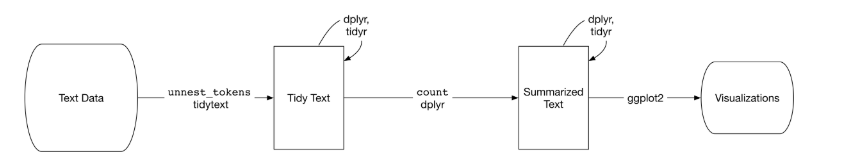
\includegraphics[width=475px]{tidytext} \caption{Flowchart of a Typical Tidy Text Analysis (Silge \& Robinson)}\label{fig:unnamed-chunk-12}
\end{figure}
To begin, we created a data frame containing only the words of the
tweets. This is done by first selecting two columns: the status id,
which are unique identifiers for each tweet, and the full text column.
From there, we use the \texttt{unnest\_token()} function from the
\texttt{tidytext} package to split the text column into words and create
a row for each word of each tweet.

\small
\begin{Shaded}
\begin{Highlighting}[]
\NormalTok{words <-}\StringTok{ }\NormalTok{tweets_final }\OperatorTok\StringTok{ }
\StringTok{    }\NormalTok{dplyr}\OperatorTok{::}\KeywordTok{select}\NormalTok{(status_id, full_text_low) }\OperatorTok\StringTok{ }
\StringTok{    }\KeywordTok{unnest_tokens}\NormalTok{(word, full_text_low)}
\end{Highlighting}
\end{Shaded}
\normalsize

For both of the analyses, only certain words are of interest, especially
when adding sentiment or determining which words are the most common.
Other words, such as ``and'', ``is'', and ``the'', are known as stop
words and are filtered out. A stop words lexicon can be accessed through
the \texttt{tidytext} package by using the function
\texttt{get\_stopwords()}. Once the stop words data frame is loaded into
the environment, we added additional rows for ``words'' that are common
to tweets but are unnecessary for the environment. After the words and
stop words data sets were created, the stop words data set was
\texttt{anti\_joined} to the words data set to filter those words out.
From there, simple natural language processing such as determining most
common words were possible. Examples are shown in Table
\ref{tab:tweetwords}.

\small
\begin{Shaded}
\begin{Highlighting}[]
\CommentTok{#specifying stop words}
\NormalTok{my_stop_words <-}\StringTok{ }\NormalTok{stop_words }\OperatorTok\StringTok{ }
\StringTok{    }\NormalTok{dplyr}\OperatorTok{::}\KeywordTok{select}\NormalTok{(}\OperatorTok{-}\NormalTok{lexicon) }\OperatorTok\StringTok{ }
\StringTok{    }\CommentTok{#adding common stop words from Twitter}
\StringTok{    }\KeywordTok{bind_rows}\NormalTok{(}\KeywordTok{tibble}\NormalTok{(}\DataTypeTok{word =} \KeywordTok{c}\NormalTok{(}\StringTok{"https"}\NormalTok{, }\StringTok{"t.co"}\NormalTok{, }\StringTok{"rt"}\NormalTok{, }\StringTok{"amp"}\NormalTok{,}
                              \StringTok{"4yig9gzh5t"}\NormalTok{,}\StringTok{"fyy2ceydhi"}\NormalTok{,}
                              \StringTok{"78"}\NormalTok{,}\StringTok{"fakenews"}\NormalTok{, }\StringTok{"na"}\NormalTok{)))}

\CommentTok{#removing stop words}
\NormalTok{tweet_words <-}\StringTok{ }\NormalTok{words }\OperatorTok\StringTok{ }
\StringTok{    }\KeywordTok{anti_join}\NormalTok{(my_stop_words)}
\end{Highlighting}
\end{Shaded}
\normalsize
\begin{table}[!h]

\caption[Examples of Tweet Words Data Frame]{\label{tab:tweetwords}Examples of Tweet Words Data Frame}
\centering
\begin{tabular}{l|l}
\hline
Status ID & Word\\
\hline
1092188777672556546 & edelman11\\
\hline
1092188777672556546 & field\\
\hline
1092188777672556546 & u6eikf89gy\\
\hline
1092188685670395904 & calm\\
\hline
1092188685670395904 & cool\\
\hline
1092188685670395904 & collected\\
\hline
1092188685670395904 & jaredgoff16\\
\hline
1092188685670395904 & ready\\
\hline
1092188685670395904 & sbliii\\
\hline
1092188685670395904 & mikesilver\\
\hline
\end{tabular}
\end{table}
An additional step was necessary to add sentiments to these words. The
\texttt{tidytext} package includes three lexicons containing words and
their corresponding sentiments. The three include \texttt{AFINN} from
Nielsen (2011), \texttt{bing} from Hu \& Liu (2004), and \texttt{nrc}
from Mohammad \& Turney (2013). The first assigns words with a number
from -5 to 5, with 5 being the most positive words and -5 being the most
negative words. The second simply assigns words as positive or negative.
The third assigns words in a binary fashion into the categories of
positive, negative, anger, anticipation, disgust, fear, joy, sadness,
surprise, and trust. For simplicity of determining negativity, we are
using the \texttt{bing} lexicon. For simple counts of sentiment across
the whole tweets data set, we simply join the \texttt{bing} lexicon to
the words data set. Examples are shown in Table \ref{tab:sentiments}.

\small
\begin{Shaded}
\begin{Highlighting}[]
\CommentTok{#getting sentiments- using bing}
\NormalTok{  bing_lex <-}\StringTok{ }\KeywordTok{get_sentiments}\NormalTok{(}\StringTok{"bing"}\NormalTok{)}

\CommentTok{#joining words with the sentiments}
\NormalTok{full_sentiments <-}\StringTok{ }\NormalTok{tweet_words }\OperatorTok
\StringTok{  }\KeywordTok{left_join}\NormalTok{(bing_lex)}
\end{Highlighting}
\end{Shaded}
\normalsize
\begin{table}[!h]

\caption[Examples of Tweet Words with Sentiment Data Frame]{\label{tab:sentiments}Examples of Tweet Words with Sentiment Data Frame}
\centering
\begin{tabular}{l|l|l}
\hline
Status ID & Word & Sentiment\\
\hline
1092188777672556546 & edelman11 & NA\\
\hline
1092188777672556546 & field & NA\\
\hline
1092188777672556546 & u6eikf89gy & NA\\
\hline
1092188685670395904 & calm & positive\\
\hline
1092188685670395904 & cool & positive\\
\hline
1092188685670395904 & collected & NA\\
\hline
1092188685670395904 & jaredgoff16 & NA\\
\hline
1092188685670395904 & ready & positive\\
\hline
1092188685670395904 & sbliii & NA\\
\hline
1092188685670395904 & mikesilver & NA\\
\hline
\end{tabular}
\end{table}
\subsection{Sentiment Analysis by
Player}\label{sentiment-analysis-by-player}

Given our interest in the differences in sentiments for players
depending on demographic information, we needed to change the format of
our data in order to determine the sentiment for each player
individually. To do so, we wrote a function called
\texttt{add\_sentiments} that takes an integer as an argument. Within
the function, we filter the \texttt{tweets\_final} data frame to match
the indexed name. From there, the same process as above of unnesting the
tweets by words, filtering out stop words, then joining to the sentiment
lexicon is employed. Lastly, we want the data to be formatted in a data
frame containing a single row with three columns. One column is the name
of the player and the two others are the counts of negative and positive
words. This data frame is returned by the function. In order to
determine the sentiments of all 50 starting players, we use the
\texttt{map\_df()} function of the \texttt{purrr} package (Henry \&
Wickham, 2019). This function takes a list from 1 to 50 as the first
arguments and the function name as the second. By running
\texttt{map\_df()}, we effectively run our function for all 50 players.
This results in a data set of 50 rows and three columns that containes
the counts of positive and negative words for each player.

\small
\begin{Shaded}
\begin{Highlighting}[]
\CommentTok{#list of names for loop}
\NormalTok{names <-}\StringTok{ }\KeywordTok{as.list}\NormalTok{(starters_clean}\OperatorTok{$}\NormalTok{name_clean)}

\CommentTok{#index for the 5 names}
\NormalTok{index <-}\StringTok{ }\KeywordTok{as.list}\NormalTok{(}\DecValTok{1}\OperatorTok{:}\KeywordTok{length}\NormalTok{(names))}

\CommentTok{#writing function}
\NormalTok{add_sentiments <-}\StringTok{ }\ControlFlowTok{function}\NormalTok{(i) \{}
  
  \CommentTok{#filter for the person}
\NormalTok{  tweets <-}\StringTok{ }\NormalTok{tweets_final }\OperatorTok
\StringTok{    }\KeywordTok{filter}\NormalTok{(name_clean_final }\OperatorTok{==}\StringTok{ }\NormalTok{names[i])}
  
  \CommentTok{#pick out words}
\NormalTok{  words <-}\StringTok{ }\NormalTok{tweets }\OperatorTok\StringTok{ }
\StringTok{    }\NormalTok{dplyr}\OperatorTok{::}\KeywordTok{select}\NormalTok{(status_id, full_text_low) }\OperatorTok\StringTok{ }
\StringTok{    }\KeywordTok{unnest_tokens}\NormalTok{(word, full_text_low)}
  
  \CommentTok{#creating df of stop words  }
\NormalTok{  my_stop_words <-}\StringTok{ }\NormalTok{stop_words }\OperatorTok\StringTok{ }
\StringTok{    }\NormalTok{dplyr}\OperatorTok{::}\KeywordTok{select}\NormalTok{(}\OperatorTok{-}\NormalTok{lexicon) }\OperatorTok\StringTok{ }
\StringTok{    }\KeywordTok{bind_rows}\NormalTok{(}\KeywordTok{data.frame}\NormalTok{(}\DataTypeTok{word =} \KeywordTok{c}\NormalTok{(}\StringTok{"https"}\NormalTok{, }\StringTok{"t.co"}\NormalTok{, }\StringTok{"rt"}\NormalTok{, }\StringTok{"amp"}\NormalTok{,}
                                  \StringTok{"4yig9gzh5t"}\NormalTok{,}\StringTok{"fyy2ceydhi"}\NormalTok{,}
                                  \StringTok{"78"}\NormalTok{,}\StringTok{"fakenews"}\NormalTok{)))}

  \CommentTok{#anti-join with stop words to filter those words out}
\NormalTok{  tweet_words <-}\StringTok{ }\NormalTok{words }\OperatorTok\StringTok{ }
\StringTok{    }\KeywordTok{anti_join}\NormalTok{(my_stop_words)}
  
  \CommentTok{#getting sentiments}
\NormalTok{  bing_lex <-}\StringTok{ }\KeywordTok{get_sentiments}\NormalTok{(}\StringTok{"bing"}\NormalTok{)}

  \CommentTok{#joining sentiments with non-stop words from tweets}
\NormalTok{  fn_sentiment <-}\StringTok{ }\NormalTok{tweet_words }\OperatorTok\StringTok{ }
\StringTok{    }\KeywordTok{left_join}\NormalTok{(bing_lex) }
  
  \CommentTok{#creating df with n of sentiments}
\NormalTok{  df <-}\StringTok{ }\NormalTok{fn_sentiment }\OperatorTok\StringTok{ }
\StringTok{    }\KeywordTok{filter}\NormalTok{(}\OperatorTok{!}\KeywordTok{is.na}\NormalTok{(sentiment)) }\OperatorTok\StringTok{ }
\StringTok{    }\KeywordTok{group_by}\NormalTok{(sentiment) }\OperatorTok\StringTok{ }
\StringTok{    }\KeywordTok{summarise}\NormalTok{(}\DataTypeTok{n=}\KeywordTok{n}\NormalTok{())}
  
  \CommentTok{#making 1 row df of name and sentiment counts}
\NormalTok{  df_}\DecValTok{2}\NormalTok{ <-}\StringTok{ }\NormalTok{df }\OperatorTok
\StringTok{  }\KeywordTok{mutate}\NormalTok{(}\DataTypeTok{player =}\NormalTok{ names[i]) }\OperatorTok
\StringTok{  }\KeywordTok{spread}\NormalTok{(}\DataTypeTok{key =}\NormalTok{ sentiment, }\DataTypeTok{value =}\NormalTok{ n)}

  \KeywordTok{return}\NormalTok{(df_}\DecValTok{2}\NormalTok{)}
  
\NormalTok{\}}

\CommentTok{#stacking sentiments for each player}
\NormalTok{sentiments_full <-}\StringTok{ }\KeywordTok{map_df}\NormalTok{(index, add_sentiments)}
\end{Highlighting}
\end{Shaded}
\normalsize

This data set named \texttt{sentiments\_full} is then joined to the
initial starters data set to match the sentiment counts to other
demographic data. We create other variables including the total
sentiment words (by adding the negative and positive counts), the
percent of negative words (by dividing the negative count column by the
total column), and the percent of positive words (by dividing the
positive count column by the total column). Examples are shown in Table
\ref{tab:percentages}.

\small
\begin{Shaded}
\begin{Highlighting}[]
\CommentTok{#joining and creating percentages}
\NormalTok{starters_sentiment <-}\StringTok{ }\NormalTok{starters_clean }\OperatorTok
\StringTok{  }\KeywordTok{left_join}\NormalTok{(sentiments_full, }\DataTypeTok{by =} \KeywordTok{c}\NormalTok{(}\StringTok{"name_clean"}\NormalTok{ =}\StringTok{ "player"}\NormalTok{)) }\OperatorTok
\StringTok{  }\KeywordTok{mutate}\NormalTok{(}\DataTypeTok{totalsentiment =}\NormalTok{ positive}\OperatorTok{+}\NormalTok{negative,}
         \DataTypeTok{neg_perc =} \KeywordTok{round}\NormalTok{(negative}\OperatorTok{/}\NormalTok{totalsentiment }\OperatorTok{*}\StringTok{ }\DecValTok{100}\NormalTok{, }\DecValTok{2}\NormalTok{),}
         \DataTypeTok{pos_perc =} \KeywordTok{round}\NormalTok{(positive}\OperatorTok{/}\NormalTok{totalsentiment }\OperatorTok{*}\StringTok{ }\DecValTok{100}\NormalTok{, }\DecValTok{2}\NormalTok{)) }
\end{Highlighting}
\end{Shaded}
\normalsize
\begin{table}[!h]

\caption[Examples from Starters Data Frame with Sentiment Percentages]{\label{tab:percentages}Examples from Starters Data Frame with Sentiment Percentages}
\centering
\begin{tabular}{>{\raggedright\arraybackslash}p{2cm}|>{\raggedright\arraybackslash}p{2cm}|>{\raggedright\arraybackslash}p{2cm}|>{\raggedleft\arraybackslash}p{2cm}|>{\raggedleft\arraybackslash}p{2cm}|>{\raggedleft\arraybackslash}p{2cm}}
\hline
Name & Race & Position & Total Number of Tweets & \% of Neg Tweets & \% of Pos Tweets\\
\hline
jared goff & white & QB & 54817 & 54.15 & 45.85\\
\hline
todd gurley & black & RB & 24352 & 53.12 & 46.88\\
\hline
brandin cooks & black & WR & 7473 & 50.06 & 49.94\\
\hline
\end{tabular}
\end{table}
From here, we create visualizations comparing average negative and
positive percentages across different groups, including race, team, and
position.

\section{Results}\label{results}

\subsection{What were the most popular
words?}\label{what-were-the-most-popular-words}

In total, 618,628 tweets with 652,411 individual player mentions are
gathered for the 50 starting players during the 7-hour specified period.

The 20 words that are used the most often (after removing stop words)
are shown below.

\small
\begin{Shaded}
\begin{Highlighting}[]
\CommentTok{#word counts}
\NormalTok{word_counts <-}\StringTok{ }\NormalTok{tweet_words }\OperatorTok
\StringTok{  }\KeywordTok{count}\NormalTok{(word, }\DataTypeTok{sort =} \OtherTok{TRUE}\NormalTok{)}

\CommentTok{#viz}
\KeywordTok{ggplot}\NormalTok{(word_counts }\OperatorTok\StringTok{ }\KeywordTok{head}\NormalTok{(}\DataTypeTok{n =}\NormalTok{ 20L), }
       \KeywordTok{aes}\NormalTok{(}\KeywordTok{reorder}\NormalTok{(word, n), n)) }\OperatorTok{+}
\StringTok{  }\KeywordTok{geom_col}\NormalTok{() }\OperatorTok{+}
\StringTok{  }\KeywordTok{xlab}\NormalTok{(}\OtherTok{NULL}\NormalTok{) }\OperatorTok{+}
\StringTok{  }\KeywordTok{ylab}\NormalTok{(}\StringTok{"Counts"}\NormalTok{) }\OperatorTok{+}
\StringTok{  }\KeywordTok{scale_y_continuous}\NormalTok{(}\DataTypeTok{labels =}\NormalTok{ comma) }\OperatorTok{+}
\StringTok{  }\KeywordTok{coord_flip}\NormalTok{() }\OperatorTok{+}
\StringTok{  }\KeywordTok{theme_classic}\NormalTok{()}
\end{Highlighting}
\end{Shaded}
\begin{figure}
\centering
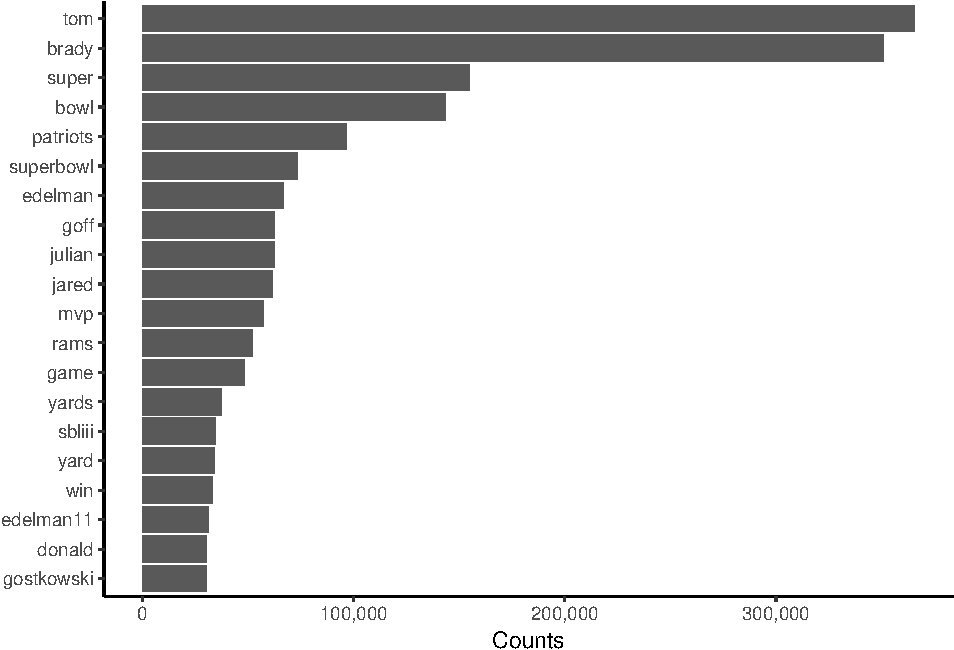
\includegraphics{thesis_files/figure-latex/popular-1.pdf}
\caption{\label{fig:popular}Top 20 Most Popular Words}
\end{figure}
\normalsize
In Figure \ref{fig:popular}, the top four most popular words are
``tom'', ``brady'', ``super'', and ``bowl''. Of the 20 top words, 9 are
names of players. We then determine the 20 top words without names by
adding the list of full names and twitter handles to our stop words data
set. Those words are below.

\small
\begin{Shaded}
\begin{Highlighting}[]
\CommentTok{#viz}
\KeywordTok{ggplot}\NormalTok{(word_counts }\OperatorTok\StringTok{ }\KeywordTok{head}\NormalTok{(}\DataTypeTok{n =}\NormalTok{ 20L), }
       \KeywordTok{aes}\NormalTok{(}\KeywordTok{reorder}\NormalTok{(word, n), n)) }\OperatorTok{+}
\StringTok{  }\KeywordTok{geom_col}\NormalTok{() }\OperatorTok{+}
\StringTok{  }\KeywordTok{xlab}\NormalTok{(}\OtherTok{NULL}\NormalTok{) }\OperatorTok{+}
\StringTok{  }\KeywordTok{ylab}\NormalTok{(}\StringTok{"Counts"}\NormalTok{) }\OperatorTok{+}
\StringTok{  }\KeywordTok{scale_y_continuous}\NormalTok{(}\DataTypeTok{labels =}\NormalTok{ comma) }\OperatorTok{+}
\StringTok{  }\KeywordTok{coord_flip}\NormalTok{() }\OperatorTok{+}
\StringTok{  }\KeywordTok{theme_classic}\NormalTok{()}
\end{Highlighting}
\end{Shaded}
\begin{figure}
\centering
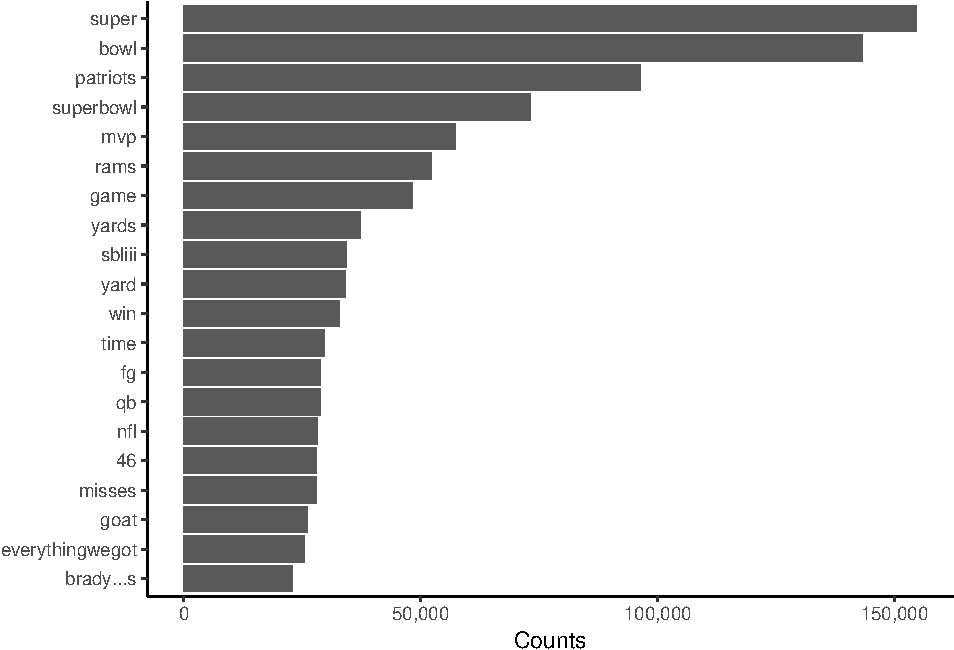
\includegraphics{thesis_files/figure-latex/popnonames-1.pdf}
\caption{\label{fig:popnonames}Top 20 Most Popular Words without Names}
\end{figure}
\normalsize
In Figure \ref{fig:popnonames}, the top four most popular words are
``super'', ``bowl'', ``patriots'', and ``superbowl''.

\subsection{Who had the most tweets from the
Patriots?}\label{who-had-the-most-tweets-from-the-patriots}

\small
\begin{Shaded}
\begin{Highlighting}[]
\CommentTok{#number of tweets for each player on NE}
\KeywordTok{ggplot}\NormalTok{(starters_sent_n }\OperatorTok\StringTok{ }
\StringTok{         }\KeywordTok{filter}\NormalTok{(team }\OperatorTok{==}\StringTok{ "NE"}\NormalTok{),}
       \KeywordTok{aes}\NormalTok{(}\KeywordTok{reorder}\NormalTok{(name_clean, n), n}\OperatorTok{/}\DecValTok{2}\NormalTok{)) }\OperatorTok{+}
\StringTok{  }\KeywordTok{geom_col}\NormalTok{() }\OperatorTok{+}
\StringTok{  }\KeywordTok{xlab}\NormalTok{(}\OtherTok{NULL}\NormalTok{) }\OperatorTok{+}
\StringTok{  }\KeywordTok{ylab}\NormalTok{(}\StringTok{"Number of Tweets"}\NormalTok{) }\OperatorTok{+}
\StringTok{  }\KeywordTok{scale_y_continuous}\NormalTok{(}\DataTypeTok{labels =}\NormalTok{ comma) }\OperatorTok{+}
\StringTok{  }\KeywordTok{coord_flip}\NormalTok{() }\OperatorTok{+}
\StringTok{  }\KeywordTok{theme_classic}\NormalTok{()}
\end{Highlighting}
\end{Shaded}
\begin{figure}
\centering
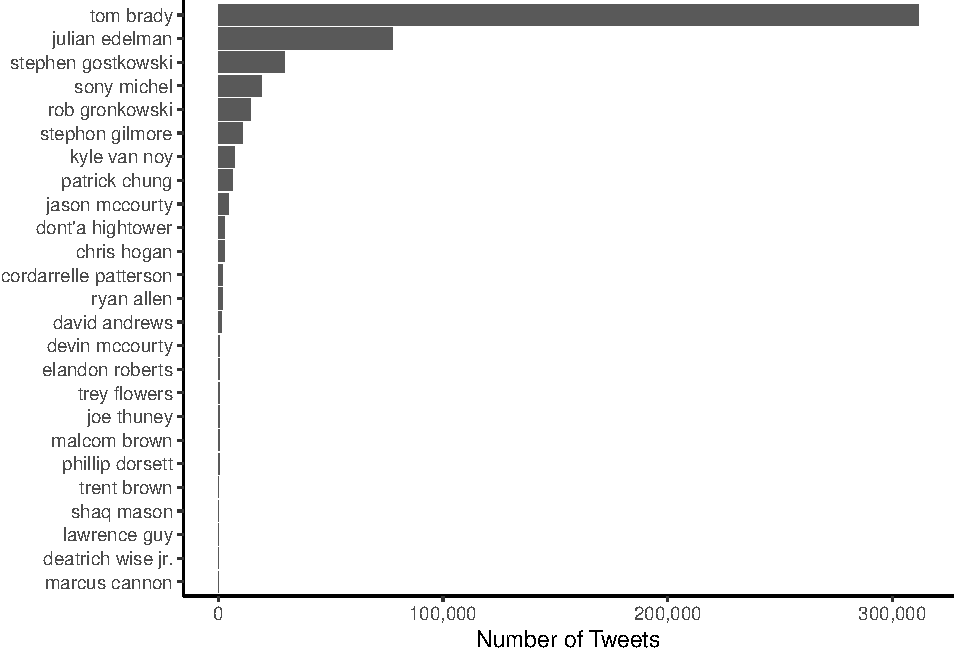
\includegraphics{thesis_files/figure-latex/tweetspats-1.pdf}
\caption{\label{fig:tweetspats}Number of Tweets per Patriots Player}
\end{figure}
\normalsize
In Figure \ref{fig:tweetspats}, The players with the most tweets are Tom
Brady, Julian Edelman, Stephen Gostkowski, Sony Michel, and Rob
Gronkowski. Tom Brady is the star quarterback for the Patriots. As the
quarterback, most plays revolve around his actions. Julian Edelman is a
wide receiver and was named the MVP of Super Bowl LIII. Stephen
Gostkowski is the kicker. The kicker's performance, especially in a
Super Bowl, is important as the three points from a field goal can make
or break the game outcome. Sony Michel is a running back and Rob
Gronkowski is the Patriot's popular tight end. The position of these
players leads them to have a lot of contact with the ball throughout the
game. Quite a few players had so few tweets compared to the top few
players that it cannot be determined from this visualization the exact
number of tweets each player had. Table \ref{tab:tweetspatst} includes
the players with more than 700 tweet references, their position, race,
and number of tweets.

\small
\begin{table}[!h]

\caption[Number of Tweets per Patriots Player]{\label{tab:tweetspatst}Number of Tweets per Patriots Player}
\centering
\begin{tabular}{l|l|l|l|r}
\hline
Name & Position & Position group & Race & Number of tweets\\
\hline
tom brady & QB & O & white & 311496\\
\hline
julian edelman & WR & O & white & 77413\\
\hline
stephen gostkowski & K & S & white & 29453\\
\hline
sony michel & RB & O & black & 19428\\
\hline
rob gronkowski & TE & O & white & 14361\\
\hline
stephon gilmore & CB & D & black & 11023\\
\hline
kyle van noy & OLB & D & black & 7398\\
\hline
patrick chung & SS & D & black & 6349\\
\hline
jason mccourty & CB & D & black & 4495\\
\hline
dont'a hightower & OLB & D & black & 2856\\
\hline
chris hogan & WR & O & white & 2835\\
\hline
cordarrelle patterson & KR & S & black & 2003\\
\hline
ryan allen & P & S & white & 1921\\
\hline
david andrews & C & O & white & 1390\\
\hline
devin mccourty & FS & D & black & 777\\
\hline
elandon roberts & MLB & D & black & 716\\
\hline
\end{tabular}
\end{table}
\normalsize

\subsection{Who had the most tweets from the
Rams?}\label{who-had-the-most-tweets-from-the-rams}

\small
\begin{Shaded}
\begin{Highlighting}[]
\CommentTok{#number of tweets for each player on LA}
\KeywordTok{ggplot}\NormalTok{(starters_sent_n }\OperatorTok\StringTok{ }
\StringTok{         }\KeywordTok{filter}\NormalTok{(team }\OperatorTok{==}\StringTok{ "LA"}\NormalTok{),}
       \KeywordTok{aes}\NormalTok{(}\KeywordTok{reorder}\NormalTok{(name_clean, n), n}\OperatorTok{/}\DecValTok{2}\NormalTok{)) }\OperatorTok{+}
\StringTok{  }\KeywordTok{geom_col}\NormalTok{() }\OperatorTok{+}
\StringTok{  }\KeywordTok{xlab}\NormalTok{(}\OtherTok{NULL}\NormalTok{) }\OperatorTok{+}
\StringTok{  }\KeywordTok{ylab}\NormalTok{(}\StringTok{"Number of Tweets"}\NormalTok{) }\OperatorTok{+}
\StringTok{  }\KeywordTok{scale_y_continuous}\NormalTok{(}\DataTypeTok{labels =}\NormalTok{ comma) }\OperatorTok{+}
\StringTok{  }\KeywordTok{coord_flip}\NormalTok{() }\OperatorTok{+}
\StringTok{  }\KeywordTok{theme_classic}\NormalTok{()}
\end{Highlighting}
\end{Shaded}
\begin{figure}
\centering
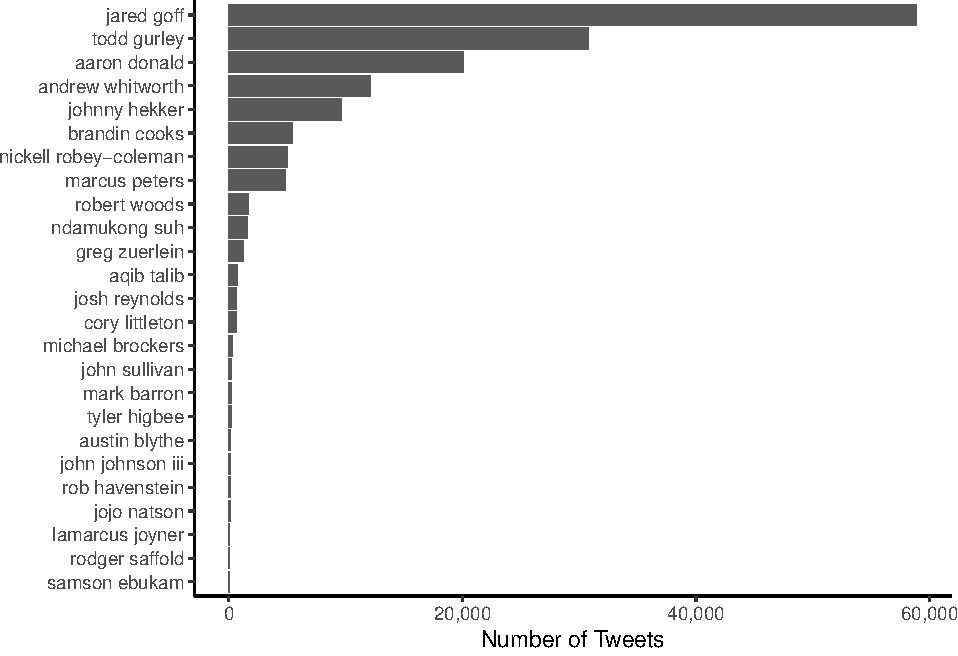
\includegraphics{thesis_files/figure-latex/tweetsrams-1.pdf}
\caption{\label{fig:tweetsrams}Number of Tweets per Rams Player}
\end{figure}
\normalsize
In Figure \ref{fig:tweetsrams}, the players with the most tweets are
Jared Goff, Todd Gurley, Aaron Donald, Andrew Witworth, and Johnny
Hekker. Those first two players are the quarterback and leading running
back, respectively. Aaron Donald is a defensive tackle, Andrew Witworth
is an offensive tackle, and Johnny Hekker is the punter. Unlike with the
Patriots, these players are not necessarily those who would have the
most contact with the ball but all are considered top players for the
Rams. Again, the number of tweets for many players cannot be determined
based on this visualization. Below is another table of the players with
more than 700 tweet references, their demographic information, and
number of tweets.

\small
\begin{table}[!h]

\caption[Number of Tweets per Rams Player]{\label{tab:tweetsramst}Number of Tweets per Rams Player}
\centering
\begin{tabular}{l|l|l|l|r}
\hline
Name & Position & Position group & Race & Number of tweets\\
\hline
jared goff & QB & O & white & 58900\\
\hline
todd gurley & RB & O & black & 30833\\
\hline
aaron donald & RE & D & black & 20068\\
\hline
andrew whitworth & LT & O & white & 12171\\
\hline
johnny hekker & P & S & white & 9638\\
\hline
brandin cooks & WR & O & black & 5481\\
\hline
nickell robey-coleman & CB & D & black & 5039\\
\hline
marcus peters & CB & D & black & 4838\\
\hline
robert woods & WR & O & black & 1691\\
\hline
ndamukong suh & NT & D & black & 1594\\
\hline
greg zuerlein & K & S & white & 1227\\
\hline
aqib talib & CB & D & black & 769\\
\hline
\end{tabular}
\end{table}
\normalsize

A few observations from Tables \ref{tab:tweetspatst} and
\ref{tab:tweetsramst} are that the player with the most tweets on both
teams is the quarterback and a majority of the players in the top 5 are
offensive players. In addition, we note that the distribution of tweets
across both teams appears to somewhat follow a Zipf's distribution,
which states that the probability of attaining a certain \(x\) is
proportional to \(x^{-t}\), where \(t >= 1\). This law is commonly used
in studies of word frequencies.

\subsection{Which team has a higher negative sentiment
percentage?}\label{which-team-has-a-higher-negative-sentiment-percentage}

Although no formal hypotheses are made in this study, we expect that the
team that loses will see a higher average negative sentiment percentage.
Therefore, we expect the Rams, who lost, to have a higher average
negative sentiment compared to the Patriots. This is tested
directionally and no models are fit and no statistical inference tests
are performed.

\small
\begin{Shaded}
\begin{Highlighting}[]
\CommentTok{#sentiments by team}
\KeywordTok{ggplot}\NormalTok{(starter_sent_}\DecValTok{2}\NormalTok{, }\KeywordTok{aes}\NormalTok{(}\DataTypeTok{x =}\NormalTok{ sentiment, }\DataTypeTok{y =}\NormalTok{ mean_perc_sent)) }\OperatorTok{+}
\StringTok{  }\KeywordTok{geom_bar}\NormalTok{(}\DataTypeTok{stat =} \StringTok{"identity"}\NormalTok{, }\DataTypeTok{position =} \StringTok{"dodge"}\NormalTok{, }\DataTypeTok{color =} \StringTok{"black"}\NormalTok{) }\OperatorTok{+}
\StringTok{  }\KeywordTok{theme}\NormalTok{(}\DataTypeTok{axis.text.x =} \KeywordTok{element_text}\NormalTok{(}\DataTypeTok{angle =} \DecValTok{45}\NormalTok{, }\DataTypeTok{hjust =} \DecValTok{1}\NormalTok{)) }\OperatorTok{+}\StringTok{ }
\StringTok{  }\KeywordTok{facet_wrap}\NormalTok{(}\OperatorTok{~}\NormalTok{team, }\DataTypeTok{ncol =} \DecValTok{2}\NormalTok{) }\OperatorTok{+}
\StringTok{  }\KeywordTok{ylab}\NormalTok{(}\StringTok{"Average Negative Percentage"}\NormalTok{) }\OperatorTok{+}
\StringTok{  }\KeywordTok{geom_label}\NormalTok{(}\KeywordTok{aes}\NormalTok{(}\DataTypeTok{label =} \KeywordTok{round}\NormalTok{(mean_perc_sent, }\DecValTok{0}\NormalTok{))) }\OperatorTok{+}
\StringTok{  }\KeywordTok{theme}\NormalTok{(}\DataTypeTok{axis.text.x =} \KeywordTok{element_blank}\NormalTok{(), }
        \DataTypeTok{axis.ticks.x =} \KeywordTok{element_blank}\NormalTok{(), }
        \DataTypeTok{axis.title.x =} \KeywordTok{element_blank}\NormalTok{())}
\end{Highlighting}
\end{Shaded}
\begin{figure}
\centering
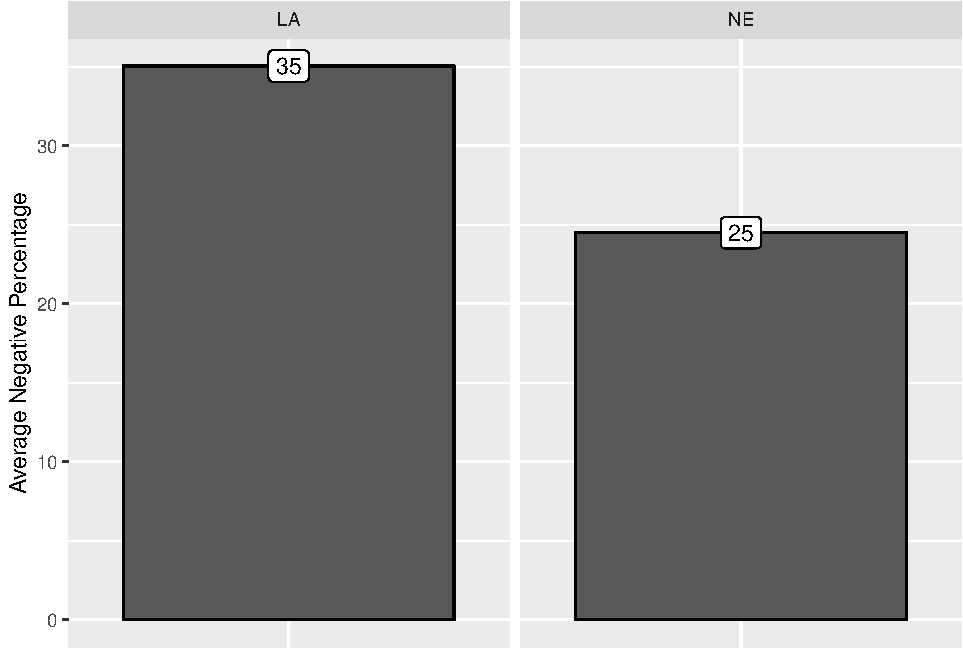
\includegraphics{thesis_files/figure-latex/unnamed-chunk-25-1.pdf}
\caption{\label{fig:unnamed-chunk-25}Average Negative Sentiment Percentage
by Team}
\end{figure}
\normalsize
Our data matches this expectation. The average negative sentiment
percentage for the Rams is 35\% while the average negative sentiment for
the Patriots is 25\%.

\subsection{Which racial group had a higher average negative sentiment
percentage?}\label{which-racial-group-had-a-higher-average-negative-sentiment-percentage}

We want to see if there appear to be directional differences in the mean
negative sentiments for black players and white players. This is
explored across all players, and then explored within teams, given that
the rams have overall more negative sentiment.

\small
\begin{Shaded}
\begin{Highlighting}[]
\CommentTok{#sentiments by race}
\KeywordTok{ggplot}\NormalTok{(starter_sent_}\DecValTok{2}\NormalTok{, }\KeywordTok{aes}\NormalTok{(}\DataTypeTok{x =}\NormalTok{ sentiment, }\DataTypeTok{y =}\NormalTok{ mean_perc_sent, }
                           \DataTypeTok{fill =}\NormalTok{ Race)) }\OperatorTok{+}
\StringTok{  }\KeywordTok{geom_bar}\NormalTok{(}\DataTypeTok{stat =} \StringTok{"identity"}\NormalTok{, }\DataTypeTok{position =} \StringTok{"dodge"}\NormalTok{, }\DataTypeTok{color =} \StringTok{"black"}\NormalTok{) }\OperatorTok{+}
\StringTok{  }\KeywordTok{theme}\NormalTok{(}\DataTypeTok{axis.text.x =} \KeywordTok{element_text}\NormalTok{(}\DataTypeTok{angle =} \DecValTok{45}\NormalTok{, }\DataTypeTok{hjust =} \DecValTok{1}\NormalTok{)) }\OperatorTok{+}
\StringTok{  }\KeywordTok{scale_fill_manual}\NormalTok{(}\DataTypeTok{values=}\KeywordTok{c}\NormalTok{(}\StringTok{"black"}\NormalTok{, }\StringTok{"white"}\NormalTok{)) }\OperatorTok{+}
\StringTok{  }\KeywordTok{ylab}\NormalTok{(}\StringTok{"Average Negative Percentage"}\NormalTok{) }\OperatorTok{+}
\StringTok{  }\KeywordTok{theme}\NormalTok{(}\DataTypeTok{axis.text.x =} \KeywordTok{element_blank}\NormalTok{(), }
        \DataTypeTok{axis.ticks.x =} \KeywordTok{element_blank}\NormalTok{(), }
        \DataTypeTok{axis.title.x =} \KeywordTok{element_blank}\NormalTok{())}
\end{Highlighting}
\end{Shaded}
\begin{figure}
\centering
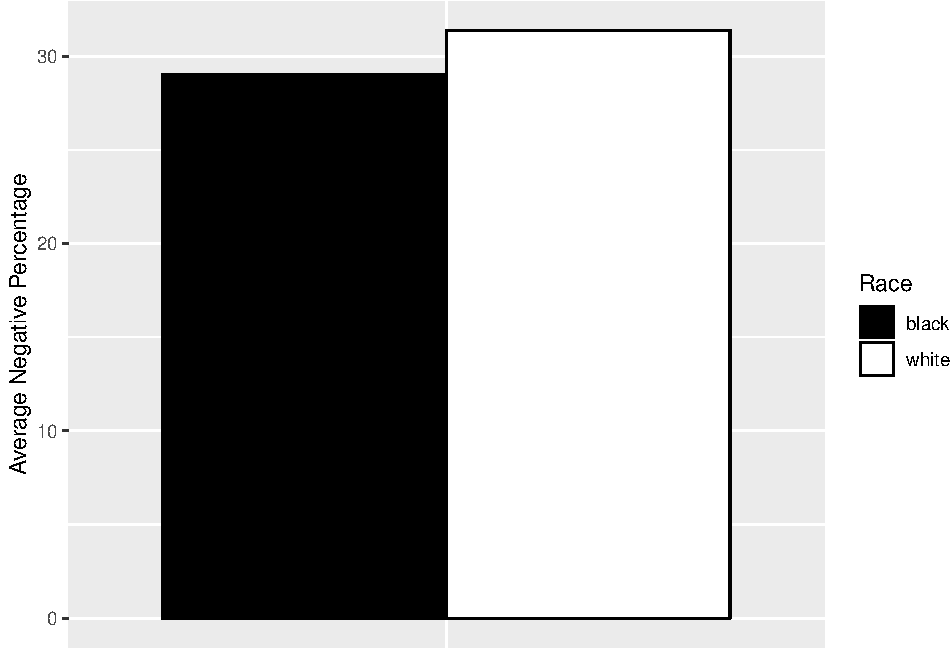
\includegraphics{thesis_files/figure-latex/raceneg-1.pdf}
\caption{\label{fig:raceneg}Average Negative Words Percentage by Race}
\end{figure}
\normalsize

From \ref{fig:raceneg}, we can see that white players have higher
average percentage of negative words across both teams.

\small
\begin{Shaded}
\begin{Highlighting}[]
\CommentTok{#sentiments by race and team}
\KeywordTok{ggplot}\NormalTok{(starter_sent_}\DecValTok{2}\NormalTok{, }\KeywordTok{aes}\NormalTok{(}\DataTypeTok{x =}\NormalTok{ sentiment, }\DataTypeTok{y =}\NormalTok{ mean_perc_sent, }
                           \DataTypeTok{fill =}\NormalTok{ Race)) }\OperatorTok{+}
\StringTok{  }\KeywordTok{geom_bar}\NormalTok{(}\DataTypeTok{stat =} \StringTok{"identity"}\NormalTok{, }\DataTypeTok{position =} \StringTok{"dodge"}\NormalTok{, }\DataTypeTok{color =} \StringTok{"black"}\NormalTok{) }\OperatorTok{+}
\StringTok{  }\KeywordTok{theme}\NormalTok{(}\DataTypeTok{axis.text.x =} \KeywordTok{element_text}\NormalTok{(}\DataTypeTok{angle =} \DecValTok{45}\NormalTok{, }\DataTypeTok{hjust =} \DecValTok{1}\NormalTok{)) }\OperatorTok{+}
\StringTok{  }\KeywordTok{scale_fill_manual}\NormalTok{(}\DataTypeTok{values=}\KeywordTok{c}\NormalTok{(}\StringTok{"black"}\NormalTok{, }\StringTok{"white"}\NormalTok{)) }\OperatorTok{+}\StringTok{ }
\StringTok{  }\KeywordTok{facet_wrap}\NormalTok{(}\OperatorTok{~}\NormalTok{team, }\DataTypeTok{ncol =} \DecValTok{2}\NormalTok{) }\OperatorTok{+}
\StringTok{  }\KeywordTok{ylab}\NormalTok{(}\StringTok{"Average Negative Percentage"}\NormalTok{) }\OperatorTok{+}
\StringTok{  }\KeywordTok{theme}\NormalTok{(}\DataTypeTok{axis.text.x =} \KeywordTok{element_blank}\NormalTok{(), }
        \DataTypeTok{axis.ticks.x =} \KeywordTok{element_blank}\NormalTok{(), }
        \DataTypeTok{axis.title.x =} \KeywordTok{element_blank}\NormalTok{())}
\end{Highlighting}
\end{Shaded}
\begin{figure}
\centering
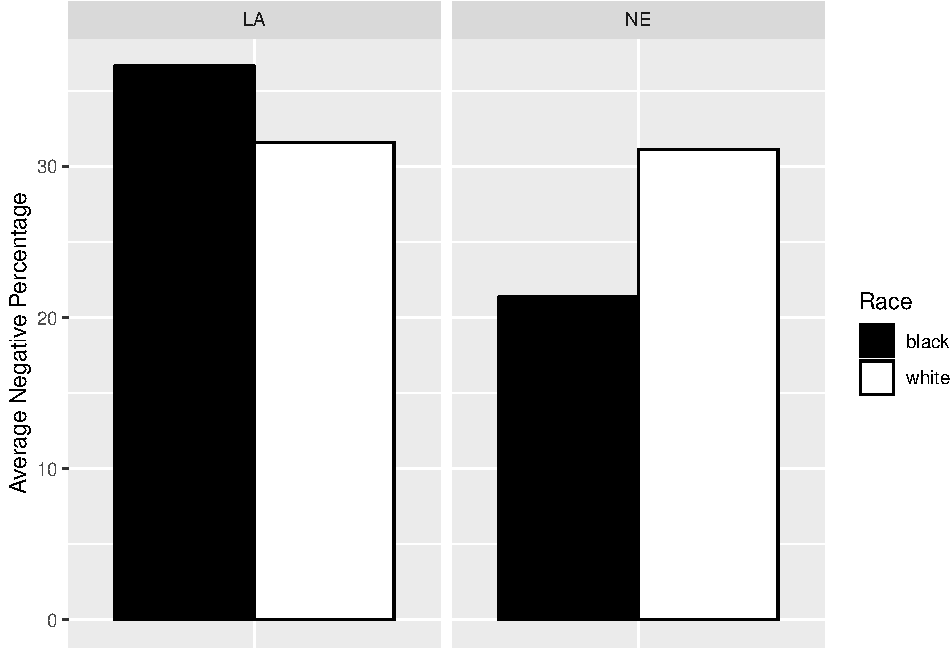
\includegraphics{thesis_files/figure-latex/raceteamneg-1.pdf}
\caption{\label{fig:raceteamneg}Average Negative Words by Race and Team}
\end{figure}
\normalsize
When split by team, we see a higher average negative sentiment
percentage for black players on the Rams and for white players on the
Patriots. This empirical finding presages our more rigourous hypothesis
in the next chapter.

\section{Conclusions and Moving
Forward}\label{conclusions-and-moving-forward}

There are a few basic conclusions and observations to be made regarding
the results of our first study. First, in regards to the top words, many
did not have sentiments attached to them because they are specific to
football. For example, one of the words in the top 20 is ``goat''. This
is a word often used when describing Tom Brady. Technically, it is an
acronym and stands for ``greatest of all time''. This common word is
quite positive however it is not included in the sentiment lexicon.
Other words that are specific to football that need to be added to the
lexicon as positive words when in a football context are ``history'',
``ring'', ``rings'', ``dynasty'', ``clutch'', ``congrats'', and
``g.o.a.t.''.

Next, based on the number of tweets for the 50 players, we realize that
the quarterbacks and receivers (running backs, wide receivers, and tight
ends) are popular on Twitter. Almost all of the players whose positions
match those two categories are near the top for their team in terms of
number of tweets. This conclusion directs the decisions we make when
choosing the subset for our next study.

Finally, from our visualizations from above as well as a contextual
knowledge of the game allows us to confirm that our data is not random.
For one example, Stephen Gostkowski, a kicker for the Patriots, has an
extraordinarily high negative sentiment percentage at 96.55\%. This is
mostly unsurprising, as he -despite being an excellent kicker in
general- missed an early field goal that would have given New England
their first points of the game. On the opposite side, Julian Edelman, a
wide receiver for the Patriots, was named the MVP of the game and his
positive sentiment percentage reflected this at 90.39\%. These examples,
along with the differences depending on outcome, gives us confidence
that Twitter data is appropriate to use to model sentiment percentage
differences between racial groups and depending on outcomes.

\chapter{Study 2- Modeling Percentages of Negative
Words}\label{study-2--modeling-percentages-of-negative-words}

\section{Introduction}\label{introduction-1}

After gathering the analyzing tweets posted during the Super Bowl, we
created a balanced study that would allow us to build models to
determine if there are significant relationships between race, outcome,
and percentage of negative tweets. As previously stated, our research
question is: Are sentiments on Twitter more negative towards black NFL
players after controlling for game outcome, positive, and quality of
play? In order to add observations to this analysis, we are including
multiple games as separate time points.

We have two main hypotheses. First, we hypothesize that during a game
that was won, sentiments will be less negative than during games that
were lost. Second, we hypothesize that during a game that was lost,
sentiments will be more negative toward black players, whereas this
difference will be smaller, or zero, in games that were won.

\section{Methods}\label{methods-1}

\subsection{Full-Archive Twitter API}\label{full-archive-twitter-api}

In order to gather tweets through Twitter's APIs, three options are
available: the standard, 30-day archive, and the full-archive searches.
Within the advanced search methods (30-day and full archive), there is a
free ``sandbox'' option to allow researchers to test applications or
other functions. The details of these can be found in Chapter 1. Given
our desire to focus on games from 2017, the chosen method for this
project is the premium full-archive search. This method has strict
limits in terms of the number of tweets that can be scraped per month.
Below is an image that specifies these limits.
\begin{figure}
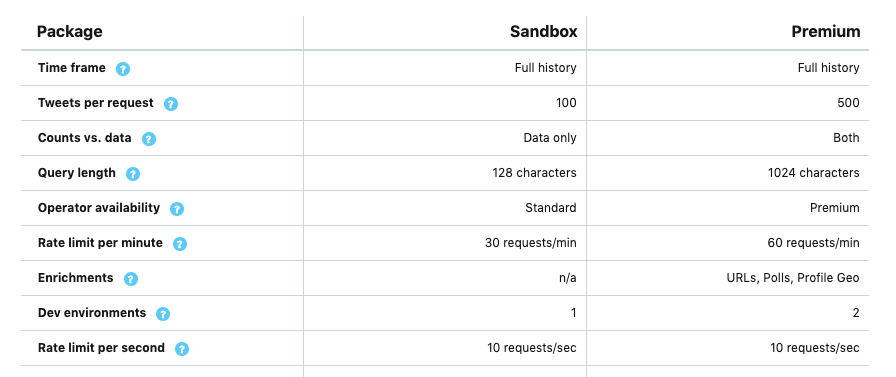
\includegraphics[width=475px]{api_limits} \caption{Twitter Full-Archive Search Limits}\label{fig:unnamed-chunk-29}
\end{figure}
In addition to these limits, there are monthly limits which depend on
the level of access that is selected. We chose a 500/month request limit
for this project. Therefore, with 500 requests per month and 500 tweets
per request, we are capped at 250,000 tweets total. This constraint
determined and influenced many decisions of this study, especially in
regard to the choice of players to include in our sample.

\subsection{Chosen Games and Sample}\label{chosen-games-and-sample}

Initially, when beginning this project, we hoped to use individual plays
of a game as the observational level. We looked to use play-by-play data
that was gathered earlier and match the time of plays to the time of
tweets. Included in this dataset were plays from the first six games of
the 2017 season. However, due to discrepencies in the time variables and
other restraints, this was not possible. Regardless, we are choosing to
continue to focus on those specific games. First, we believe that six
games allows us enough time points while still giving us the ability to
gather enough tweets to accurately measure and model sentiments. More
details on this decision are below. Moreover, in 2017 US President
Donald Trump attacked NFL players who had chosen to kneel in support of
Colin Kaepernick on multiple platforms. He went so far as to say ``get
that son of a bitch off the field,'' referring to any black player that
decided to kneel (Graham, 2017). We predict that the increased racial
tension inflated by the president might be measurable in this study.

As seen from the previous study, some players were barely mentioned on
Twitter, even during the most watched football game of the year.
However, we observe that players from two positions in particular were
mentioned a lot: quarterbacks and receivers. To ensure that we could
gather enough tweets to measure sentiments over a single game, we have
decided to limit our sample to only quarterbacks and receivers as they
seem to be the most popular positions on Twitter.

In order to get closer to making causal connections between sentiment
and race, we needed to ensure that there are an equal number of white
and black quarterbacks and receivers. As we have already decided to
focus in on 2017, we began creating our subset by researching which
teams had starting quarterbacks who were black. The total for 2017 was 8
out of 32 teams. Then, we found that four of these eight teams also had
a top receiver who was white and a top receiver who was black. These
four black quarterbacks and the eight corresponding receivers (one white
and one black from each team) made up the first half of the subset. To
create a balanced design, we chose four white quarterbacks by
determining who was the closest in total yards for the 2017 season for
each black quarterback. After ensuring that these quarterbacks' teams
also had a top receiver who was black and a top receiver who was white,
those 12 additional players were added to the subset. In total, tweets
are gathered for the 24 chosen players.

Had we instead randomly chosen 12 white and 12 black players with 8
being quarterbacks and 16 being receivers, the majority of the
quarterbacks would likely have been white and the majority of the
receivers would likely have been black. The reasoning behind this is
that the majority of quarterbacks in the NFL are white whereas the
majority of receivers are black. Had we not purposefully balanced our
design, the race and positions variables would have been confounded and
including them both in our model would add complexity without adding new
information.

Below is a table of the players, their race, position, corresponding
team.
\begin{table}[!h]

\caption[Total Subset of Study 2]{\label{tab:subset}Total Subset of Study 2}
\centering
\begin{tabular}{l|l|l|l}
\hline
Name & Team & Position & Race\\
\hline
Joe Flacco & Baltimore Ravens & QB & W\\
\hline
Nick Boyle & Baltimore Ravens & R & W\\
\hline
Mike Wallace & Baltimore Ravens & R & B\\
\hline
Cam Newton & Carolina Panthers & QB & B\\
\hline
Devin Funchess & Carolina Panthers & R & B\\
\hline
Christian McCaffrey & Carolina Panthers & R & W\\
\hline
Andy Dalton & Cincinnati Bengals & QB & W\\
\hline
Tyler Kroft & Cincinnati Bengals & R & W\\
\hline
A.J. Green & Cincinnati Bengals & R & B\\
\hline
Dak Prescott & Dallas Cowboys & QB & B\\
\hline
Dez Bryant & Dallas Cowboys & R & B\\
\hline
Jason Witten & Dallas Cowboys & R & W\\
\hline
Alex Smith & Kansas City Chiefs & QB & W\\
\hline
Travis Kelce & Kansas City Chiefs & R & W\\
\hline
Tyreek Hill & Kansas City Chiefs & R & B\\
\hline
Carson Wentz & Philadelphia Eagles & QB & W\\
\hline
Zach Ertz & Philadelphia Eagles & R & W\\
\hline
Alshon Jeffrey & Philadelphia Eagles & R & B\\
\hline
Russell Wilson & Seattle Seahawks & QB & B\\
\hline
Doug Baldwin & Seattle Seahawks & R & B\\
\hline
Jimmy Graham & Seattle Seahawks & R & W\\
\hline
Jameis Winston & Tampa Bay Buccaneers & QB & B\\
\hline
Mike Evans & Tampa Bay Buccaneers & R & B\\
\hline
Adam Humphries & Tampa Bay Buccaneers & R & W\\
\hline
\end{tabular}
\end{table}
Further investigation reveals that Tampa Bay had a bye during week 1 of
the 2017 season and Seattle, Dallas, and Cincinnati had byes during week
6 of the 2017 season. Therefore, if we gather tweets for all 6 games, we
would have missing values. Instead, we decided to choose 5 time points
for each team. For the three teams with a bye during week 6, games 1-5
were chosen and for the other 5 teams, games 2-6 were chosen. In total,
we would gather tweets for 24 players across 5 games. This totals 120
different observations. Since we are limited to 250,000 tweets,
approximately 2083 tweets could be gathered per player per game.

These 24 players are added to a data set shown in Table
\ref{tab:subset}. Also included are variables corresponding to their
Twitter handle, race, position, and starting and ending times for each 5
games. It is important to us that the tweets are gathered during game
play in order to limit extraneous factors that could affect sentiments
toward a player. Given that the average NFL game time in 2016 was just
above 3 hours and 8 minutes Schalter (2017), we are limiting the time
period to 3 hours and 15 minutes after the start of the game.

Race is determined by our own perceptions. To avoid our biases, it would
be ideal to determine race by a personally identified racial/ethnic
code. However, this information is not available.

\subsection{Searchtweets and Gathering Tweets using
Python}\label{searchtweets-and-gathering-tweets-using-python}

In Chapter 3, we use a function from the \texttt{rtweet} package in
\texttt{R}. However, there is no package in \texttt{R} that supports the
full-archive search method. Instead, we used a library in Python called
\texttt{searchtweets} (Pigott, 2018). Like in Chapter 3, we are required
to setup and load authentication, first online and then using the
function \texttt{load\_credentials()}.

\small
\begin{Shaded}
\begin{Highlighting}[]
\NormalTok{premium_search_args }\OperatorTok{=}\NormalTok{ load_credentials(}\StringTok{"~/.twitter_keys.yaml"}\NormalTok{,}
\NormalTok{                                          yaml_key}\OperatorTok{=}\StringTok{"search_tweets_api"}\NormalTok{,}
\NormalTok{                                          env_overwrite}\OperatorTok{=}\VariableTok{False}\NormalTok{)}
\end{Highlighting}
\end{Shaded}
\normalsize

The \texttt{.twitter\_keys.yaml} is a file that contains the same
information loaded into the \texttt{create\_token()} function of the
\texttt{rtweet} package. Once the authentication process is complete,
our data is loaded into the environment using the function
\texttt{read\_csv()} from the \texttt{pandas} library (McKinney \&
others, 2010).

\small
\begin{Shaded}
\begin{Highlighting}[]
\NormalTok{data }\OperatorTok{=}\NormalTok{ pandas.read_csv(}\StringTok{"~PATH/final_subset.csv"}\NormalTok{)}
\end{Highlighting}
\end{Shaded}
\normalsize

Given that we have many variables which need to change each time we run
the function to gather tweets, we created three functions to simplify
the process. The first takes a list of team names and filters the data
for players on those teams.

\small
\begin{Shaded}
\begin{Highlighting}[]
\KeywordTok{def}\NormalTok{ get_data(teams):}
\NormalTok{    data_1 }\OperatorTok{=}\NormalTok{ data[data.Team.isin(teams)]}
    \ControlFlowTok{return}\NormalTok{ data_1}
\end{Highlighting}
\end{Shaded}
\normalsize

The second and third functions are more complex. They are almost exactly
the same except that one searches Twitter for the players' full names
and the other searches for their twitter handles. The arguments of these
functions include a data set as well as start and end time identifiers.
From there, either the full names within the player name column or
twitter handles are made into a list. Then, to grab the start and end
times, the first items from the columns that match the start and end
arguments are selected and saved as objects. Once these objects have
been created, the function gathers tweets using two functions from the
\texttt{searchtweets} library: \texttt{gen\_rule\_payload()} and
\texttt{ResultStream()}. The first takes a query, start time, end time,
and maximum results per request specification. Our function loops
through each name or twitter handle and enters it as the query. Then the
start and end objects are used as the start and end times. The maximum
tweets per request, 500, is kept constant. Added to the query is a
string \texttt{-is:retweet}, which limits the tweets to exclude those
which are retweeted. The rule that is specified using the previous
function is then added for the \texttt{rule\_payload} argument of the
\texttt{ResultStream()} function. This second function also requires the
maximum number of results and pages to search through to be specified,
which we kept constant at 2000 and 4, respectively. The final argument
is our authentication object.

Below is the tweet-gathering loop from one of our functions. The entire
function that searches for players' full names can be found in the data
appendix.

\small
\begin{Shaded}
\begin{Highlighting}[]
\CommentTok{#running loop for tweets}
    
\NormalTok{    all_tweets }\OperatorTok{=}\NormalTok{ []}

    \ControlFlowTok{for}\NormalTok{ handle }\KeywordTok{in}\NormalTok{ newtwitter:}

\NormalTok{        rule }\OperatorTok{=}\NormalTok{ gen_rule_payload(handle }\OperatorTok{+} \StringTok{" -is:retweet"}\NormalTok{,}
\NormalTok{                                from_date }\OperatorTok{=}\NormalTok{ start,}
\NormalTok{                                to_date }\OperatorTok{=}\NormalTok{ end,}
\NormalTok{                                results_per_call }\OperatorTok{=} \DecValTok{500}\NormalTok{)}
            
\NormalTok{        rs }\OperatorTok{=}\NormalTok{ ResultStream(rule_payload}\OperatorTok{=}\NormalTok{rule,}
\NormalTok{                          max_results}\OperatorTok{=}\DecValTok{2000}\NormalTok{,}
\NormalTok{                          max_pages}\OperatorTok{=}\DecValTok{4}\NormalTok{,}
                          \OperatorTok{**}\NormalTok{premium_search_args)}

\NormalTok{        tweets2 }\OperatorTok{=} \BuiltInTok{list}\NormalTok{(rs.stream())}

\NormalTok{        [}\BuiltInTok{print}\NormalTok{(tweet.all_text) }\ControlFlowTok{for}\NormalTok{ tweet }\KeywordTok{in}\NormalTok{ tweets2[}\DecValTok{0}\NormalTok{:}\DecValTok{10}\NormalTok{]]}\OperatorTok{;}
        
\NormalTok{        all_tweets.extend(tweets2)}
        
\NormalTok{        time.sleep(}\DecValTok{10}\NormalTok{)}
\end{Highlighting}
\end{Shaded}
\normalsize

The next part of the function selects certain aspects of the twitter
metadata and adds it to columns in a data frame. The metadata we chose
are the tweets, length, tweet id, date, number of likes, number of
retweets, quoted tweet indicator, quoted or retweet indicator, user
enter text, retweeted tweet indicator, user mentions, profile location,
screen name tweet is replying to, time created string, tweet type, and
full text. This data frame which contains these metadata is returned at
the end of our function.

For each set of teams with the same starting and ending times each week,
these three functions are run. Then, the two data frames containing the
tweets and corresponding metadata are saved as files. Below is an
example.

\small
\begin{Shaded}
\begin{Highlighting}[]
\CommentTok{#specifying teams with the same start and end times for week 1}
\NormalTok{teams }\OperatorTok{=}\NormalTok{ [}\StringTok{"Kansas City Chiefs"}\NormalTok{, }\StringTok{"Tampa Bay Buccaneers"}\NormalTok{, }\StringTok{"Baltimore Ravens"}\NormalTok{,}
\StringTok{"Philadelphia Eagles"}\NormalTok{, }\StringTok{"Carolina Panthers"}\NormalTok{]}
\CommentTok{#filtering for those players}
\NormalTok{data_t1_1 }\OperatorTok{=}\NormalTok{ get_data(teams)}

\CommentTok{#gathering tweets}
\NormalTok{data_t1_1_tweets }\OperatorTok{=}\NormalTok{ get_tweets_name(data_t1_1, start }\OperatorTok{=} \StringTok{'T1_start'}\NormalTok{,}
\NormalTok{                                              end }\OperatorTok{=} \StringTok{'T1_end'}\NormalTok{)}
\NormalTok{data_t1_1_tweetsH }\OperatorTok{=}\NormalTok{ get_tweets_handle(data_t1_1, start }\OperatorTok{=} \StringTok{'T1_start'}\NormalTok{,}
\NormalTok{                                                 end }\OperatorTok{=} \StringTok{'T1_end'}\NormalTok{)}

\CommentTok{#saving tweets/metadata as .csv}
\NormalTok{data_t1_2_tweets.to_csv(}\StringTok{"~PATH/tweets_t1_1.csv"}\NormalTok{, index }\OperatorTok{=} \VariableTok{False}\NormalTok{)}
\NormalTok{data_t1_2_tweetsH.to_csv(}\StringTok{"~PATH/tweets_t1_1_H.csv"}\NormalTok{, index }\OperatorTok{=} \VariableTok{False}\NormalTok{)}
\end{Highlighting}
\end{Shaded}
\normalsize

After gathering tweets for all of the teams for each time point (week of
games), all of the data frames are combined. That larger data frame is
then saved as a file.

\small
\begin{Shaded}
\begin{Highlighting}[]
\CommentTok{#binding tweets from t1 together}
\NormalTok{T1 }\OperatorTok{=}\NormalTok{ pd.concat([data_t1_1_tweets, data_t1_2_tweets, }
\NormalTok{                data_t1_3_tweets, data_t1_4_tweets, }
\NormalTok{                data_t1_1_tweetH, data_t1_2_tweetsH,}
\NormalTok{                data_t1_3_tweetsH, data_t1_4_tweetsH])}

\CommentTok{#saving as .csv}
\NormalTok{T1.to_csv(}\StringTok{"~PATH/tweets_t1_all.csv"}\NormalTok{, index }\OperatorTok{=} \VariableTok{False}\NormalTok{)}
\end{Highlighting}
\end{Shaded}
\normalsize

\subsection{Updating cleaning and sentiment analysis from the Super
Bowl}\label{updating-cleaning-and-sentiment-analysis-from-the-super-bowl}

We then load the data frames containing the tweets and metadata from
each time point into \texttt{R} for cleaning. Luckily, these data have
the same format as the data from the first study. Therefore, many of the
same cleaning techniques are used. However, before these data frames are
all combined, a column containing a time identifying string (ex.
\texttt{t\_1} for the tweets from the first week), is added. Then, these
five data frames are combined to create one data frame that contains all
of the gathered tweets.

\small
\begin{Shaded}
\begin{Highlighting}[]
\CommentTok{#loading in the data}
\ControlFlowTok{for}\NormalTok{ (i }\ControlFlowTok{in} \DecValTok{1}\OperatorTok{:}\KeywordTok{length}\NormalTok{(files)) \{}
  
  \KeywordTok{assign}\NormalTok{(}\KeywordTok{paste}\NormalTok{(}\StringTok{"t"}\NormalTok{, i, }\DataTypeTok{sep =} \StringTok{"_"}\NormalTok{), }\KeywordTok{read.csv}\NormalTok{(}\KeywordTok{paste}\NormalTok{(path, files[i], }
                                                  \DataTypeTok{sep =} \StringTok{""}\NormalTok{)))}
  
\NormalTok{\}}

\CommentTok{#adding time column for each df}
\NormalTok{t_}\DecValTok{1}\NormalTok{ <-}\StringTok{ }\NormalTok{t_}\DecValTok{1} \OperatorTok
\StringTok{  }\KeywordTok{mutate}\NormalTok{(}\DataTypeTok{time =} \StringTok{"t_1"}\NormalTok{)}

\NormalTok{t_}\DecValTok{2}\NormalTok{ <-}\StringTok{ }\NormalTok{t_}\DecValTok{2} \OperatorTok
\StringTok{  }\KeywordTok{mutate}\NormalTok{(}\DataTypeTok{time =} \StringTok{"t_2"}\NormalTok{)}

\NormalTok{t_}\DecValTok{3}\NormalTok{ <-}\StringTok{ }\NormalTok{t_}\DecValTok{3} \OperatorTok
\StringTok{  }\KeywordTok{mutate}\NormalTok{(}\DataTypeTok{time =} \StringTok{"t_3"}\NormalTok{)}

\NormalTok{t_}\DecValTok{4}\NormalTok{ <-}\StringTok{ }\NormalTok{t_}\DecValTok{4} \OperatorTok
\StringTok{  }\KeywordTok{mutate}\NormalTok{(}\DataTypeTok{time =} \StringTok{"t_4"}\NormalTok{)}

\NormalTok{t_}\DecValTok{5}\NormalTok{ <-}\StringTok{ }\NormalTok{t_}\DecValTok{5} \OperatorTok
\StringTok{  }\KeywordTok{mutate}\NormalTok{(}\DataTypeTok{time =} \StringTok{"t_5"}\NormalTok{)}

\CommentTok{#row_binding the three times}
\NormalTok{full <-}\StringTok{ }\KeywordTok{bind_rows}\NormalTok{(t_}\DecValTok{1}\NormalTok{, t_}\DecValTok{2}\NormalTok{, t_}\DecValTok{3}\NormalTok{, t_}\DecValTok{4}\NormalTok{, t_}\DecValTok{5}\NormalTok{)}
\end{Highlighting}
\end{Shaded}
\normalsize

From there, the same cleaning techniques from Chapter 3 are employed.
One final step is to join the tweets with a data frame of the game
outcomes.

\small
\begin{Shaded}
\begin{Highlighting}[]
\NormalTok{tweets_final <-}\StringTok{ }\NormalTok{tweets_final }\OperatorTok
\StringTok{  }\KeywordTok{left_join}\NormalTok{(outcomes, }\DataTypeTok{by =} \KeywordTok{c}\NormalTok{(}\StringTok{"Team"}\NormalTok{, }\StringTok{"time"}\NormalTok{))}
\end{Highlighting}
\end{Shaded}
\normalsize

\subsection{Sentiment Analysis}\label{sentiment-analysis-1}

Again, our functions and techniques from the previous study are employed
with slight variations. From the last study, I found that certain words
commonly used by football fans on Twitter are not included in the
lexicon but are used as positive sentiments. The first step for
sentiment analysis of this study is to add these words as rows to the
end of the bing lexicon data frame.

\small
\begin{Shaded}
\begin{Highlighting}[]
\CommentTok{#creating data frame with additional sentiments}
\NormalTok{extra<-}\KeywordTok{data.frame}\NormalTok{(}\DataTypeTok{word =} \KeywordTok{c}\NormalTok{(}\StringTok{"rings"}\NormalTok{, }\StringTok{"ring"}\NormalTok{, }\StringTok{"history"}\NormalTok{, }\StringTok{"clutch"}\NormalTok{, }
                    \StringTok{"congrats"}\NormalTok{, }\StringTok{"dynasty"}\NormalTok{, }\StringTok{"goat"}\NormalTok{, }\StringTok{"g.o.a.t."}\NormalTok{), }
               \DataTypeTok{sentiment =} \StringTok{"positive"}\NormalTok{)}

\CommentTok{#binding to bing lexicon}
\NormalTok{bing_lex <-}\StringTok{ }\KeywordTok{get_sentiments}\NormalTok{(}\StringTok{"bing"}\NormalTok{)}

\NormalTok{sent_full <-}\StringTok{ }\KeywordTok{bind_rows}\NormalTok{(bing_lex, extra)}
\end{Highlighting}
\end{Shaded}
\normalsize

From there, the same loop run in the previous study could be used if we
wanted the positive and negative word counts for each player across all
five time points. However, for the purpose of our study, we wrote an
altered function that determines the sentiments for each player at each
time point. This was done by adding a time argument that filters the
tweets for that time point. Also, within the function, the other
variables of total sentiment, negative word percentage, positive word
percentage, time, and player name are added to the counts data frame.

\small
\begin{Shaded}
\begin{Highlighting}[]
\NormalTok{sent <-}\StringTok{ }\ControlFlowTok{function}\NormalTok{(t)\{}
  
\CommentTok{#list of names}
\NormalTok{names <-}\StringTok{ }\KeywordTok{as.list}\NormalTok{(subset2}\OperatorTok{$}\NormalTok{name_clean)}

\CommentTok{#list of integers}
\NormalTok{index <-}\StringTok{ }\KeywordTok{as.list}\NormalTok{(}\DecValTok{1}\OperatorTok{:}\KeywordTok{length}\NormalTok{(names))}

\CommentTok{#creating time object to filter df}
\NormalTok{time1 <-}\StringTok{ }\KeywordTok{paste0}\NormalTok{(}\StringTok{"t_"}\NormalTok{, t)}

\NormalTok{add_sentiments <-}\StringTok{ }\ControlFlowTok{function}\NormalTok{(i) \{}
  
  \CommentTok{#filter for each person and the correct time}
\NormalTok{  tweets <-}\StringTok{ }\NormalTok{tweets_final }\OperatorTok
\StringTok{    }\KeywordTok{filter}\NormalTok{(name_clean_final }\OperatorTok{==}\StringTok{ }\NormalTok{names[i],}
\NormalTok{           time }\OperatorTok{==}\StringTok{ }\NormalTok{time1)}
  
  \CommentTok{#one word per row}
\NormalTok{  words <-}\StringTok{ }\NormalTok{tweets }\OperatorTok\StringTok{ }
\StringTok{    }\KeywordTok{select}\NormalTok{(ID, full_text_low) }\OperatorTok\StringTok{ }
\StringTok{    }\KeywordTok{unnest_tokens}\NormalTok{(word,full_text_low)}
  
  \CommentTok{#creating df of stop words  }
\NormalTok{  my_stop_words <-}\StringTok{ }\NormalTok{stop_words }\OperatorTok\StringTok{ }
\StringTok{    }\KeywordTok{select}\NormalTok{(}\OperatorTok{-}\NormalTok{lexicon) }\OperatorTok\StringTok{ }
\StringTok{    }\KeywordTok{bind_rows}\NormalTok{(}\KeywordTok{data.frame}\NormalTok{(}\DataTypeTok{word =} \KeywordTok{c}\NormalTok{(}\StringTok{"https"}\NormalTok{, }\StringTok{"t.co"}\NormalTok{, }\StringTok{"rt"}\NormalTok{, }
                                  \StringTok{"amp"}\NormalTok{,}\StringTok{"4yig9gzh5t"}\NormalTok{,}\StringTok{"fyy2ceydhi"}\NormalTok{,}
                                  \StringTok{"78"}\NormalTok{,}\StringTok{"fakenews"}\NormalTok{)))}

  \CommentTok{#anti-join with stop words to filter those words out}
\NormalTok{  tweet_words <-}\StringTok{ }\NormalTok{words }\OperatorTok\StringTok{ }
\StringTok{    }\KeywordTok{anti_join}\NormalTok{(my_stop_words)}

  \CommentTok{#joining sentiments with non-stop words from tweets}
\NormalTok{  fn_sentiment <-}\StringTok{ }\NormalTok{tweet_words }\OperatorTok\StringTok{ }
\StringTok{    }\KeywordTok{left_join}\NormalTok{(sent_full) }
  
  \CommentTok{#creating df with n of sentiments}
\NormalTok{  df <-}\StringTok{ }\NormalTok{fn_sentiment }\OperatorTok\StringTok{ }
\StringTok{    }\KeywordTok{filter}\NormalTok{(}\OperatorTok{!}\KeywordTok{is.na}\NormalTok{(sentiment)) }\OperatorTok\StringTok{ }
\StringTok{    }\KeywordTok{group_by}\NormalTok{(sentiment) }\OperatorTok\StringTok{ }
\StringTok{    }\KeywordTok{summarise}\NormalTok{(}\DataTypeTok{n=}\KeywordTok{n}\NormalTok{())}

  \CommentTok{#making df of sentiments for each person}
\NormalTok{  df_}\DecValTok{2}\NormalTok{ <-}\StringTok{ }\NormalTok{df }\OperatorTok
\StringTok{  }\KeywordTok{mutate}\NormalTok{(}\DataTypeTok{player =}\NormalTok{ names[i]) }\OperatorTok
\StringTok{  }\KeywordTok{spread}\NormalTok{(}\DataTypeTok{key =}\NormalTok{ sentiment, }\DataTypeTok{value =}\NormalTok{ n)}
  
  \KeywordTok{return}\NormalTok{(df_}\DecValTok{2}\NormalTok{)}
  
\NormalTok{\}}

\CommentTok{#running add sentiment function for each player}
\NormalTok{sentiment_full <-}\StringTok{ }\KeywordTok{map_df}\NormalTok{(index, add_sentiments)}

\CommentTok{#creating percentages}
\NormalTok{sentiment_full <-}\StringTok{ }\NormalTok{sentiment_full }\OperatorTok
\StringTok{  }\KeywordTok{mutate}\NormalTok{(}\DataTypeTok{totalsentiment =}\NormalTok{ negative }\OperatorTok{+}\StringTok{ }\NormalTok{positive,}
         \DataTypeTok{neg_perc =}\NormalTok{ negative}\OperatorTok{/}\NormalTok{totalsentiment }\OperatorTok{*}\StringTok{ }\DecValTok{100}\NormalTok{,}
         \DataTypeTok{pos_perc =}\NormalTok{ positive}\OperatorTok{/}\NormalTok{totalsentiment }\OperatorTok{*}\DecValTok{100}\NormalTok{,}
         \DataTypeTok{time =} \KeywordTok{paste0}\NormalTok{(}\StringTok{"t_"}\NormalTok{, t),}
         \DataTypeTok{player =} \KeywordTok{as.character}\NormalTok{(player))}
  

\KeywordTok{return}\NormalTok{(sentiment_full)}

\NormalTok{\}}
\end{Highlighting}
\end{Shaded}
\normalsize

This function is run 5 times to determine sentiments for each of the
five time points. These are combined to create a data frame with 120
rows (24 players \(\cdot\) 5 time points). Then, it is joined with the
subset dataframe that contains 5 rows per player to include outcome per
time point.

\small
\begin{Shaded}
\begin{Highlighting}[]
\CommentTok{#sentiments for time 1}
\NormalTok{sent_tall_}\DecValTok{1}\NormalTok{ <-}\StringTok{ }\KeywordTok{sent_tall}\NormalTok{(}\DecValTok{1}\NormalTok{)}

\CommentTok{#sentiment for time 2}
\NormalTok{sent_tall_}\DecValTok{2}\NormalTok{ <-}\StringTok{ }\KeywordTok{sent_tall}\NormalTok{(}\DecValTok{2}\NormalTok{)}

\CommentTok{#sentiment for time 3}
\NormalTok{sent_tall_}\DecValTok{3}\NormalTok{ <-}\StringTok{ }\KeywordTok{sent_tall}\NormalTok{(}\DecValTok{3}\NormalTok{)}

\CommentTok{#sentiment for time 4}
\NormalTok{sent_tall_}\DecValTok{4}\NormalTok{ <-}\StringTok{ }\KeywordTok{sent_tall}\NormalTok{(}\DecValTok{4}\NormalTok{)}

\CommentTok{#sentiment for time 5}
\NormalTok{sent_tall_}\DecValTok{5}\NormalTok{ <-}\StringTok{ }\KeywordTok{sent_tall}\NormalTok{(}\DecValTok{5}\NormalTok{)}

\CommentTok{#combining outcome to players}
\NormalTok{outcomes_players <-}\StringTok{ }\NormalTok{subset2 }\OperatorTok
\StringTok{  }\KeywordTok{full_join}\NormalTok{(outcomes, }\DataTypeTok{by =} \StringTok{"Team"}\NormalTok{)}

\CommentTok{#row_binding all of the sentiments together}
\NormalTok{sent_tall_full <-}\StringTok{ }\NormalTok{sent_tall_}\DecValTok{1} \OperatorTok
\StringTok{  }\KeywordTok{bind_rows}\NormalTok{(sent_tall_}\DecValTok{2}\NormalTok{, sent_tall_}\DecValTok{3}\NormalTok{, sent_tall_}\DecValTok{4}\NormalTok{, sent_tall_}\DecValTok{5}\NormalTok{)}

\CommentTok{#joining sentiment tall to outcomes}
\NormalTok{sent_tall_full1 <-}\StringTok{ }\NormalTok{outcomes_players }\OperatorTok
\StringTok{  }\KeywordTok{left_join}\NormalTok{(sent_tall_full, }\DataTypeTok{by =} \KeywordTok{c}\NormalTok{(}\StringTok{"name_clean"}\NormalTok{ =}\StringTok{ "player"}\NormalTok{, }\StringTok{"time"}\NormalTok{))}
\end{Highlighting}
\end{Shaded}
\normalsize

The data frame created here is the final one to be used in our model.
However, one additional variable is added to account for individual
performance during a game. To gather game level data, we use the
\texttt{nflscrapR} package in \texttt{R} (Horowitz, Yurko, \& Ventura,
2019). First, we use the \texttt{scrape\_game\_ids()} function to gather
the game ids for the first 6 weeks of the 2017 season. Then, we filter
for only the teams included in our subset.

\small
\begin{Shaded}
\begin{Highlighting}[]
\CommentTok{#gathering game ids for first 6 weeks in 2017}
\NormalTok{week1_to_}\DecValTok{6}\NormalTok{ <-}\StringTok{ }\KeywordTok{scrape_game_ids}\NormalTok{(}\DecValTok{2017}\NormalTok{, }\DataTypeTok{weeks =} \KeywordTok{c}\NormalTok{(}\DecValTok{1}\NormalTok{, }\DecValTok{2}\NormalTok{, }\DecValTok{3}\NormalTok{, }\DecValTok{4}\NormalTok{, }\DecValTok{5}\NormalTok{, }\DecValTok{6}\NormalTok{))}

\CommentTok{#specifying 8 teams from subset}
\NormalTok{teams <-}\StringTok{ }\KeywordTok{c}\NormalTok{(}\StringTok{"CIN"}\NormalTok{, }\StringTok{"DAL"}\NormalTok{, }\StringTok{"SEA"}\NormalTok{, }\StringTok{"CAR"}\NormalTok{, }\StringTok{"TB"}\NormalTok{, }\StringTok{"PHI"}\NormalTok{, }\StringTok{"KC"}\NormalTok{, }\StringTok{"BAL"}\NormalTok{)}

\CommentTok{#filtering dataset for only those 8 teams}
\NormalTok{week1_to_6_filt <-}\StringTok{ }\NormalTok{week1_to_}\DecValTok{6} \OperatorTok
\StringTok{  }\KeywordTok{filter}\NormalTok{(home_team }\OperatorTok\StringTok{ }\NormalTok{teams }\OperatorTok{|}\StringTok{ }\NormalTok{away_team }\OperatorTok\StringTok{ }\NormalTok{teams)}
\end{Highlighting}
\end{Shaded}
\normalsize

After that, 6 data frames are created that each contain the game ids for
the corresponding week. Weeks 1 and 6 had additional filtering arguments
to filter for the correct teams. From there, a column that includes the
players first initial and last name is added to the subset data frame
(from Table \ref{tab:subset}). For each week, the game ids are added to
a list. A function we wrote, \texttt{get\_stats()}, gathers the stats
for all players from the corresponding game using the
\texttt{player\_game()} function of the \texttt{nflscrapr} package.
Then, we use the \texttt{map\_df} function from the \texttt{purrr}
package to run this function for each game of the week included in the
list (Henry \& Wickham, 2019). Ultimately, this function combines the
data frames from each game. Once the data frame containing all the stats
for the games of that week is constructed, it is filtered for the
players of our subset. The variable of yards per game is creating by
combining the three columns of passing yards, rushing yards, and
receiving yards.

\small
\begin{Shaded}
\begin{Highlighting}[]
\NormalTok{##week 2}
\CommentTok{#game ids added to list}
\NormalTok{week2 <-}\StringTok{ }\KeywordTok{as.list}\NormalTok{(week2}\OperatorTok{$}\NormalTok{game_id)}

\CommentTok{#list of integers}
\NormalTok{index <-}\StringTok{ }\KeywordTok{as.list}\NormalTok{(}\DecValTok{1}\OperatorTok{:}\DecValTok{7}\NormalTok{)}

\CommentTok{#looping through game ids to get stats }
\NormalTok{get_stats <-}\StringTok{ }\ControlFlowTok{function}\NormalTok{(i) \{}
  
\NormalTok{  df <-}\StringTok{ }\KeywordTok{player_game}\NormalTok{(week2[i])}
  
  \KeywordTok{return}\NormalTok{(df)}
  
\NormalTok{\}}

\CommentTok{#stats for all 7 games}
\NormalTok{week2_stats <-}\StringTok{ }\KeywordTok{map_df}\NormalTok{(index, get_stats)}


\CommentTok{#pulling out names}
\NormalTok{names_week2 <-}\StringTok{ }\NormalTok{subset2}\OperatorTok{$}\NormalTok{name_}\DecValTok{2}

\CommentTok{#creating long string of all names}
\NormalTok{all_name2 <-}\StringTok{ }\KeywordTok{paste}\NormalTok{(names_week2, }\DataTypeTok{collapse=}\StringTok{'|'}\NormalTok{)}

\NormalTok{week2_stats <-}\StringTok{ }\NormalTok{week2_stats }\OperatorTok
\StringTok{  }\CommentTok{#filtering for name matches}
\StringTok{  }\KeywordTok{mutate}\NormalTok{(}\DataTypeTok{match =} \KeywordTok{ifelse}\NormalTok{(}\KeywordTok{grepl}\NormalTok{(all_name2, name), }\DecValTok{1}\NormalTok{, }\DecValTok{0}\NormalTok{)) }\OperatorTok
\StringTok{  }\CommentTok{#there is another R.Wilson but we only want the seahawks R.Wilson}
\StringTok{  }\KeywordTok{filter}\NormalTok{(match }\OperatorTok{==}\StringTok{ }\DecValTok{1}\NormalTok{, }\OperatorTok{!}\NormalTok{(name }\OperatorTok{==}\StringTok{ "R.Wilson"} \OperatorTok{&}\StringTok{ }\NormalTok{Team }\OperatorTok{==}\StringTok{ "KC"}\NormalTok{)) }\OperatorTok
\StringTok{  }\KeywordTok{select}\NormalTok{(name, Team,  passyds, rushyds, recyds) }\OperatorTok
\StringTok{  }\CommentTok{#creating full yards and time columns}
\StringTok{  }\KeywordTok{mutate}\NormalTok{(}\DataTypeTok{full_yards =}\NormalTok{ passyds}\OperatorTok{+}\StringTok{ }\NormalTok{rushyds}\OperatorTok{+}\StringTok{ }\NormalTok{recyds,}
         \DataTypeTok{time =} \KeywordTok{ifelse}\NormalTok{(Team }\OperatorTok\StringTok{ }\NormalTok{week_}\DecValTok{1}\NormalTok{, }\StringTok{"t_2"}\NormalTok{, }\StringTok{"t_1"}\NormalTok{)) }\OperatorTok
\StringTok{  }\KeywordTok{select}\NormalTok{(name, Team, full_yards, time)}
\end{Highlighting}
\end{Shaded}
\normalsize

This process is completed for each week. Then, the resulting data frames
are combined and joined on the model data by name and time. One final
adjustment is made to our yards variable in order to standardize yards
for quarterbacks and receivers. As quarterbacks can gain yardage through
multiple receivers but receivers can only gain yardage on their own, the
yards are on two different scales. The common ratio of yards for
quarterbacks to receivers is 3:1, with 300 and 100 yard games for
quarterbacks and receivers, respectively, indicating successful games.
To standardize, the number of total yards for quarterbacks is divided by
3.

\subsection{Modeling}\label{modeling}

As stated earlier, the chosen modeling approach for this project is
multi-level modeling. If a more simple modeling approach was used, we
would not be accounting for the dependence in our data and the estimates
of the coefficients' standard errors would be less accurate. The lowest
level in our data contains the repeated observations for each player.
The variable being measured at that level is the yards per game, which
is a numeric variable greater than zero. The second level in our data is
the player level. The variables being measured at that level are race,
which is a factor variable with factors ``W'' and ``B'' for ``white''
and ``black'', and position, which is a factor variable with factors
``R'' and ``QB'' for ``receiver'' and ``quarterback''. The third level
is the team level. The variable being measured at that level is the game
outcome, which is a factor variable with factors ``W'' and ``L'' for
``win'' and ``loss''. Our goal with the model is to get main effects for
those four variables and an additional main effect for the interaction
term between race and outcome. The results of this model will best help
us answer our research question and test our hypotheses. Below are the
regression equations at each of the three levels then the final equation
combining those three.

Level 1: \(~\)

\(negperc_{tij} = \beta_{0ij} + \beta_{1ij}totalyards_{tij} + \varepsilon_{tij}\)

Level 2: \(~\)

\(\beta_{0ij} = \gamma_{00j} + \gamma_{01j}race_{ij} + \gamma_{02j}position_{ij} + u_{0ij}\)

\(\beta_{1ij} = \gamma_{10j}\)

Level 3: \(~\)

\(\Upsilon_{00j} = \delta_{000} + \delta_{001}outcome_{j} + v_{0j}\)

\(\Upsilon_{01j} = \delta_{010} + \delta_{011}outcome_{j}\)

\(\Upsilon_{02j} = \delta_{020}\)

\(\Upsilon_{10j} = \delta_{100}\)

First, we substitute the equations from level 2 into the equation from
level 1: \(~\)
\begin{align*}
negperc_{tij} = &(\gamma_{00j} + \gamma_{01j}race_{ij} + \gamma_{02j}position_{ij} + u_{0ij}) +\\
&(\gamma_{10j})totalyards_{tij} + \varepsilon_{tij}
\end{align*}
From there, we can substitute in the equations from level 3: \(~\)
\begin{align*}
negperc_{tij} = &\delta_{000} + \delta_{001}outcome_{j} + v_{0j} + \\
&(\delta_{010} + \delta_{011}outcome_{j})race_{ij} + \\
&(\delta_{020})position_{ij} + u_{0ij} +\\
&(\delta_{100})totalyards_{tij} + \varepsilon_{tij}
\end{align*}
In final form, with all of the variables in the correct order, is
written as: \(~\)
\begin{align*}
negperc_{tij} = &\delta_{000} + \delta_{001}outcome_{j} + \delta_{010}race_{ij} \\
&+ \delta_{020}position_{ij} + \delta_{100}totalyards_{tij}\\
&+\delta_{011}outcome_{j}race_{ij} + v_{0j} + u_{0ij} + \varepsilon_{tij}
\end{align*}
The fixed effects of this model include \(\delta_{000}\),
\(\delta_{001}\), \(\delta_{010}\), \(\delta_{020}\), \(\delta_{100}\),
and \(\delta_{020}\). The third level random effects is \(v_{0j}\) which
accounts for the random variance of predicted intercepts (average
percentage of negative words) between teams. The second level random
effect is \(u_{0ij}\), which accounts for random variance of predicted
intercepts for players within teams. Finally, the first level random
effect is \(\varepsilon_{tij}\), which accounts for random variance of
predicted intercepts for players within teams across the five time
points. These random effects are assumed to have means at zero and be
normally distributed:

\(v_{0j} \sim N(0, \tau_{000})\)

\(u_{0ij} \sim N(0, \tau_{001})\)

\(\varepsilon_{tij} \sim N(0, \sigma_{\varepsilon}^2)\)

This model keeps the effect of yards, position, race, and outcome fixed
instead of allowing for variance across players or teams. These
variables are being kept constant because we do not have prior knowledge
that would lead us to believe the effects of these variable are
different across certain players or teams. The three random variance
terms are accounting for the variance in average percentage of negative
words across time points, players, and teams.

There are multiple reasons why we chose to use multilevel regression
modeling instead of regular linear regression modeling. The main reason
we chose this technique is because of the hierarchical nature of our
data. If we did not account for the random variance at each level, we
would be treating each observation as independent when they are not. As
a result, the standard errors will be underestimated and significance
will be overstated. The standard errors for coefficients of higher-level
predictor variables will be most affected. This could lead to more Type
I errors.

A common method to estimate coefficients in multilevel regression is the
maximum likelihood method. This is a general estimation procedure, which
creates estimates of the population parameters that maximize the
probability (maximum likelihood) of observing the data that are actually
observed, given the model. The benefit of this estimation method is that
it is generally robust, and produces estimates that are asymptotically
efficient and consistent. However, in this study, our regression
coefficients are estimated using a slightly altered method, known as
REML (restricted maximum likelihood). During estimation using this
method, only the variance components are a part of the likelihood
function, and the coefficients are estimated in a second estimation
step. This produces parameter estimates with associated standard errors
as well as an overall deviance, which is a function of the likelihood
(Hox, 2010). The reason for using REML instead of the standard ML is due
to our small sample size of 120 observations. The REML method estimates
the random effects after removing the fixed effects of the model. Unlike
other methods, which do not account for the degrees of freedom lost by
estimating fixed effects, REML produces estimates that are less biased
in smaller sample sizes.

To fit the above model in \texttt{R}, the \texttt{lme4} package is used
(Bates, M'achler, Bolker, \& Walker, 2015). The function used is
\texttt{lmer()}, which in our case, takes two arguments: the formula and
the data. Within the formula, we specify our fixed and random effects.
The code used is below.

\small
\begin{Shaded}
\begin{Highlighting}[]
\NormalTok{model <-}\StringTok{ }\KeywordTok{lmer}\NormalTok{(neg_perc }\OperatorTok{~}\StringTok{ }\NormalTok{outcome }\OperatorTok{*}\StringTok{ }\NormalTok{Race }\OperatorTok{+}\StringTok{ }\NormalTok{position }\OperatorTok{+}\StringTok{ }\NormalTok{yards_fixed}
              \OperatorTok{+}\StringTok{ }\NormalTok{(}\DecValTok{1}\OperatorTok{|}\NormalTok{name_}\DecValTok{2}\NormalTok{) }\OperatorTok{+}\StringTok{ }\NormalTok{(}\DecValTok{1}\OperatorTok{|}\NormalTok{Team.x),}
              \DataTypeTok{data =}\NormalTok{ data2)}
\end{Highlighting}
\end{Shaded}
\normalsize

\section{Results}\label{results-1}

\subsection{Summary Statistics}\label{summary-statistics}

The mean percentage of negative words across all time points and players
is 53.6\%. This variable is fairly normally distributed, with a slight
left skew, as shown in Figure \ref{fig:dist}.
\begin{figure}
\centering
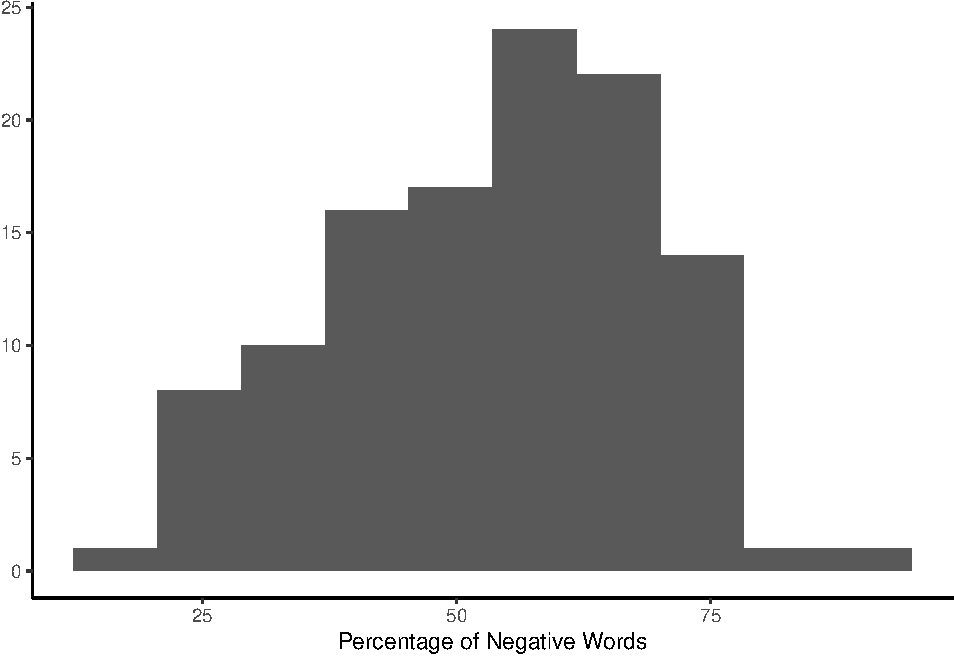
\includegraphics{thesis_files/figure-latex/dist-1.pdf}
\caption{\label{fig:dist}Histogram of Response Variable}
\end{figure}
Next, we hoped to determine the mean percentage of negative words when
breaking down by race and outcome, our two main variables of focus. As
shown in Figure \ref{fig:bargraph}, the median percentage of negative
words for a win is 46.2\% for black players and 46.89\% for white
players. For a loss, the mean percentage of negative words is 65.17\%
for black players and 58.96\%.
\begin{figure}
\centering
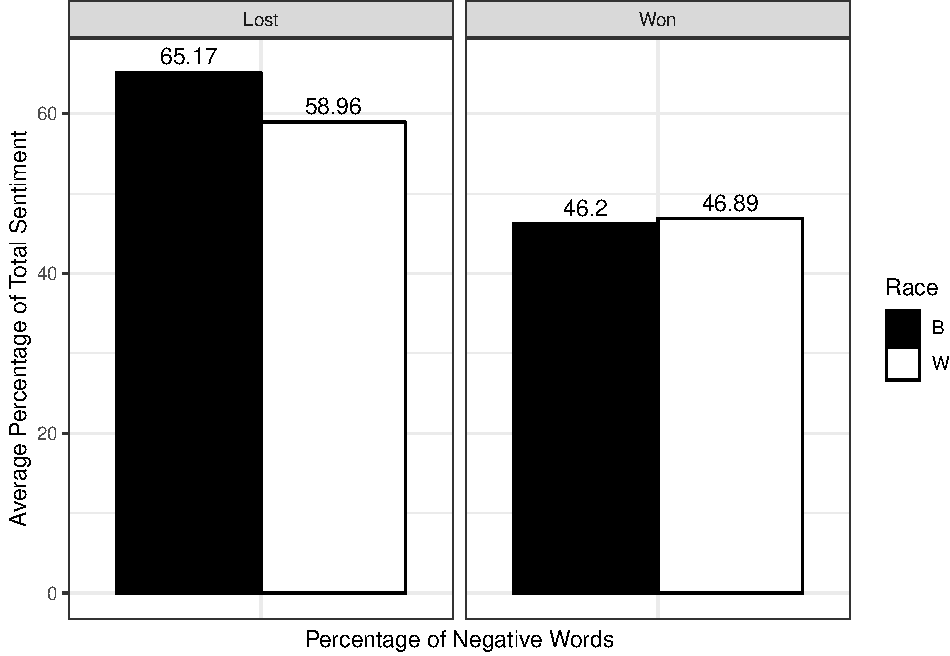
\includegraphics{thesis_files/figure-latex/bargraph-1.pdf}
\caption{\label{fig:bargraph}Mean Percentage of Negative Words across Race
and Outcome}
\end{figure}
\subsection{Missing Data}\label{missing-data}

Tweets in this study are gathered at five different time points for the
24 players. This results in a final \(n\) of 120 observations. However,
6 of these 120 are missing due to a lack of tweets or sentiment words.

\subsection{Multi-level Model}\label{multi-level-model}

Below is Table \ref{tab:tab1} with the results of our model.
\begin{longtable}[]{@{}ccccc@{}}
\caption{\label{tab:tab1} Estimates of \(\delta\) coefficients from our
multilevel regression model}\tabularnewline
\toprule
\begin{minipage}[b]{0.25\columnwidth}\centering\strut
Variable\strut
\end{minipage} & \begin{minipage}[b]{0.15\columnwidth}\centering\strut
Estimation\strut
\end{minipage} & \begin{minipage}[b]{0.15\columnwidth}\centering\strut
St.Error\strut
\end{minipage} & \begin{minipage}[b]{0.15\columnwidth}\centering\strut
p-Value\strut
\end{minipage} & \begin{minipage}[b]{0.17\columnwidth}\centering\strut
95\% CI\strut
\end{minipage}\tabularnewline
\midrule
\endfirsthead
\toprule
\begin{minipage}[b]{0.25\columnwidth}\centering\strut
Variable\strut
\end{minipage} & \begin{minipage}[b]{0.15\columnwidth}\centering\strut
Estimation\strut
\end{minipage} & \begin{minipage}[b]{0.15\columnwidth}\centering\strut
St.Error\strut
\end{minipage} & \begin{minipage}[b]{0.15\columnwidth}\centering\strut
p-Value\strut
\end{minipage} & \begin{minipage}[b]{0.17\columnwidth}\centering\strut
95\% CI\strut
\end{minipage}\tabularnewline
\midrule
\endhead
\begin{minipage}[t]{0.25\columnwidth}\centering\strut
Intercept\strut
\end{minipage} & \begin{minipage}[t]{0.15\columnwidth}\centering\strut
74.21\strut
\end{minipage} & \begin{minipage}[t]{0.15\columnwidth}\centering\strut
4.85\strut
\end{minipage} & \begin{minipage}[t]{0.15\columnwidth}\centering\strut
0.00\strut
\end{minipage} & \begin{minipage}[t]{0.17\columnwidth}\centering\strut
{[}64.92, 83.42{]}\strut
\end{minipage}\tabularnewline
\begin{minipage}[t]{0.25\columnwidth}\centering\strut
OutcomeW\strut
\end{minipage} & \begin{minipage}[t]{0.15\columnwidth}\centering\strut
-19.08\strut
\end{minipage} & \begin{minipage}[t]{0.15\columnwidth}\centering\strut
3.12\strut
\end{minipage} & \begin{minipage}[t]{0.15\columnwidth}\centering\strut
0.00\strut
\end{minipage} & \begin{minipage}[t]{0.17\columnwidth}\centering\strut
{[}-25.19, -13.01{]}\strut
\end{minipage}\tabularnewline
\begin{minipage}[t]{0.25\columnwidth}\centering\strut
RaceW\strut
\end{minipage} & \begin{minipage}[t]{0.15\columnwidth}\centering\strut
-7.22\strut
\end{minipage} & \begin{minipage}[t]{0.15\columnwidth}\centering\strut
3.90\strut
\end{minipage} & \begin{minipage}[t]{0.15\columnwidth}\centering\strut
0.08\strut
\end{minipage} & \begin{minipage}[t]{0.17\columnwidth}\centering\strut
{[}-14.66, 0.21{]}\strut
\end{minipage}\tabularnewline
\begin{minipage}[t]{0.25\columnwidth}\centering\strut
PositionR\strut
\end{minipage} & \begin{minipage}[t]{0.15\columnwidth}\centering\strut
-4.11\strut
\end{minipage} & \begin{minipage}[t]{0.15\columnwidth}\centering\strut
3.24\strut
\end{minipage} & \begin{minipage}[t]{0.15\columnwidth}\centering\strut
0.22\strut
\end{minipage} & \begin{minipage}[t]{0.17\columnwidth}\centering\strut
{[}-10.37, 2.14{]}\strut
\end{minipage}\tabularnewline
\begin{minipage}[t]{0.25\columnwidth}\centering\strut
Fixed Yards\strut
\end{minipage} & \begin{minipage}[t]{0.15\columnwidth}\centering\strut
-0.09\strut
\end{minipage} & \begin{minipage}[t]{0.15\columnwidth}\centering\strut
0.04\strut
\end{minipage} & \begin{minipage}[t]{0.15\columnwidth}\centering\strut
0.02\strut
\end{minipage} & \begin{minipage}[t]{0.17\columnwidth}\centering\strut
{[}-0.16, -0.01{]}\strut
\end{minipage}\tabularnewline
\begin{minipage}[t]{0.25\columnwidth}\centering\strut
OutcomeW:RaceW\strut
\end{minipage} & \begin{minipage}[t]{0.15\columnwidth}\centering\strut
6.72\strut
\end{minipage} & \begin{minipage}[t]{0.15\columnwidth}\centering\strut
4.59\strut
\end{minipage} & \begin{minipage}[t]{0.15\columnwidth}\centering\strut
0.15\strut
\end{minipage} & \begin{minipage}[t]{0.17\columnwidth}\centering\strut
{[}-2.06, 15.82{]}\strut
\end{minipage}\tabularnewline
\bottomrule
\end{longtable}
The resulting formula with the \(\delta\) coefficients included is as
follows:
\begin{align*}
{negperc} = &74.21 - 19.08\widehat{OutcomeW} - 7.22\widehat{RaceW} - 4.11\widehat{PositionR}\\
& - 0.09\widehat{Yards} + 6.74\widehat{OutcomeW*RaceW}
\end{align*}
The intercept (\(\delta_{000}\)) of 74.21 means that the average
percentage of negative words for black players with 0 yards during a
loss is 74.21\%. We are 95\% confident that the true value of the
intercept is between 64.92\% and 83.42\%. The \(\delta_{001}\)
coefficient estimate of -19.08 means that on average, the percentage of
negative words for black players is 19.08 percentage points lower during
a win for the same position and yardage. We are 95\% confident that the
true value of this coefficient is between -25.19\% and -13.01\%. In this
case, The \(\delta_{010}\) coefficient estimate of -7.22 means that on
average, the percentage of negative words during a loss decreases by
7.22\% for white players relative to black players for the same position
and yardage. We are 95\% confident that the true value of this
coefficient is between -14.66\% and 0.21\%. The \(\delta_{020}\)
coefficient estimate of -4.11 means that on average, the percentage of
negative words during a loss for black players decreases by 4.11\% for
receivers, holding yards constant. We are 95\% confident that the true
value of this coefficient is between -10.37\% and 2.14\%. The
\(\delta_{100}\) coefficient estimate of -0.09 means that on average,
for each 1 additional yard gained by a receiver (3 yards for a
quarterback), the percentage of negative words for black players during
a win decreases by 0.09\%, holding position constant. We are 95\%
confident that the true value of this coefficient is between -0.16\% and
-0.01\%. The coefficient estimate of 6.72 for the interaction between
race and outcome means that during a win, the percentage of negative
words for white players increases by 6.72\%, holding position and yards
constant. We are 95\% confident that the true value of this coefficient
is between -2.06\% and 15.82\%.

The coefficient estimates of two of our variables are considered
statistically significant at the p \textless{} 0.05 mark. They are the
outcome and total yards variable. Based on our hypothesis, we expected
race to be a significant predictor of the percentage of negative words.
The p-value for the coefficient estimate of this variable is 0.08 which
technically falls above the significance cutoff. However, the difference
between 0.08 and the significant cutoff of 0.05 is small. We have
purposefully avoided language of statistical significance when
describing the coefficient estimates as the designation of certain
estimates as ``significant'' and ``not significant'' leads some to be
considered ``worthy'' while others are not (Wasserstein, Lazar, \&
others, 2016). Despite our race variable not reaching the arbitrary
significant cutoff, we do not deem the estimate to be unworthy. The
importance of the effect size of this variable cannot be understated, no
matter the p-value. Take the example of Christian McCaffrey, who is
perceived to be white, vs.~Devin Funchess, who is perceived to be black,
both of whom are receivers for the Carolina Panthers. If we compare the
results of our model for these two players during a game that is lost
where they each total 100 yards, the estimates are:

\textbf{For Christian McCaffrey:}
\begin{align*}
{negperc} = &74.21 - 19.08(0) - 7.22(1) - 4.11(1) - 0.09(100) + 6.74(0)
\end{align*}
\begin{align*}
{negperc} = 54%
\end{align*}
\textbf{For Devin Funchess:}
\begin{align*}
{negperc} = &74.21 - 19.08(0) - 7.22(0) - 4.11(1) - 0.09(100) + 6.74(0)
\end{align*}
\begin{align*}
{negperc} = 61%
\end{align*}
Despite an identical performance, these two players have vastly
different amounts of negative sentiment with the only distinguishing
feature between them being their race. To further put these results into
perspective, the difference in negative words percentage between white
and black players during a game that was lost is equal to a difference
of approximately 80 yards for receivers and 240 yards for quarterbacks.
In other words, Devin Funchess would need to gain 80 more yards than
Christian McCaffrey during a game that was lost in order to have the
same observed percentage of negative words.

\subsection{Assumptions}\label{assumptions}

The assumptions for multilevel linear regression are the same as for
simple linear regression. Below, we check the four assumptions of
linearity, normality, homoscedasticity, and independece.

\subsubsection{Linearity}\label{linearity}

The assumption states that there must be a linear relationship between
the explanatory and response variables. This is only applicable for the
relationship between total yards and percentage of negative words as the
other explanatory variables are binary.
\begin{figure}
\centering
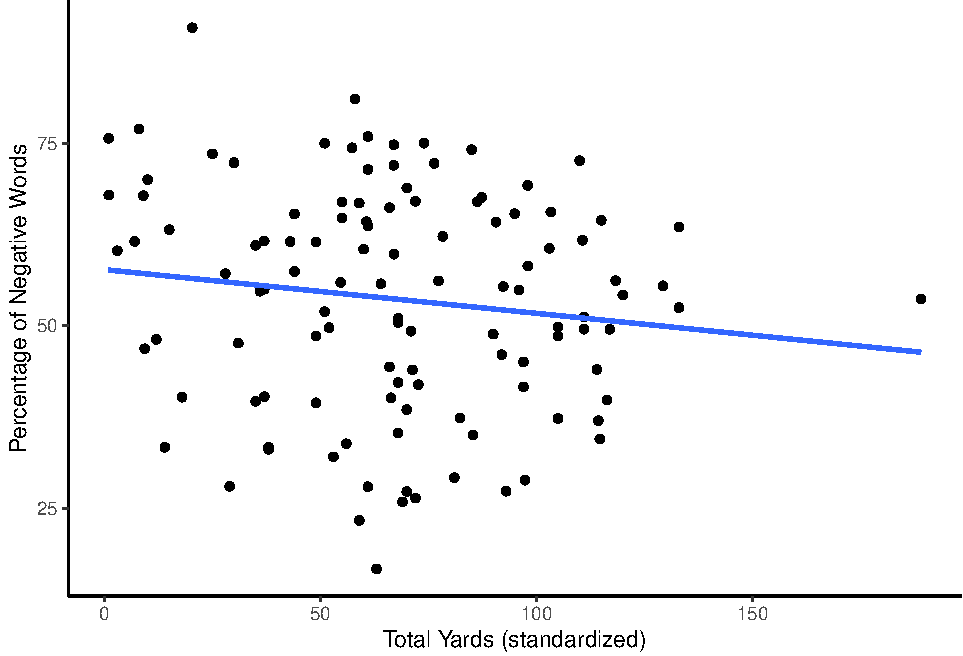
\includegraphics{thesis_files/figure-latex/linearity-1.pdf}
\caption{\label{fig:linearity}Plot of Yards and Percentage of Negative Words
for Linearity Assumption}
\end{figure}
As seen from figure \ref{fig:linearity}, there does appear to be a
negative linear relationship between total yards and percentage of
negative words. Therefore, the linearity assumption is not violated.

\subsubsection{Normality}\label{normality}

The normality assumption states that residuals must be normally
distributed at all levels.
\begin{figure}
\centering
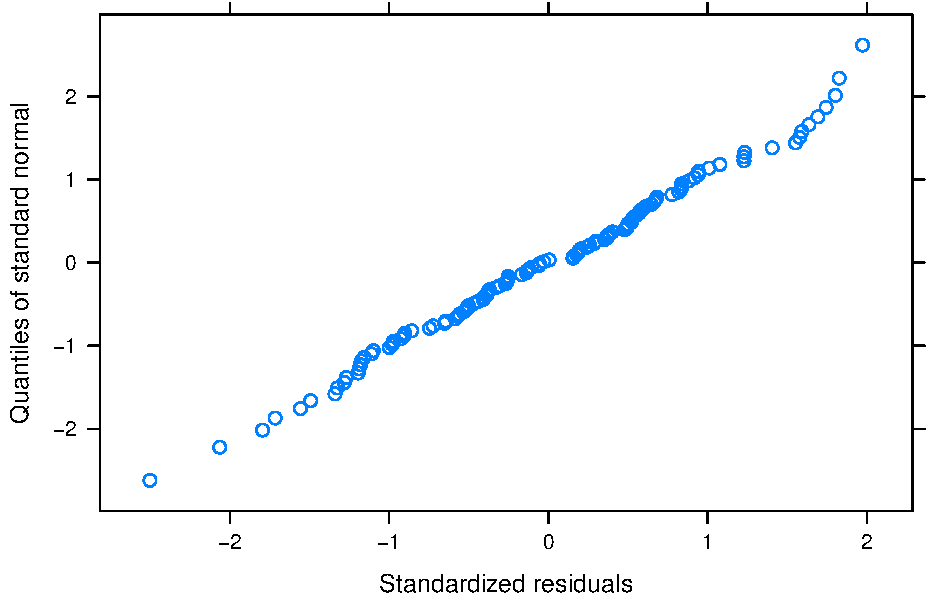
\includegraphics{thesis_files/figure-latex/normal1-1.pdf}
\caption{\label{fig:normal1}Plot of Residual Normality at the First Level in
our Data}
\end{figure}
Figure \ref{fig:normal1} plots the standardized residuals against the
quantiles of standard normal at the first level. It appears that our
residuals are fairly normally distributed.
\begin{figure}
\centering
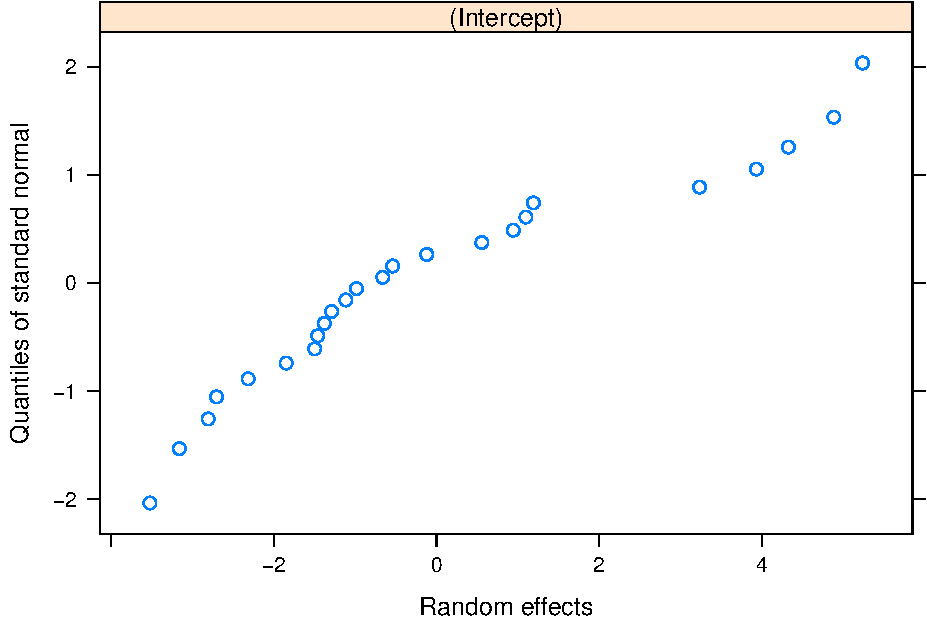
\includegraphics{thesis_files/figure-latex/normal2-1.pdf}
\caption{\label{fig:normal2}Plot of Residual Normality at the Second Level
in our Data}
\end{figure}
Figure \ref{fig:normal2} plots normality of our residuals at the player
level. Like figure \ref{fig:normal1}, it appears that our residuals are
fairly normally distributed at this level.
\begin{figure}
\centering
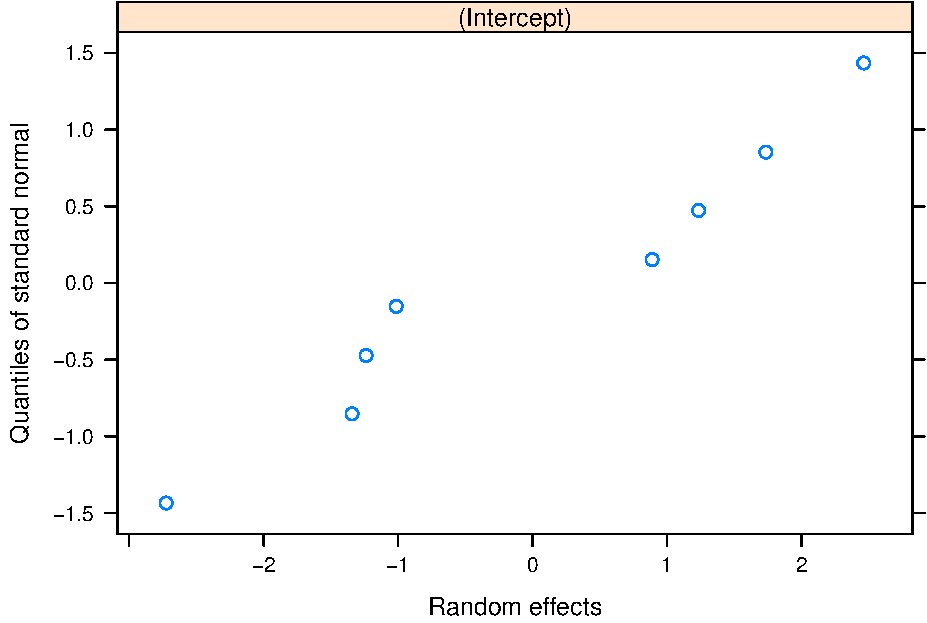
\includegraphics{thesis_files/figure-latex/normal3-1.pdf}
\caption{\label{fig:normal3}Plot of Residual Normality at the Third Level in
our Data}
\end{figure}
The normality of residuals from the team level is displayed in Figure
\ref{fig:normal3}. These residuals appear less normally distributed than
the residuals of the prior levels. However, it is harder to determine
with so few residuals and even so, there does not appear to be enough
evidence to conclude that our residuals are not normally distributed at
this level.

\subsubsection{Homoscedasticity}\label{homoscedasticity}

This assumption states that variances of the residuals must be equal
across groups.
\begin{figure}
\centering
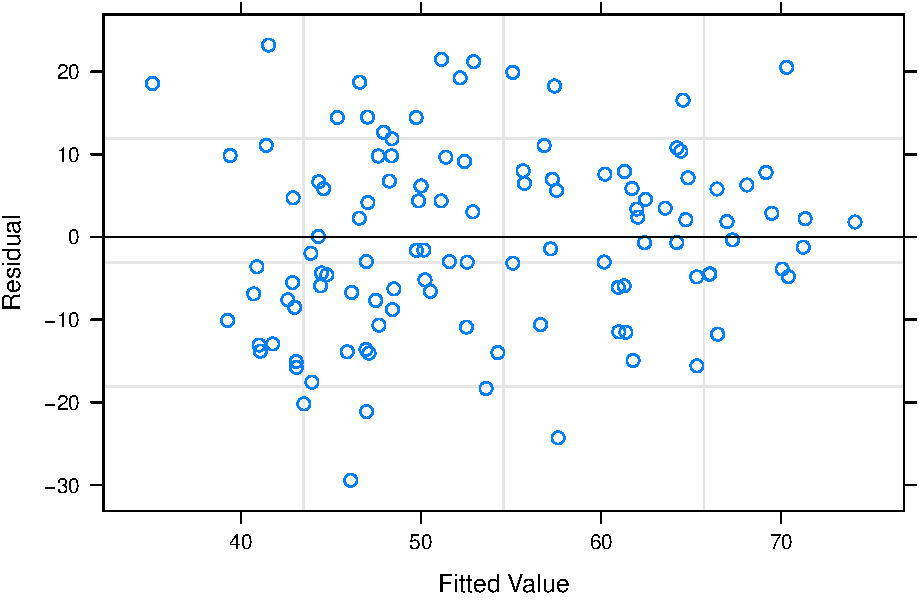
\includegraphics{thesis_files/figure-latex/homosc-1.pdf}
\caption{\label{fig:homosc}Fitted vs.~Residual Plot}
\end{figure}
From Figure \ref{fig:homosc}, there do not appear to be any patterns or
trends in the distribution of the residuals which indicates an equal
variance.

\subsubsection{Independence}\label{independence}

Linear regression assumes that all cases in a sample are independent
from one another. In our case, this would mean that knowing the negative
sentiment of one player at one time point would not help us predict the
negative sentiment of that same player at another time point or another
player entirely. This is not true and is the main reason why multilevel
modeling is necessary. In multilevel modeling, we do additionally assume
that level 1, 2, and 3 residuals are uncorrelated (independent).

\subsection{ICC}\label{icc}

The intraclass correlation (ICC) in multilevel modeling indicates the
proportion of the variance explained by the clustered structure and is
measured by dividing the variance for that level over the total
variance. These calculations are done using the variances from the null
model:
\begin{align*}
negperc_{tij} = \delta_{000} + V_{0j} + &U_{0ij} + \varepsilon_{tij}
\end{align*}
ICC calculation at the team level:

\(~\)

\(ICC_{V_j} = \sigma_{V_j}^2/(\sigma_{V_j}^2+\sigma_{U_{ij}}^2+\sigma_{\epsilon_{tij}}^2)\)

ICC calculation at the player level:

\(~\)

\(ICC_{U_{ij}} = \sigma_{U_{ij}}^2/(\sigma_{V_j}^2+\sigma_{U_{ij}}^2+\sigma_{\epsilon_{tij}}^2)\)

\(~\)

For our model, the ICC is 0.05 for level 3 (team level) and 0.007 for
level 2 (player level). These numbers inform us that we have very little
team variance and even less player variance. So, generally, this means
that there is little evidence that football fans on Twitter feel more or
less negatively about certain teams or certain players. The extremely
small value at the player level may indicate that adding the random
effect for players to our model is not neccesary. However, when running
our 3 level model, we realize that instead of decreasing, the ICC at the
player level increases to 0.12. We expect that when adding predictors,
more of the random variance at the player and team levels would be
explained by the model. While this is the case at the team level, it is
not at the player level.

We expect there to be random variance between players due to some
players being naturally liked more compared to others. Therefore, we
were surpised that our ICC calculated from the null model is so small.
To investigate this small ICC that increases when adding predictors, we
first determined which variable was causing the largest increase in
player level random variance. We found that this variable is game
outcomes. This suggests that the players with naturally higher
percentages of negative tweets are also on losing teams whereas the
players with naturally lower percentages of negative tweets are also on
winning teams. Essentially, by not looking at differences in outcome,
the natural variance between players is being masked.

After coming to this conclusion, we decided that there is sufficient
evidence that we cannot treat our observations as independent. This
confirms that using multilevel regression to account for the random
variances at the three levels is necessary.

\subsection{Sensitivity Analysis}\label{sensitivity-analysis}

Based on a number of factors discussed above, we decided upon the
three-level multilevel model. The next sections investigate the amount
that our standard errors and p-values change depending on the modeling
method.

\subsubsection{Two-level Model}\label{two-level-model}

Had we not further investigated the low ICC at the player level from our
null model, we may have decided to run a two-level multilevel model that
does not account for the random variance at the player level. In this
case, the results are as follows:
\begin{longtable}[]{@{}ccccc@{}}
\caption{\label{tab:tab2} Estimates of \(\delta\) coefficients from a
two-level multilevel regression model}\tabularnewline
\toprule
\begin{minipage}[b]{0.25\columnwidth}\centering\strut
Variable\strut
\end{minipage} & \begin{minipage}[b]{0.15\columnwidth}\centering\strut
Estimation\strut
\end{minipage} & \begin{minipage}[b]{0.15\columnwidth}\centering\strut
St.Error\strut
\end{minipage} & \begin{minipage}[b]{0.15\columnwidth}\centering\strut
p-Value\strut
\end{minipage} & \begin{minipage}[b]{0.17\columnwidth}\centering\strut
95\% CI\strut
\end{minipage}\tabularnewline
\midrule
\endfirsthead
\toprule
\begin{minipage}[b]{0.25\columnwidth}\centering\strut
Variable\strut
\end{minipage} & \begin{minipage}[b]{0.15\columnwidth}\centering\strut
Estimation\strut
\end{minipage} & \begin{minipage}[b]{0.15\columnwidth}\centering\strut
St.Error\strut
\end{minipage} & \begin{minipage}[b]{0.15\columnwidth}\centering\strut
p-Value\strut
\end{minipage} & \begin{minipage}[b]{0.17\columnwidth}\centering\strut
95\% CI\strut
\end{minipage}\tabularnewline
\midrule
\endhead
\begin{minipage}[t]{0.25\columnwidth}\centering\strut
Intercept\strut
\end{minipage} & \begin{minipage}[t]{0.15\columnwidth}\centering\strut
74.21\strut
\end{minipage} & \begin{minipage}[t]{0.15\columnwidth}\centering\strut
4.71\strut
\end{minipage} & \begin{minipage}[t]{0.15\columnwidth}\centering\strut
0.00\strut
\end{minipage} & \begin{minipage}[t]{0.17\columnwidth}\centering\strut
{[}65.13, 83.23{]}\strut
\end{minipage}\tabularnewline
\begin{minipage}[t]{0.25\columnwidth}\centering\strut
OutcomeW\strut
\end{minipage} & \begin{minipage}[t]{0.15\columnwidth}\centering\strut
-19.37\strut
\end{minipage} & \begin{minipage}[t]{0.15\columnwidth}\centering\strut
3.23\strut
\end{minipage} & \begin{minipage}[t]{0.15\columnwidth}\centering\strut
0.00\strut
\end{minipage} & \begin{minipage}[t]{0.17\columnwidth}\centering\strut
{[}-25.57, -13.08{]}\strut
\end{minipage}\tabularnewline
\begin{minipage}[t]{0.25\columnwidth}\centering\strut
RaceW\strut
\end{minipage} & \begin{minipage}[t]{0.15\columnwidth}\centering\strut
-7.35\strut
\end{minipage} & \begin{minipage}[t]{0.15\columnwidth}\centering\strut
3.54\strut
\end{minipage} & \begin{minipage}[t]{0.15\columnwidth}\centering\strut
0.04\strut
\end{minipage} & \begin{minipage}[t]{0.17\columnwidth}\centering\strut
{[}-14.18, -0.50{]}\strut
\end{minipage}\tabularnewline
\begin{minipage}[t]{0.25\columnwidth}\centering\strut
PositionR\strut
\end{minipage} & \begin{minipage}[t]{0.15\columnwidth}\centering\strut
-3.90\strut
\end{minipage} & \begin{minipage}[t]{0.15\columnwidth}\centering\strut
2.66\strut
\end{minipage} & \begin{minipage}[t]{0.15\columnwidth}\centering\strut
0.15\strut
\end{minipage} & \begin{minipage}[t]{0.17\columnwidth}\centering\strut
{[}-9.02, 1.28{]}\strut
\end{minipage}\tabularnewline
\begin{minipage}[t]{0.25\columnwidth}\centering\strut
Fixed Yards\strut
\end{minipage} & \begin{minipage}[t]{0.15\columnwidth}\centering\strut
-0.09\strut
\end{minipage} & \begin{minipage}[t]{0.15\columnwidth}\centering\strut
0.04\strut
\end{minipage} & \begin{minipage}[t]{0.15\columnwidth}\centering\strut
0.02\strut
\end{minipage} & \begin{minipage}[t]{0.17\columnwidth}\centering\strut
{[}-0.16, -0.01{]}\strut
\end{minipage}\tabularnewline
\begin{minipage}[t]{0.25\columnwidth}\centering\strut
OutcomeW:RaceW\strut
\end{minipage} & \begin{minipage}[t]{0.15\columnwidth}\centering\strut
7.42\strut
\end{minipage} & \begin{minipage}[t]{0.15\columnwidth}\centering\strut
4.68\strut
\end{minipage} & \begin{minipage}[t]{0.15\columnwidth}\centering\strut
0.12\strut
\end{minipage} & \begin{minipage}[t]{0.17\columnwidth}\centering\strut
{[}-1.63, 16.46{]}\strut
\end{minipage}\tabularnewline
\bottomrule
\end{longtable}
Compared to the p-values from table \ref{tab:tab1}, those from
\ref{tab:tab2} are all smaller.

\subsubsection{Linear Regression Model}\label{linear-regression-model}

Another method to model this data would be linear regression that is not
heirarchical. The results of this model do not pick up any of the random
variance at the player or team levels of our data.
\begin{longtable}[]{@{}ccccc@{}}
\caption{\label{tab:tab3} Estimates of \(\beta\) coefficients from a basic
linear regression model}\tabularnewline
\toprule
\begin{minipage}[b]{0.25\columnwidth}\centering\strut
Variable\strut
\end{minipage} & \begin{minipage}[b]{0.15\columnwidth}\centering\strut
Estimation\strut
\end{minipage} & \begin{minipage}[b]{0.15\columnwidth}\centering\strut
St.Error\strut
\end{minipage} & \begin{minipage}[b]{0.15\columnwidth}\centering\strut
p-Value\strut
\end{minipage} & \begin{minipage}[b]{0.17\columnwidth}\centering\strut
95\% CI\strut
\end{minipage}\tabularnewline
\midrule
\endfirsthead
\toprule
\begin{minipage}[b]{0.25\columnwidth}\centering\strut
Variable\strut
\end{minipage} & \begin{minipage}[b]{0.15\columnwidth}\centering\strut
Estimation\strut
\end{minipage} & \begin{minipage}[b]{0.15\columnwidth}\centering\strut
St.Error\strut
\end{minipage} & \begin{minipage}[b]{0.15\columnwidth}\centering\strut
p-Value\strut
\end{minipage} & \begin{minipage}[b]{0.17\columnwidth}\centering\strut
95\% CI\strut
\end{minipage}\tabularnewline
\midrule
\endhead
\begin{minipage}[t]{0.25\columnwidth}\centering\strut
Intercept\strut
\end{minipage} & \begin{minipage}[t]{0.15\columnwidth}\centering\strut
73.37\strut
\end{minipage} & \begin{minipage}[t]{0.15\columnwidth}\centering\strut
4.57\strut
\end{minipage} & \begin{minipage}[t]{0.15\columnwidth}\centering\strut
0.00\strut
\end{minipage} & \begin{minipage}[t]{0.17\columnwidth}\centering\strut
{[}64.31, 82.43{]}\strut
\end{minipage}\tabularnewline
\begin{minipage}[t]{0.25\columnwidth}\centering\strut
OutcomeW\strut
\end{minipage} & \begin{minipage}[t]{0.15\columnwidth}\centering\strut
-18.92\strut
\end{minipage} & \begin{minipage}[t]{0.15\columnwidth}\centering\strut
3.33\strut
\end{minipage} & \begin{minipage}[t]{0.15\columnwidth}\centering\strut
0.00\strut
\end{minipage} & \begin{minipage}[t]{0.17\columnwidth}\centering\strut
{[}-25.51, -12.31{]}\strut
\end{minipage}\tabularnewline
\begin{minipage}[t]{0.25\columnwidth}\centering\strut
RaceW\strut
\end{minipage} & \begin{minipage}[t]{0.15\columnwidth}\centering\strut
-7.26\strut
\end{minipage} & \begin{minipage}[t]{0.15\columnwidth}\centering\strut
3.66\strut
\end{minipage} & \begin{minipage}[t]{0.15\columnwidth}\centering\strut
0.05\strut
\end{minipage} & \begin{minipage}[t]{0.17\columnwidth}\centering\strut
{[}-14.51, -0.01{]}\strut
\end{minipage}\tabularnewline
\begin{minipage}[t]{0.25\columnwidth}\centering\strut
PositionR\strut
\end{minipage} & \begin{minipage}[t]{0.15\columnwidth}\centering\strut
-3.67\strut
\end{minipage} & \begin{minipage}[t]{0.15\columnwidth}\centering\strut
2.76\strut
\end{minipage} & \begin{minipage}[t]{0.15\columnwidth}\centering\strut
0.19\strut
\end{minipage} & \begin{minipage}[t]{0.17\columnwidth}\centering\strut
{[}-9.15, 1.81{]}\strut
\end{minipage}\tabularnewline
\begin{minipage}[t]{0.25\columnwidth}\centering\strut
Fixed Yards\strut
\end{minipage} & \begin{minipage}[t]{0.15\columnwidth}\centering\strut
-0.08\strut
\end{minipage} & \begin{minipage}[t]{0.15\columnwidth}\centering\strut
0.04\strut
\end{minipage} & \begin{minipage}[t]{0.15\columnwidth}\centering\strut
0.04\strut
\end{minipage} & \begin{minipage}[t]{0.17\columnwidth}\centering\strut
{[}-0.16, -0.004{]}\strut
\end{minipage}\tabularnewline
\begin{minipage}[t]{0.25\columnwidth}\centering\strut
OutcomeW:RaceW\strut
\end{minipage} & \begin{minipage}[t]{0.15\columnwidth}\centering\strut
7.33\strut
\end{minipage} & \begin{minipage}[t]{0.15\columnwidth}\centering\strut
4.87\strut
\end{minipage} & \begin{minipage}[t]{0.15\columnwidth}\centering\strut
0.13\strut
\end{minipage} & \begin{minipage}[t]{0.17\columnwidth}\centering\strut
{[}-2.33, 16.99{]}\strut
\end{minipage}\tabularnewline
\bottomrule
\end{longtable}
Once again, there are differences between Table \ref{tab:tab3} and Table
\ref{tab:tab1} in terms of coefficients, standard errors, and p-values.
While the results of either of the previous two models may appear more
preferable given society's focus on statistical significance, these
models are commiting Type I errors by under-estimating the standard
errors of the coefficients.

\section{Discussion}\label{discussion}

To begin, our results suggest that there is a strong relationship
between outcome and percentage of negative words. The negative direction
of this coefficient, meaning that a win results in a lower percentage of
negative words, assured us that our data is reliable. If the percentage
of negative words increased during a win, we would be suspicious that
our data is not credible. This direction informs us that during a
positive outcome, the percentage of negative words towards players
decreases. This confirms our first hypothesis. The direction of the
other performance variable, total yards, also suggests that better
performance leads to a lower percentage of negative words, another
indication of reliable data.

The main research question for this project mainly involved differences
between white and black players. To reiterate, our research question is:
Are sentiments on Twitter more negative towards black NFL players after
controlling for game outcome, position, and quality of play? We also
hypothesize that during a game that was lost, sentiments would be more
negative toward black players. The negative direction of the race
coefficient confirms this hypothesis. The coefficient estimate indicates
that during a loss, sentiments are more negative towards black players.
However, our interaction variable suggests that this difference is much
smaller during a game that is won. For a white player during a win, the
percentage of a negative words is only 0.5\% (-7.22\% + 6.72\%) lower
compared to black players.

While our model's coefficient estimate for position is negative, meaning
that receivers receive fewer negative sentiments on average than
quarterbacks, this effect size is not as strong. We did not expect there
to be differences between the two positions but included this variable
in order to control for position while investigating the relationship
between race, outcome, and percentage of negative words.

Our results are consistent with other studies that found that language
for black and white football players is unequal, with black players
receiving more negative sentiments than white players, especially during
a loss. This disparity is evidence of Twitter-using football fan's
racial bias, a phenomenon rarely studied without survey data. Unlike
other research, this study uses data on a much larger scale to quantify
previous findings. As stated in Chapter 1, Hylton \& Lawrence (2016)
argue that further research involving more subtle forms of racism and
racial discrimination in sports is necessary. Through this study, one of
our main goals is to shed light on a subtle form of racism which takes
form through racially disproportionate negative language.

\subsection{Limitations and Future
Directions}\label{limitations-and-future-directions}

These results should be considered in light of their limitations. First,
some players are missing data at certain time points. This means that no
positive or negative words were included in the tweets for those players
at that time point. This lowered our already small sample size which can
have an affect on the validity of our results. The small sample size was
partially due to the Twitter API limits. In order to gather enough
tweets to find positive and negative words, we could not have
realistically added more time points. If we were able to gather more
than 250,000 tweets, we could have added more time points while still
gathering enough tweets for sentiment analyses. This would have
increased our sample size and made our estimates more accurate. By doing
so, important relationships may have been revealed.

Additionally, this study only gathers tweets for 24 players, which is a
small subset of the entire NFL roster of quarterbacks and receivers.
With more players added to the study, our results may be more
generalizable. In the future, it would be beneficial to gain greater
access to Twitter's API search. Unfortunately, this would require a
larger monetary contribution which was not possible in the current
study. Luckily, as seen from Study 1, there are other methods of
accessing the API which are free. With enough planning, tweets could be
gathered using the streaming method during the games of the upcoming
season. This would both increase the subset of players and number of
total tweets.

Another limitation to this study is that the race of the players is
based on our perception and could be unreliable. In the future, having
multiple people offering their perceptions of the players' races could
improve results and reduce biases. In addition to the race variable,
adding more demographic data about the players or extra variables of
individual performance could better disseminate the relationship of
interest from our research question.

Nevertheless, these limitations are offset by strengths. The balanced
nature of this study allowed us to get closer to making causal claims of
racial impacts on the percentage of negative words. Furthermore, though
it would have been favorable to gather more tweets, this study used more
data than many previous studies and therefore offers previously untapped
quantitative insights.

\chapter{Final Remarks}\label{final-remarks}

This project began after witnessing qualitative evidence of negative
language aimed at black players in the NFL. Especially following Colin
Kaepernick kneeling to bring awareness to racial injustices in the
United States, the NFL became a controversial topic. The resulting
fallout of these events, in conjunction with previous research
connecting racism and racial inequality in sports contexts, lead us to
our research question and hypotheses. Given the racially charged climate
within the NFL and football fans during the past few years, we believed
that this racially disproportionate language could be observed on a
larger scale and subsequently modeled.

With the use of multilevel modeling techniques, we are able to account
for the hierarchical nature of our data and produce more accurate
coefficient estimates. The most important result of our main study is
that the black players in our study had higher percentages of negative
words on average, accounting for position, game outcome, and individual
performance. This disparity is even more prominent during a game that
was lost, suggesting that blame may be falling on black players instead
of across all players regardless of race.

We urge researchers to continue to use Twitter and other social media
data to investigate racism and racial inequality within sports contexts.
Data driven insights can be particularly compelling, especially as
research and policy begins to rely even more heavily on big data during
decision-making processes.

\appendix

\chapter{Data Appendix}\label{data-appendix}

\subsection{Python function to gather tweets mentioning
names}\label{python-function-to-gather-tweets-mentioning-names}

\small
\begin{Shaded}
\begin{Highlighting}[]
\KeywordTok{def}\NormalTok{ get_tweets_name(data, start, end):}
    
    \CommentTok{#getting the twitter handles}
\NormalTok{    twitter }\OperatorTok{=}\NormalTok{ data.Name.tolist()}

\NormalTok{    newtwitter }\OperatorTok{=}\NormalTok{ []}

    \ControlFlowTok{for}\NormalTok{ i }\KeywordTok{in} \BuiltInTok{range}\NormalTok{(}\BuiltInTok{len}\NormalTok{(twitter)):}
\NormalTok{        a }\OperatorTok{=}\NormalTok{ twitter[i].replace(}\StringTok{"'"}\NormalTok{, }\StringTok{""}\NormalTok{)}
    
\NormalTok{        newtwitter.append(a)}
    
    \BuiltInTok{print}\NormalTok{(newtwitter)}
    
    
    
    \CommentTok{#getting start date}
    
\NormalTok{    start }\OperatorTok{=}\NormalTok{ data[start]}
    
\NormalTok{    start }\OperatorTok{=}\NormalTok{ start.tolist()}

\NormalTok{    start }\OperatorTok{=}\NormalTok{ start[}\DecValTok{0}\NormalTok{].replace(}\StringTok{"'"}\NormalTok{, }\StringTok{""}\NormalTok{)}
    
    \BuiltInTok{print}\NormalTok{(start)}
    
    
    \CommentTok{#getting end date}
    
\NormalTok{    end }\OperatorTok{=}\NormalTok{ data[end]}
    
\NormalTok{    end }\OperatorTok{=}\NormalTok{ end.tolist()}

\NormalTok{    end }\OperatorTok{=}\NormalTok{ end[}\DecValTok{0}\NormalTok{].replace(}\StringTok{"'"}\NormalTok{, }\StringTok{""}\NormalTok{)}
    
    \BuiltInTok{print}\NormalTok{(end)}
    
    
    
    \CommentTok{#running loop for tweets}
    
\NormalTok{    all_tweets }\OperatorTok{=}\NormalTok{ []}

    \CommentTok{#some_tweets = []}

    \CommentTok{#for i in range(4):}

    \ControlFlowTok{for}\NormalTok{ handle }\KeywordTok{in}\NormalTok{ newtwitter:}

\NormalTok{        rule }\OperatorTok{=}\NormalTok{ gen_rule_payload(handle }\OperatorTok{+} \StringTok{" -is:retweet"}\NormalTok{,}
\NormalTok{                                from_date }\OperatorTok{=}\NormalTok{ start,}
\NormalTok{                                to_date }\OperatorTok{=}\NormalTok{ end,}
\NormalTok{                                results_per_call }\OperatorTok{=} \DecValTok{500}\NormalTok{)}
            
\NormalTok{        rs }\OperatorTok{=}\NormalTok{ ResultStream(rule_payload}\OperatorTok{=}\NormalTok{rule,}
\NormalTok{                          max_results}\OperatorTok{=}\DecValTok{2000}\NormalTok{,}
\NormalTok{                          max_pages}\OperatorTok{=}\DecValTok{4}\NormalTok{,}
                          \OperatorTok{**}\NormalTok{premium_search_args)}

\NormalTok{        tweets2 }\OperatorTok{=} \BuiltInTok{list}\NormalTok{(rs.stream())}

\NormalTok{        [}\BuiltInTok{print}\NormalTok{(tweet.all_text) }\ControlFlowTok{for}\NormalTok{ tweet }\KeywordTok{in}\NormalTok{ tweets2[}\DecValTok{0}\NormalTok{:}\DecValTok{10}\NormalTok{]]}\OperatorTok{;}
        
\NormalTok{        all_tweets.extend(tweets2)}
        
\NormalTok{        time.sleep(}\DecValTok{10}\NormalTok{)}
        
    \CommentTok{#all_tweets.extend(some_tweets)}
        
        
        
    \CommentTok{#creating df    }
    
    
    
    \CommentTok{# We create a pandas dataframe as follows:}
\NormalTok{    data_tweets }\OperatorTok{=}\NormalTok{ pd.DataFrame(data}\OperatorTok{=}\NormalTok{[tweet.text }\ControlFlowTok{for}\NormalTok{ tweet }\KeywordTok{in}\NormalTok{ all_tweets], }
\NormalTok{    columns}\OperatorTok{=}\NormalTok{[}\StringTok{'Tweets'}\NormalTok{])}
    
    \CommentTok{#adding more columns}
\NormalTok{    data_tweets[}\StringTok{'len'}\NormalTok{]  }\OperatorTok{=}\NormalTok{ np.array([}\BuiltInTok{len}\NormalTok{(tweet.text) }
    \ControlFlowTok{for}\NormalTok{ tweet }\KeywordTok{in}\NormalTok{ all_tweets])}
\NormalTok{    data_tweets[}\StringTok{'ID'}\NormalTok{]   }\OperatorTok{=}\NormalTok{ np.array([tweet.}\BuiltInTok{id} 
    \ControlFlowTok{for}\NormalTok{ tweet }\KeywordTok{in}\NormalTok{ all_tweets])}
\NormalTok{    data_tweets[}\StringTok{'Date'}\NormalTok{] }\OperatorTok{=}\NormalTok{ np.array([tweet.created_at_datetime }
    \ControlFlowTok{for}\NormalTok{ tweet }\KeywordTok{in}\NormalTok{ all_tweets])}
\NormalTok{    data_tweets[}\StringTok{'Likes'}\NormalTok{]  }\OperatorTok{=}\NormalTok{ np.array([tweet.favorite_count }
    \ControlFlowTok{for}\NormalTok{ tweet }\KeywordTok{in}\NormalTok{ all_tweets])}
\NormalTok{    data_tweets[}\StringTok{'RTs'}\NormalTok{]    }\OperatorTok{=}\NormalTok{ np.array([tweet.retweet_count }
    \ControlFlowTok{for}\NormalTok{ tweet }\KeywordTok{in}\NormalTok{ all_tweets])}
\NormalTok{    data_tweets[}\StringTok{'Quoted'}\NormalTok{] }\OperatorTok{=}\NormalTok{ np.array([tweet.quoted_tweet }
    \ControlFlowTok{for}\NormalTok{ tweet }\KeywordTok{in}\NormalTok{ all_tweets])}
\NormalTok{    data_tweets[}\StringTok{'Q_or_RT'}\NormalTok{] }\OperatorTok{=}\NormalTok{ np.array([tweet.quote_or_rt_text }
    \ControlFlowTok{for}\NormalTok{ tweet }\KeywordTok{in}\NormalTok{ all_tweets])}
\NormalTok{    data_tweets[}\StringTok{'User_ent_text'}\NormalTok{] }\OperatorTok{=}\NormalTok{ np.array([tweet.user_entered_text }
    \ControlFlowTok{for}\NormalTok{ tweet }\KeywordTok{in}\NormalTok{ all_tweets])}
\NormalTok{    data_tweets[}\StringTok{'retweeted_tweet'}\NormalTok{] }\OperatorTok{=}\NormalTok{ np.array([tweet.retweeted_tweet }
    \ControlFlowTok{for}\NormalTok{ tweet }\KeywordTok{in}\NormalTok{ all_tweets])}
\NormalTok{    data_tweets[}\StringTok{'user_mentions'}\NormalTok{] }\OperatorTok{=}\NormalTok{ np.array([tweet.user_mentions }
    \ControlFlowTok{for}\NormalTok{ tweet }\KeywordTok{in}\NormalTok{ all_tweets])}
\NormalTok{    data_tweets[}\StringTok{'profile_location'}\NormalTok{] }\OperatorTok{=}\NormalTok{ np.array([tweet.profile_location }
    \ControlFlowTok{for}\NormalTok{ tweet }\KeywordTok{in}\NormalTok{ all_tweets])}
\NormalTok{    data_tweets[}\StringTok{'in_reply_to_screen_name'}\NormalTok{] }\OperatorTok{=}\NormalTok{ np.array([}
\NormalTok{    tweet.in_reply_to_screen_name }\ControlFlowTok{for}\NormalTok{ tweet }\KeywordTok{in}\NormalTok{ all_tweets])}
\NormalTok{    data_tweets[}\StringTok{'created_at_string'}\NormalTok{] }\OperatorTok{=}\NormalTok{ np.array([tweet.created_at_string }
    \ControlFlowTok{for}\NormalTok{ tweet }\KeywordTok{in}\NormalTok{ all_tweets])}
\NormalTok{    data_tweets[}\StringTok{'tweet_type'}\NormalTok{] }\OperatorTok{=}\NormalTok{ np.array([tweet.tweet_type }
    \ControlFlowTok{for}\NormalTok{ tweet }\KeywordTok{in}\NormalTok{ all_tweets])}
\NormalTok{    data_tweets[}\StringTok{'retweeted_tweet'}\NormalTok{] }\OperatorTok{=}\NormalTok{ np.array([tweet.retweeted_tweet }
    \ControlFlowTok{for}\NormalTok{ tweet }\KeywordTok{in}\NormalTok{ all_tweets])}
\NormalTok{    data_tweets[}\StringTok{'all_text'}\NormalTok{] }\OperatorTok{=}\NormalTok{ np.array([tweet.all_text }
    \ControlFlowTok{for}\NormalTok{ tweet }\KeywordTok{in}\NormalTok{ all_tweets])}
    
    
    \ControlFlowTok{return}\NormalTok{ data_tweets}
\end{Highlighting}
\end{Shaded}
\normalsize

\backmatter

\chapter*{References}\label{references}
\addcontentsline{toc}{chapter}{References}

\markboth{References}{References}

\noindent

\setlength{\parindent}{-0.20in} \setlength{\leftskip}{0.20in}
\setlength{\parskip}{8pt}

\hypertarget{refs}{}
\hypertarget{ref-angelini2014competing}{}
Angelini, J. R., Billings, A. C., MacArthur, P. J., Bissell, K., \&
Smith, L. R. (2014). Competing separately, medaling equally: Racial
depictions of athletes in NBC's primetime broadcast of the 2012 London
Olympic Games. \emph{Howard Journal of Communications}, \emph{25}(2),
115--133.

\hypertarget{ref-awan2014islamophobia}{}
Awan, I. (2014). Islamophobia and Twitter: A typology of online hate
against Muslims on social media. \emph{Policy \& Internet}, \emph{6}(2),
133--150.

\hypertarget{ref-lme4}{}
Bates, D., M'achler, M., Bolker, B., \& Walker, S. (2015). Fitting
linear mixed-effects models using lme4. \emph{Journal of Statistical
Software}, \emph{67}(1), 1--48.
\url{http://doi.org/10.18637/jss.v067.i01}

\hypertarget{ref-baumer2014r}{}
Baumer, B., Cetinkaya-Rundel, M., Bray, A., Loi, L., \& Horton, N. J.
(2014). R markdown: Integrating a reproducible analysis tool into
introductory statistics. \emph{arXiv Preprint arXiv:1402.1894}.

\hypertarget{ref-burdsey2011joke}{}
Burdsey, D. (2011). That joke isn't funny anymore: Racial
microaggressions, color-blind ideology and the mitigation of racism in
English men's first-class cricket. \emph{Sociology of Sport Journal},
\emph{28}(3), 261--283.

\hypertarget{ref-christopherson2007positive}{}
Christopherson, K. M. (2007). The positive and negative implications of
anonymity in Internet social interactions: ``On the Internet, nobody
knows you're a dog''. \emph{Computers in Human Behavior}, \emph{23}(6),
3038--3056.

\hypertarget{ref-cleland2014racism}{}
Cleland, J. (2014). Racism, football fans, and online message boards:
How social media has added a new dimension to racist discourse in
English football. \emph{Journal of Sport and Social Issues},
\emph{38}(5), 415--431.

\hypertarget{ref-cleland2014fans}{}
Cleland, J., \& Cashmore, E. (2014). Fans, racism and British football
in the twenty-first century: The existence of a 'colour-blind' ideology.
\emph{Journal of Ethnic and Migration Studies}, \emph{40}(4), 638--654.

\hypertarget{ref-streamingapi}{}
\emph{Filtering realtime Tweets}. (2019).
\url{https://developer.twitter.com/en/docs/tweets/filter-realtime/api-reference/post-statuses-filter.html};
Twitter Developer.

\hypertarget{ref-floridi2014open}{}
Floridi, L. (2014). Open data, data protection, and group privacy.
\emph{Philosophy \& Technology}, \emph{27}(1), 1--3.

\hypertarget{ref-floridi2016data}{}
Floridi, L., \& Taddeo, M. (2016). What is data ethics? The Royal
Society.

\hypertarget{ref-gonccalves2013comparing}{}
Gonçalves, P., Araújo, M., Benevenuto, F., \& Cha, M. (2013). Comparing
and combining sentiment analysis methods. In \emph{Proceedings of the
first acm conference on online social networks} (pp. 27--38). ACM.

\hypertarget{ref-graham2017donald}{}
Graham, B. A. (2017). Donald Trump blasts NFL anthem protesters:'Get
that son of a bitch off the field'. \emph{The Guardian}.

\hypertarget{ref-hauser2016colin}{}
Hauser, C. (2016). Why Colin Kaepernick didn't stand for the National
Anthem. \emph{Retrieved on November}, \emph{14}, 2016.

\hypertarget{ref-github}{}
\emph{Hello world}. (2019). \emph{GitHub repository}.
\url{https://guides.github.com/activities/hello-world/}; GitHub.

\hypertarget{ref-purrr}{}
Henry, L., \& Wickham, H. (2019). \emph{Purrr: Functional programming
tools}. Retrieved from \url{https://CRAN.R-project.org/package=purrr}

\hypertarget{ref-nflscrapr}{}
Horowitz, M., Yurko, R., \& Ventura, S. (2019). \emph{NflscrapR:
Compiling the NFL play-by-play API for easy use in R}. Retrieved from
\url{https://github.com/maksimhorowitz/nflscrapR}

\hypertarget{ref-hox2010multilevel}{}
Hox, J. J. (2010). \emph{Multilevel analysis: Techniques and
applications} (pp. 40--41). Routledge; 2 edition.

\hypertarget{ref-hu2004mining}{}
Hu, M., \& Liu, B. (2004). Mining and summarizing customer reviews. In
\emph{Proceedings of the tenth international conference on knowledge
discovery and data mining} (pp. 168--177). ACM.

\hypertarget{ref-hylton2016your}{}
Hylton, K., \& Lawrence, S. (2016). ``For your ears only!'' Donald
Sterling and backstage racism in sport. \emph{Ethnic and Racial
Studies}, \emph{39}(15), 2740--2757.

\hypertarget{ref-intravia2018racial}{}
Intravia, J., Piquero, A. R., \& Piquero, N. L. (2018). The racial
divide surrounding United States of America National Anthem protests in
the National Football League. \emph{Deviant Behavior}, \emph{39}(8),
1058--1068.

\hypertarget{ref-rtweet-package}{}
Kearney, M. W. (2018). \emph{Rtweet: Collecting Twitter data}. Retrieved
from \url{https://cran.r-project.org/package=rtweet}

\hypertarget{ref-keum2018racism}{}
Keum, B. T., \& Miller, M. J. (2018). Racism on the Internet:
Conceptualization and recommendations for research. \emph{Psychology of
Violence}, \emph{8}(6), 782.

\hypertarget{ref-king2004offside}{}
King, C. (2004). \emph{Offside racism: Playing the white man}.
Bloomsbury Academic.

\hypertarget{ref-krishnamurthy2009leakage}{}
Krishnamurthy, B., \& Wills, C. E. (2009). On the leakage of personally
identifiable information via online social networks. \emph{Proceedings
of the 2nd ACM Workshop on Online Social Networks}, 7--12.

\hypertarget{ref-kumar2014twitter}{}
Kumar, S., Morstatter, F., \& Liu, H. (2014). \emph{Twitter data
analytics}. Springer.

\hypertarget{ref-landers2016primer}{}
Landers, R. N., Brusso, R. C., Cavanaugh, K. J., \& Collmus, A. B.
(2016). A primer on theory-driven web scraping: Automatic extraction of
big data from the Internet for use in psychological research.
\emph{Psychological Methods}, \emph{21}(4), 475.

\hypertarget{ref-leung2011presenting}{}
Leung, K. (2011). Presenting post hoc hypotheses as a priori: Ethical
and theoretical issues. \emph{Management and Organization Review},
\emph{7}(3), 471--479.

\hypertarget{ref-luke2004multilevel}{}
Luke, D. A. (2004). \emph{Multilevel modeling} (Vol. 143). Sage.

\hypertarget{ref-mckinney2010data}{}
McKinney, W., \& others. (2010). Data structures for statistical
computing in Python. In \emph{Proceedings of the 9th python in science
conference} (Vol. 445, pp. 51--56). Austin, TX.

\hypertarget{ref-meena2007sentence}{}
Meena, A., \& Prabhakar, T. (2007). Sentence level sentiment analysis in
the presence of conjuncts using linguistic analysis. In \emph{European
conference on information retrieval} (pp. 573--580). Springer.

\hypertarget{ref-mittelstadt2016ethics}{}
Mittelstadt, B. D., \& Floridi, L. (2016). The ethics of big data:
Current and foreseeable issues in biomedical contexts. \emph{Science and
Engineering Ethics}, \emph{22}(2), 303--341.

\hypertarget{ref-Mohammad13}{}
Mohammad, S. M., \& Turney, P. D. (2013). Crowdsourcing a word-emotion
association lexicon, \emph{29}(3), 436--465.

\hypertarget{ref-nasukawa2003sentiment}{}
Nasukawa, T., \& Yi, J. (2003). Sentiment analysis: Capturing
favorability using natural language processing. In \emph{Proceedings of
the 2nd international conference on knowledge capture} (pp. 70--77).
ACM.

\hypertarget{ref-national2018data}{}
National Academies of Sciences, Engineering, Medicine, \& others.
(2018). \emph{Data science for undergraduates: Opportunities and
options}. National Academies Press.

\hypertarget{ref-afinn}{}
Nielsen, F. (2011). \emph{AFINN}. Informatics; Mathematical Modelling,
Technical University of Denmark. Retrieved from
\url{http://www2.imm.dtu.dk/pubdb/p.php?6010}

\hypertarget{ref-searchtweets}{}
Pigott, K., F. (2018). \emph{Searchtweets}. Retrieved from
\url{https://github.com/twitterdev/search-tweets-python}

\hypertarget{ref-basepackage}{}
R Core Team. (2018). \emph{R: A language and environment for statistical
computing}. Vienna, Austria: R Foundation for Statistical Computing.
Retrieved from \url{https://www.R-project.org/}

\hypertarget{ref-rainville1977extent}{}
Rainville, R. E., \& McCormick, E. (1977). Extent of covert racial
prejudice in pro football announcers' speech. \emph{Journalism
Quarterly}, \emph{54}(1), 20--26.

\hypertarget{ref-resnick2016researchers}{}
Resnick, B. (2016). Researchers just released profile data on 70,000
OkCupid users without permission. \emph{Vox. Retreived from:
Https://Www.vox.com/2016/5/12/11666116/70000-Okcupid-Users-Data-Release}.

\hypertarget{ref-facebookbreach}{}
Rosen, G. (2018). \emph{Security update}. Facebook. Retrieved from
\url{https://newsroom.fb.com/news/2018/09/security-update/}

\hypertarget{ref-superbowl2017tweets}{}
Sarah Perez. (2017). \emph{Super Bowl posts on social media are up from
last year, but didn't top 2015's record numbers}. Tech Crunch. Retrieved
from
\url{https://techcrunch.com/2017/02/06/super-bowl-posts-on-social-media-are-up-from-last-year-but-didnt-top-2015s-record-numbers/}

\hypertarget{ref-gametime2016}{}
Schalter, T. (2017). \emph{What makes NFL games take so long?}
FiveThirtyEight. Retrieved from
\url{https://fivethirtyeight.com/features/what-makes-nfl-games-take-so-long/}

\hypertarget{ref-tidytext}{}
Silge, J., \& Robinson, D. (2016). Tidytext: Text mining and analysis
using tidy data principles in R. \emph{JOSS}, \emph{1}(3).
\url{http://doi.org/10.21105/joss.00037}

\hypertarget{ref-textmining}{}
Silge, J., \& Robinson, D. (2018). \emph{Text mining with R: A tidy
approach}.

\hypertarget{ref-solomon2019thesisdown}{}
Solomon, N. (2019). \emph{Thesisdown: An updated R markdown thesis
template using the bookdown package}.

\hypertarget{ref-superbowl2018}{}
Statista. (2019). \emph{TV viewership of the Super Bowl in the United
States from 1990-2019 (in millions)}.
\url{https://www.statista.com/statistics/216526/super-bowl-us-tv-viewership/};
Statista.

\hypertarget{ref-stephens2013geography}{}
Stephens, M. (2013). Geography of hate map. Retrieved from
\url{https://users.humboldt.edu/mstephens/hate/hate_map.html}

\hypertarget{ref-stodden2014scientific}{}
Stodden, V. (2014). What scientific idea is ready for retirement.
\emph{Edge}.

\hypertarget{ref-taylor2016no}{}
Taylor, L. (2016). No place to hide? The ethics and analytics of
tracking mobility using mobile phone data. \emph{Environment and
Planning D: Society and Space}, \emph{34}(2), 319--336.

\hypertarget{ref-wallace2015psychology}{}
Wallace, P. (2015). \emph{The psychology of the Internet}. Cambridge
University Press.

\hypertarget{ref-wasserstein2016asa}{}
Wasserstein, R. L., Lazar, N. A., \& others. (2016). The ASA's statement
on p-values: Context, process, and purpose. \emph{The American
Statistician}, \emph{70}(2), 129--133.

\hypertarget{ref-weller2014twitter}{}
Weller, K., Bruns, A., Burgess, J., Mahrt, M., \& Puschmann, C. (2014).
\emph{Twitter and society} (Vol. 89). Peter Lang.

\hypertarget{ref-stringrpackage}{}
Wickham, H. (2019). \emph{Stringr: Simple, consistent wrappers for
common string operations}. Retrieved from
\url{https://CRAN.R-project.org/package=stringr}

\hypertarget{ref-tidyrpackage}{}
Wickham, H., \& Henry, L. (2018). \emph{Tidyr: Easily tidy data with
'spread()' and 'gather()' functions}. Retrieved from
\url{https://CRAN.R-project.org/package=tidyr}

\hypertarget{ref-williams1999race}{}
Williams, D. R. (1999). Race, socioeconomic status, and health the added
effects of racism and discrimination. \emph{Annals of the New York
Academy of Sciences}, \emph{896}(1), 173--188.

\hypertarget{ref-bookdown}{}
Xie, Y. (2016). \emph{Bookdown: Authoring books and technical documents
with R Markdown}. Boca Raton, Florida: Chapman; Hall/CRC. Retrieved from
\url{https://github.com/rstudio/bookdown}

\hypertarget{ref-zhang2009sentiment}{}
Zhang, C., Zeng, D., Li, J., Wang, F.-Y., \& Zuo, W. (2009). Sentiment
analysis of Chinese documents: From sentence to document level.
\emph{Journal of the American Society for Information Science and
Technology}, \emph{60}(12), 2474--2487.


% Index?

\end{document}
